\documentclass[8pt]{extarticle}
%
%
%
%
%
%
%
%
%
%
%
%
%
%
%
%
%
%
%
%
%
%

% ── Platz: Dichte, Zeilenhöhe, Umbruchreserve ────────────────────────
% Müssen VOR styles/30_layout_spacing stehen.
% Dichte und Zeilenhöhe sind getrennt, weil unterschiedlich riskant:
% Abstände sind Leerraum und vertragen jede Skalierung, Zeilenhöhe
% enthält die Schrift selbst — nur in kleinen Schritten senken und
% danach das PDF auf kollidierende Formelzeilen prüfen.
% \def\ZSFDensityFactor{0.85}     % 1    = Referenz, kleiner = dichter
% \def\ZSFLeadingFactor{0.92}     % 0.95 = Referenz, kleiner = enger
%
% Bereichsfaktoren multiplizieren den globalen Faktor für IHREN Bereich —
% für ZSF, die ungleich verteilt sind (box-lastig vs. textlastig).
% \def\ZSFDensityBoxes{1}         % Innen-/Aussenabstände der Inhaltsboxen
% \def\ZSFDensityText{1}          % Absatzabstand im Fliesstext
% \def\ZSFDensityTables{1}        % Zell- und Zeilenabstand in Tabellen
% \def\ZSFDensityStructure{1}     % Polsterung und Abstände der Titelbalken
%
% Freiraum, der vor einem Titelbalken übrig sein muss, sonst bricht die
% Spalte davor um. Grösser = Balken stehen seltener knapp am Spaltenfuss.
% \def\ZSFBreakReserveFactor{1}   % 1 = Referenz
%
% Der Abstand NACH einem Titelbalken — der ganze Abstand bis zum ersten
% Block darunter, Fliesstext wie Box.
% \def\ZSFBarGapFactor{1}         % 1 = Referenz (3pt), kleiner = enger
%
% Schriftgrösse der Diagramm-Beschriftung — beide Stufen gemeinsam.
% \def\ZSFDiagramLabelScale{0.85} % 1 = Referenz, kleiner = kleinere Labels

\input{styles/00_packages}
\input{styles/10_math}

% ── Formelsatz: Summen- und Limes-Grenzen ────────────────────────────
% side = neben dem Zeichen (spart Höhe), stack = darüber/darunter,
% auto = LaTeX entscheidet nach Kontext.
% \SetZSFsumMode{auto}            % auto | side | stack
% \SetZSFlimMode{auto}            % auto | side | stack

% ============================================================
% 11_math_advanced.tex — OPTIONALES Math-Erweiterungsmodul
% ============================================================
% Opt-in: in preamble.tex einkommentieren für mathe-lastige
% Fächer (LinAlg, Analysis). Baut auf 10_math.tex auf und
% ergänzt nur das Delta — keine Basis-Makros duplizieren.
%
% Voraussetzungen (aus 00_packages.tex):
%   - mathtools, unicode-math   (Operatoren, Symbole)
%   - tikz                      (drawbrace / tikzmark / annote)
% ============================================================

% --- Lineare-Algebra-Operatoren ---
\DeclareMathOperator{\Ker}{Ker}
\DeclareMathOperator{\rang}{rang}
\DeclareMathOperator{\Spur}{Spur}
\DeclareMathOperator{\diag}{diag}
\DeclareMathOperator{\spanop}{span}
\DeclareMathOperator{\eig}{eig}
\DeclareMathOperator{\algVfh}{algVfh}
\DeclareMathOperator{\gVfh}{gVfh}
\DeclareMathOperator{\proj}{proj}
\DeclareMathOperator{\sig}{sig}
\DeclareMathOperator{\Adj}{Adj}

% --- Gotisches Im/Re -> moderne aufrechte Operatoren ---
% AtBeginDocument, weil unicode-math seine Symbole ebenfalls erst dort
% definiert — eine Praeambel-Renewcommand wuerde still ueberschrieben.
\AtBeginDocument{%
  \let\oldIm\Im
  \renewcommand{\Im}{\operatorname{Im}}%
  \let\oldRe\Re
  \renewcommand{\Re}{\operatorname{Re}}%
}

% --- TikZ-Klammern für Matrix-Annotationen ---
\usetikzlibrary{decorations.pathreplacing,calc}
% Das optionale Argument sind KNOTEN-OPTIONEN (z.B. xshift), keine Länge. Der
% Default ist deshalb leer: Ein Mass an dieser Stelle liest pgf als
% Pfeilspezifikation und bricht ab ("Unknown arrow tip kind"). Der vertikale
% Versatz der Klammer hängt ohnehin an den Koordinaten, siehe unten.
\newcommand{\tikzmark}[2][]{\tikz[remember picture, overlay, baseline=-0.5ex]\node[#1](#2){};}
% Die Marker von \tikzmark sitzen auf der GRUNDLINIE des Terms. Ohne Versatz
% liegt die Klammer-Sehne genau dort und läuft als waagrechte Linie mitten
% durch die Formel. Der Versatz muss an den Koordinaten hängen, nicht als
% yshift an der Pfadoption: Knoten aus einem anderen Bild (remember picture)
% werden absolut aufgelöst und ignorieren die Pfad-Transformation.
%
% Richtung und Dekoration gehören zusammen, deshalb setzt jeder Stil beides.
% \ZSF@braceSign trägt das Vorzeichen zur Koordinate — die Optionen werden vor
% den Koordinaten ausgewertet, der Wert steht also rechtzeitig.
\makeatletter
\newcommand{\ZSF@braceSign}{-}
\tikzset{
  brace/.style={decorate, decoration={brace},
                /utils/exec=\renewcommand{\ZSF@braceSign}{}},
  brace mirrored/.style={decorate, decoration={brace,mirror},
                /utils/exec=\renewcommand{\ZSF@braceSign}{-}},
}
\newcounter{brace}
\setcounter{brace}{0}
% \drawbrace[stil]{marke links}{marke rechts}
%   brace           — Klammer ÜBER dem Term (Default)
%   brace mirrored  — Klammer UNTER dem Term
\newcommand{\drawbrace}[3][brace]{%
  \refstepcounter{brace}%
  \tikz[remember picture, overlay]\draw[#1]
    ([yshift=\ZSF@braceSign\ZSFbraceDrop]#2.center)--%
    ([yshift=\ZSF@braceSign\ZSFbraceDrop]#3.center)%
    node[pos=0.5, name=brace-\thebrace]{};%
}
\makeatother
\newcommand{\annote}[3][]{%
  \tikz[remember picture, overlay]\node[#1] at (#2) {#3};%
}

%
%
%
%
%
%
%
%
%
%
\newcommand{\ZSFbraceRoom}{\vspace{\dimexpr\ZSFbraceDrop+\ZSFspaceM\relax}}

% --- Asterisk-Definitionen (mathabx-Namen auf Standard-Symbole) ---
\newcommand{\asterisk}{\ast}
\newcommand{\oasterisk}{\circledast}

%
%
%
%
%
%
%
%
%
%
%
%
%
%
%
%
%
%
%
%
%
%
%
%
\makeatletter
\newcommand{\ZSF@augStretch}{\ZSFtableArrayStretch}
\newcommand{\ZSF@augOpen}{(}   % chktex 9
\newcommand{\ZSF@augClose}{)}  % chktex 9
\pgfkeys{
  /zsf/augmatrix/.is family, /zsf/augmatrix,
  rows/.is choice,
  rows/normal/.code={\renewcommand{\ZSF@augStretch}{\ZSFtableArrayStretch}},
  rows/roomy/.code ={\renewcommand{\ZSF@augStretch}{\ZSFtableArrayStretchRoomy}},
  rows/tight/.code ={\renewcommand{\ZSF@augStretch}{\ZSFtableArrayStretchTight}},
  delims/.is choice,
  delims/paren/.code  ={\renewcommand{\ZSF@augOpen}{(}\renewcommand{\ZSF@augClose}{)}},   % chktex 9
  delims/bracket/.code={\renewcommand{\ZSF@augOpen}{[}\renewcommand{\ZSF@augClose}{]}},   % chktex 9
  delims/none/.code   ={\renewcommand{\ZSF@augOpen}{.}\renewcommand{\ZSF@augClose}{.}},
  ZSF@augDefaults/.style={rows=normal, delims=paren},
}
\NewDocumentEnvironment{ZSFaugmatrix}{O{} m m}
  {\pgfkeys{/zsf/augmatrix, ZSF@augDefaults, #1}%
   \renewcommand{\arraystretch}{\ZSF@augStretch}%
   \left\ZSF@augOpen\begin{array}{@{}*{#2}{c}|*{#3}{c}@{}}}
  {\end{array}\right\ZSF@augClose}
\makeatother
   % opt-in: LinAlg — Ker/rang/Spur/proj/Im/Re,
%
%
%
%
%
%
%
%
%
\ifdefined\ZSFShowcaseMode
  \input{styles/12_plots}
\fi
% ============================================================
% 20_tables.tex — Tabellen-Helfer (semantisches Table-System)
% ============================================================
% Zentrales Design-Prinzip:
%   1. Tabellen fuellen IMMER \linewidth (kein manuelles p{0.16..}).
%   2. Spaltenbreiten werden PROPORTIONAL deklariert (Y{0.18} L{0.54} ...),
%      sodass die Summe der Faktoren = Anzahl X-Spalten ergibt.
%   3. Zebra-Streifen + Header-Highlight sind ins Environment eingebaut;
%      direkte Farb-Primitive sind in Kapiteln per Linter verboten.
%
% Damit ist strukturell ausgeschlossen:
%   - zu kurze Zebra-Streifen (Tabelle schmaler als Box),
%   - überstehende Zeilen (Content sprengt Box-Breite),
%   - Drift zwischen Kapiteln (jede Tabelle nutzt dieselben Wrapper).

% ------------------------------------------------------------
% Spaltentypen (tabularx-X-Varianten)
% ------------------------------------------------------------
% Feste Varianten — jede zaehlt als Faktor 1:
% m{#1}: X-Spalten vertikal mittig (Text + Grafik in einer Zeile).
\renewcommand{\tabularxcolumn}[1]{m{#1}}
\newcolumntype{L}{>{\RaggedRight\arraybackslash}X}   % linksbuendig, umbricht
\newcolumntype{C}{>{\Centering\arraybackslash}X}     % zentriert,  umbricht
\newcolumntype{R}{>{\RaggedLeft\arraybackslash}X}    % rechtsbuendig, umbricht

% Parametrisierte, proportionale Varianten — #1 = relativer Anteil.
%
% WICHTIG (tabularx-Konvention): Die Summe aller Faktoren in EINER
% Tabelle muss = Anzahl X-Spalten sein, damit die Tabelle \linewidth
% voll ausfuellt. L/C/R zählen als Faktor 1.
%
% Beispiele (2 Spalten → Summe 2):
%   Y{0.6}  Y{1.4}            → 30% / 70%
%   Y{1}    Y{1}              → 50% / 50% (== L L)
%   Q{0.8}  Y{1.2}            → 40% / 60%, Spalte 1 rechtsbuendig
% Beispiele (3 Spalten → Summe 3):
%   Y{0.6}  Y{1.5}  Y{0.9}    → 20% / 50% / 30%
%   L       Y{2}    L         → 25% / 50% / 25%
% Beispiele (4 Spalten → Summe 4):
%   Y{1.2}  Y{0.8}  Y{1.2}  Y{0.8}  → 30% / 20% / 30% / 20%
\newcolumntype{Y}[1]{>{\hsize=#1\hsize\RaggedRight\arraybackslash}X} % linksb., proport.
\newcolumntype{Z}[1]{>{\hsize=#1\hsize\Centering\arraybackslash}X}   % zentriert, proport.
\newcolumntype{Q}[1]{>{\hsize=#1\hsize\RaggedLeft\arraybackslash}X}  % rechtsb., proport.

% Zentrierte Formel-Spalte (Math-Mode automatisch, proportional)
\newcolumntype{F}[1]{>{\hsize=#1\hsize\Centering\arraybackslash$}X<{$}}

% ------------------------------------------------------------
% Luft zwischen Zellinhalt und Zeilenkante
% ------------------------------------------------------------
% Der Regler `rows` versprach »mehr Höhe für Zellen mit Brüchen« und konnte
% das nicht halten: \arraystretch skaliert das Zeilenstreben, und ein Streben
% ist ein MINDESTmass. Inhalt, der höher ist als es — ein \dfrac, eine Wurzel,
% ein Bild —, bleibt davon unberührt. Gemessen: an einer Textabelle +22 %
% Höhe, an derselben Tabelle mit \dfrac-Zellen +5 %.
%
% Bündig steht der Inhalt zusätzlich, und zwar unten. Grund ist die
% Ausrichtung der m-Spalte in array.sty (\ar@align@mcell): Ist eine Zelle
% höher als ein Streben, senkt sie den Block um
%   0.5 * (Zellhöhe - Strebenhöhe + \baselineskip)
% und schiebt ihn damit so weit nach unten, dass die Tiefe der Zelle die Tiefe
% der Zeile bestimmt — die ganze verbleibende Luft landet oben. Die Formel ist
% für mehrzeiligen Text gedacht; für eine einzelne hohe Zeile bedeutet sie
% Unterkante bündig. Im Satz sichtbar: Der Nenner eines \dfrac berührte die
% Zeilengrenze, in der letzten Zeile lief er aus der Box.
%
% Kein strebenbasierter Weg behebt das, weil jede Strebe ein Mindestmass ist
% und die Zeilentiefe das Maximum aus Strebe und Zellinhalt. Deshalb meldet
% der Ausrichter die Zelle um \ZSFtableCellPadY höher UND tiefer, ohne sie zu
% verschieben — dieselbe \raisebox-Geste wie bei \ZSFimage, nur eine Ebene
% höher und damit für JEDEN hohen Zellinhalt.
%
% Nur der hohe Zweig wird angefasst. Kurzer Text läuft weiter über die
% Grundlinien-Ausrichtung von array.sty; an ihm ändert sich nichts.
%
% \ar@align@mcell ist ein Hook und keine Interna-Bastelei: array.sty prüft ihn
% selbst mit \ifx\ar@align@mcell\@undefined und setzt ihn in anderen Pfaden
% auf \relax. Die Wache darunter hält den Fall offen, dass eine ältere
% array.sty ihn gar nicht kennt — dann bleibt alles beim Alten.
%
% Bewusst mit TeX-Primitiven und einem EIGENEN Register: \raisebox und die
% \@tempdim*-Register sind hier belegt — colortbl haelt den Farbueberhang der
% Zeile in \@tempdimb/\@tempdimc, und eine Zuweisung darauf wuerde die
% Zeilenflaeche verschieben. Mit \raisebox gemessen: die Zellen kamen leer
% heraus.
\newlength{\ZSFtableCellPadY}
\makeatletter
\newdimen\ZSF@cellShift
\@ifundefined{ar@align@mcell}{}{%
  \def\ar@align@mcell{%
    \ifdim \ht\ar@mcellbox > \ht\strutbox
      \ZSF@cellShift\ht\ar@mcellbox
      \advance\ZSF@cellShift-\ht\@arstrutbox
      \advance\ZSF@cellShift\baselineskip
      \ZSF@cellShift=.5\ZSF@cellShift
      \setbox\ar@mcellbox\hbox{\lower\ZSF@cellShift\box\ar@mcellbox}%
      \ht\ar@mcellbox\dimexpr\ht\ar@mcellbox+\ZSFtableCellPadY\relax
      \dp\ar@mcellbox\dimexpr\dp\ar@mcellbox+\ZSFtableCellPadY\relax
      \box\ar@mcellbox
    \else
      \box\ar@mcellbox
    \fi}%
}
\makeatother

% ------------------------------------------------------------
% Zebra-Streifen (Scannbarkeit)
% ------------------------------------------------------------
\newcommand{\ZSFzebraBG}{\TableZebraColor}
\newcommand{\SetZSFzebraBG}[1]{\renewcommand{\ZSFzebraBG}{#1}}
%
%
%
\newcommand{\ZSFzebraStart}[1]{\rowcolors{#1}{\BoxPlainBackColor}{\ZSFzebraBG}}
\newcommand{\ZSFzebraOff}{\rowcolors{1}{}{}}

% ------------------------------------------------------------
% Header-Highlight
% ------------------------------------------------------------
% Konvention:
%   \ZSFheaderRow   — startet die Header-Zeile und setzt den Zeilen-Hintergrund.
%   \ZSFhead{<Text>} — umschliesst den Inhalt JEDER Header-Zelle (Farbe + bold).
%
% Warum zweigeteilt? In tabularx-X-Spalten propagiert \color, das direkt nach
% \rowcolor am Zeilenanfang gesetzt wird, NICHT zuverlässig über die
% &-Grenzen. Die erste Zelle verliert die Farbe, andere behalten sie — je
% nach Spaltenbreite und Content (siehe SI-Praefix-Bug). Per-Zelle-Wrapper
% via \ZSFhead{...} ist robust und konsistent.
\newcommand{\ZSFheaderRowBG}{\chaptercolor}
\newcommand{\ZSFheaderRowFG}{\chaptercolortext}
\newcommand{\ZSFheaderRow}{\rowcolor{\ZSFheaderRowBG}}
% \ZSFInkOwned steht direkt neben dem \color, das den Kontrast setzt: Die
% Kopfzelle ist eine gesaettigte Flaeche mit eigener Textfarbe, eine
% Inline-Farbe darin waere unlesbar (40_colors_structure -> Ink-Vertrag).
\newcommand{\ZSFhead}[1]{{\color{\ZSFheaderRowFG}\ZSFInkOwned\ZSFfontTableHead #1}}

%
%
%
%
%
%
%
%
%
%
%
%
%
%
%
%
%
%
%
%
%
%
%
%
%
%
%
%
%
%
%
%
%
%
%
%
%
%
%
%
%
%
%
%
\makeatletter
\newcommand{\ZSF@spanBadAlign}[1]{%
  \PackageError{ZSF}{Unbekannte Ausrichtung '#1' in \string\ZSFspan}%
    {Gueltig sind L, C und R -- dieselben Buchstaben wie bei den
     Spaltentypen L/C/R.}%
}
\newcommand{\ZSFspan}[3]{%
  \if L#1\multicolumn{#2}{l}{#3}%
  \else\if R#1\multicolumn{#2}{r}{#3}%
  \else\if C#1\multicolumn{#2}{c}{#3}%
  \else\multicolumn{#2}{c}{\ZSF@spanBadAlign{#1}#3}%
  \fi\fi\fi
}
\makeatother

%
%
%
%
%
%
%
%
%
%
%
%
%
%
%
%
%
%
%
%
%
%
%
%
%
%
%
%
%
%
%
%
%
%
%
%
%
%
\makeatletter
\newif\ifZSF@tblHeader
\newif\ifZSF@tblZebra
\newcommand{\ZSF@tblFont}{\ZSFfontContent}
\newcommand{\ZSF@tblStretch}{\ZSFtableArrayStretch}
\newlength{\ZSF@tblColSep}

%
%
%
%
%
%
%
%
%
%
%
%
%
%
%
%
%
%
%
\newcommand{\ZSF@setRows}[1]{%
  \IfStrEqCase{#1}{%
    {normal}{\renewcommand{\ZSF@tblStretch}{\ZSFtableArrayStretch}%
             \setlength{\ZSFtableCellPadY}{\ZSFDensityTables\ZSFspaceXS}}%
    {roomy} {\renewcommand{\ZSF@tblStretch}{\ZSFtableArrayStretchRoomy}%
             \setlength{\ZSFtableCellPadY}{\ZSFDensityTables\ZSFspaceS}}%
    {tight} {\renewcommand{\ZSF@tblStretch}{\ZSFtableArrayStretchTight}%
             \setlength{\ZSFtableCellPadY}{0pt}}%
  }%
}
\newcommand{\ZSF@setColsep}[1]{%
  \IfStrEqCase{#1}{%
    {normal}{\setlength{\ZSF@tblColSep}{\ZSFtableEdgePad}}%
    {tight} {\setlength{\ZSF@tblColSep}{\ZSFtableEdgePadTight}}%
  }%
}
\newcommand{\ZSF@tblSpec}{}
\newcommand{\ZSF@beginTabularx}[1]{\tabularx{\linewidth}{#1}}
\pgfkeys{
  /zsf/table/.is family, /zsf/table,
  header/.is if=ZSF@tblHeader,
  zebra/.is if=ZSF@tblZebra,
  font/.is choice,
  font/normal/.code={\renewcommand{\ZSF@tblFont}{\ZSFfontContent}},
  font/dense/.code={\renewcommand{\ZSF@tblFont}{\ZSFfontContentDense}},
  % `rows` und `colsep` beantworten ihre Frage EINMAL — die beiden Schlüssel
  % hier reichen sie nur durch (\ZSF@setRows / \ZSF@setColsep, oben). Das
  % valuegrid stellt dieselben zwei Fragen und liest dieselbe Antwort; stünde
  % die Zuordnung an beiden Bausteinen, hiesse `rows=roomy` beim nächsten
  % Eingriff auf einem der beiden etwas anderes.
  rows/.is choice,
  rows/normal/.code={\ZSF@setRows{normal}},
  rows/roomy/.code ={\ZSF@setRows{roomy}},
  rows/tight/.code ={\ZSF@setRows{tight}},
  colsep/.is choice,
  colsep/normal/.code={\ZSF@setColsep{normal}},
  colsep/tight/.code ={\ZSF@setColsep{tight}},
  ZSF@tblDefaults/.style={header=true, zebra=true, font=normal,
                          rows=normal, colsep=normal},
}
\NewDocumentEnvironment{ZSFtable}{O{} m}{%
  \begingroup
  % Zellinhalt: ein \ZSFimage hier bekommt Zellen-, nicht Abbildungshoehe.
  % Explizit und nicht als Default verlassen, damit eine Tabelle IN einer
  % figbox nicht deren Abbildungsbudget erbt (siehe \ZSF@imgBudget, 60_boxes).
  \renewcommand{\ZSF@imgBudget}{\ZSFimageMaxHeight}%
  \pgfkeys{/zsf/table, ZSF@tblDefaults, #1}%
  \setlength{\tabcolsep}{\ZSF@tblColSep}%
  \renewcommand{\arraystretch}{\ZSF@tblStretch}%
  \ZSF@tblFont
  \ifZSF@tblZebra
    \ifZSF@tblHeader\ZSFzebraStart{2}\else\ZSFzebraStart{1}\fi
  \else
    \ZSFzebraOff
  \fi
%
%
%
%
%
%
%
%
%
%
%
%
%
%
%
%
%
%
%
%
%
%
%
%
%
%
%
%
%
%
%
%
%
%
%
  \edef\ZSF@tblSpec{@{\hskip\ZSF@tblColSep}#2@{\hskip\ZSF@tblColSep}}%
  \expandafter\ZSF@beginTabularx\expandafter{\ZSF@tblSpec}%
}{%
  \endtabularx
  \endgroup
}
\makeatother


% ── Tabellen: Zebra-Ton ──────────────────────────────────────────────
% Default folgt der Kapitelfarbe. Ein fester Ton macht Tabellen über alle
% Kapitel hinweg gleich — sinnvoll, wenn die Kapitelfarbe schon woanders trägt.
% \SetZSFzebraBG{\TableZebraColor}

% ============================================================
% 30_layout_spacing.tex — Layout-Grundlagen, Spacing-Skala, Box-Bindungen
% ============================================================

\setlength{\parindent}{0pt}

\widowpenalty=10000
\clubpenalty=10000
\brokenpenalty=4000
\predisplaypenalty=10000

\raggedcolumns
\newcounter{zsfFirstChap}\setcounter{zsfFirstChap}{1}

%
%
%
%
%
%
%
%
%
%
%
%
%
%
%
%
%
%
%
\providecommand{\ZSFDensityFactor}{1}

% ── \ZSFderive: eine Ableitung, die man wiederholen kann ─────────────
% Setzt das Register sofort UND merkt sich die Rechnung. \ZSFChapterDensity
% (unten) laesst die gemerkte Kette in derselben Reihenfolge noch einmal
% laufen und bekommt damit den ganzen Registersatz auf einen neuen Faktor.
%
% Der Grund fuer die Kette statt einer Handvoll Neuberechnungen: Ein Register
% ist eine LAENGE, kein Ausdruck. \ZSFboxPadX hat den Wert, den \ZSFspaceS bei
% seiner Berechnung hatte — die vier Basisregister nachtraeglich zu aendern
% erreicht es nicht mehr. Wer eine neue abgeleitete Groesse anlegt, benutzt
% deshalb \ZSFderive und nicht \setlength; sie faehrt dann von selbst mit.
\makeatletter
\newcommand{\ZSF@spacingChain}{}
\newcommand{\ZSFderive}[2]{%
  \setlength{#1}{#2}%
  \expandafter\gdef\expandafter\ZSF@spacingChain\expandafter{%
    \ZSF@spacingChain\setlength{#1}{#2}}%
}
% Der Dokumentwert, auf den \ZSFChapterDensityReset zurueckstellt. Muss VOR der
% ersten Ableitung gesichert werden, sonst ist er beim Zuruecksetzen schon weg.
\let\ZSF@densityDocument\ZSFDensityFactor

%
%
%
%
%
%
%
%
%
%
%
%
\newcommand{\ZSFChapterDensity}[1]{\def\ZSFDensityFactor{#1}\ZSF@spacingChain
  \ZSFApplyDisplaySkips}
\newcommand{\ZSFChapterDensityReset}{%
  \let\ZSFDensityFactor\ZSF@densityDocument \ZSF@spacingChain
  \ZSFApplyDisplaySkips}
\makeatother

% ── Display-Skips: die EINE Stelle, und sie muss wiederholbar sein ───
% Die engen Abstände um Formeln sind eine ZSF-Entscheidung. LaTeX legt sie
% aber in den Groessenbefehlen ab: \normalsize und \footnotesize setzen alle
% vier Skips auf die KLASSENWERTE zurueck. Jeder Schriftwechsel im Inhalt
% loescht damit die Entscheidung — lautlos, denn Formeln sehen auch mit den
% Klassenwerten korrekt aus, nur luftiger.
%
% Deshalb ist die Politik ein benanntes Makro und kein einmaliges \setlength:
% Wer die Groesse wechselt, ruft sie danach erneut auf. Genutzt von
% \ZSFfontContent/\ZSFfontContentDense (der `font`-Regler), vom
% \AtBeginDocument in 70_document_settings und von \ZSFChapterDensity oben.
% \jot und \arraycolsep laufen hier mit, obwohl kein Groessenbefehl sie
% zuruecksetzt: Sie gehoeren zur selben Frage — »wie viel Luft hat eine
% Formel« — und eine zweite Anwendungsstelle waere eine zweite Auslegung.
\newcommand{\ZSFApplyDisplaySkips}{%
  \setlength{\abovedisplayskip}{\ZSFspaceXS}%
  \setlength{\belowdisplayskip}{\ZSFspaceXS}%
  \setlength{\abovedisplayshortskip}{\ZSFspaceXS}%
  \setlength{\belowdisplayshortskip}{\ZSFspaceXS}%
  \setlength{\mathsurround}{\ZSFspaceXS}%
  \setlength{\jot}{\ZSFmathRowSep}%
  \setlength{\arraycolsep}{\ZSFmathColSep}%
}

\newlength{\ZSFspaceXS}\ZSFderive{\ZSFspaceXS}{\ZSFDensityFactor\dimexpr 1pt\relax}
\newlength{\ZSFspaceS} \ZSFderive{\ZSFspaceS}{\ZSFDensityFactor\dimexpr 4pt\relax}
\newlength{\ZSFspaceM} \ZSFderive{\ZSFspaceM}{\ZSFDensityFactor\dimexpr 7pt\relax}
\newlength{\ZSFspaceL} \ZSFderive{\ZSFspaceL}{\ZSFDensityFactor\dimexpr 10pt\relax}

%
%
%
%
%
%
%
%
%
%
%
%
%
%
%
%
%
%
%
\providecommand{\ZSFDensityBoxes}{1}
\providecommand{\ZSFDensityText}{1}
\providecommand{\ZSFDensityTables}{1}
\providecommand{\ZSFDensityStructure}{1}

% Outer (Text-Box-Bindung) und Sep (Trennlinien) — beide folgen der Dichte.
% Outer ist bewusst als \ZSFspaceM abgeleitet statt erneut ausgeschrieben:
% es IST der Standard-Aussenabstand, kein eigener Wert.
\newlength{\ZSFspaceOuter}\ZSFderive{\ZSFspaceOuter}{\ZSFspaceM}
\newlength{\ZSFspaceSep}  \ZSFderive{\ZSFspaceSep}{\ZSFDensityBoxes\dimexpr
  \ZSFDensityFactor\dimexpr 3pt\relax\relax}

% Absatzabstand im Fliesstext — der grösste einzelne vertikale Posten einer
% ZSF und deshalb der wichtigste Teil der Dichte-Stellschraube. Muss nach den
% Basisregistern stehen, damit \ZSFDensityFactor bereits bekannt ist.
% Der Bereichsfaktor greift über das Zwischenregister: Ein Faktor vor einem
% Skip-Register skaliert Soll-, Streck- und Schrumpfanteil gemeinsam; zwei
% Faktoren direkt hintereinander kann TeX dagegen nicht lesen.
\newlength{\ZSFparskipBase}
\ZSFderive{\ZSFparskipBase}{\ZSFDensityFactor\dimexpr 3.5pt\relax
                    plus \ZSFDensityFactor\dimexpr 1pt\relax
                   minus \ZSFDensityFactor\dimexpr 0.5pt\relax}
\ZSFderive{\parskip}{\ZSFDensityText\ZSFparskipBase}

% ── Zeilenhöhe: die zweite globale Stellschraube ─────────────────────
% Bewusst NICHT an \ZSFDensityFactor gekoppelt. Abstände sind Leerraum und
% vertragen jede Skalierung; Zeilenhöhe enthält die Schrift selbst — sie mit
% demselben Faktor zu stauchen, lässt Formeln und Akzente kollidieren.
% Wer zusätzlich zur Dichte enger setzen will, dreht hier separat:
%   \def\ZSFLeadingFactor{0.92}   % in preamble.tex, vor diesem \input
\providecommand{\ZSFLeadingFactor}{0.95}
\linespread{\ZSFLeadingFactor}

% ------------------------------------------------------------
% Spalten-Layout
% ------------------------------------------------------------
% \columnsep folgt der Dichte bewusst NICHT: Beim Verdichten sollen die
% Zeilen enger stehen, nicht die Spalten zusammenrücken — ein schmalerer
% Steg macht die ZSF schlechter lesbar, obwohl er kaum Platz spart.
\newlength{\ZSFcolumnSep}\setlength{\ZSFcolumnSep}{10pt}
\setlength{\columnsep}{\ZSFcolumnSep}
\setlength{\multicolsep}{\ZSFspaceS}
\setlength{\emergencystretch}{2em}

% ------------------------------------------------------------
% Schwellwerte und Titelbalken-Hilfsgrössen
% ------------------------------------------------------------
% Mindesthöhe, die vor einem Titelbalken frei sein muss — sonst bricht die
% Spalte davor um. Die Reserve muss den Balken UND den Anfang der folgenden
% Box tragen, sonst bleibt der Balken allein am Spaltenende stehen.
% Deshalb staffeln sich die Werte nach der Grösse der eröffneten Einheit:
% Kapitel > Abschnitt > Unterabschnitt.
% Die drei Werte sind EINE Staffelung, kein Trio unabhängiger Zahlen. Wer die
% ZSF früher oder später umbrechen lassen will, dreht deshalb den Faktor und
% nicht die drei Register einzeln — nur so bleibt ihr Verhältnis gewahrt.
% Grösser = die Spalte bricht eher vorzeitig um und lässt
% Balken seltener knapp am Fuss stehen; kleiner = dichter gefüllte Spalten.
\providecommand{\ZSFBreakReserveFactor}{1}
\newlength{\ZSFbreakThresholdChapter}
  \setlength{\ZSFbreakThresholdChapter}{\ZSFBreakReserveFactor\dimexpr 10\baselineskip\relax}
\newlength{\ZSFbreakThreshold}
  \setlength{\ZSFbreakThreshold}{\ZSFBreakReserveFactor\dimexpr 7\baselineskip\relax}
\newlength{\ZSFbreakThresholdSubsubsection}
  \setlength{\ZSFbreakThresholdSubsubsection}{\ZSFBreakReserveFactor\dimexpr 5\baselineskip\relax}
\newlength{\ZSFtitleBarHeight}\setlength{\ZSFtitleBarHeight}{9.2pt}
\newlength{\ZSFsubsectionBarBeforeSkip}\ZSFderive{\ZSFsubsectionBarBeforeSkip}{\ZSFDensityStructure\ZSFspaceL}
\newlength{\ZSFsubsubsectionBarBeforeSkip}\ZSFderive{\ZSFsubsubsectionBarBeforeSkip}{\ZSFDensityStructure\ZSFspaceS}
\newlength{\ZSFsubsectionAfterChapterGap}\ZSFderive{\ZSFsubsectionAfterChapterGap}{\ZSFDensityStructure\ZSFspaceXS}

% ── Der Abstand NACH einem Titelbalken ───────────────────────────────
% EIN Register für alle vier Balken, und es ist der GANZE Abstand von der
% Unterkante des Balkens bis zur Oberkante des folgenden Blocks — Fliesstext
% wie Box. Der Weg dorthin ist \ZSFInterlude (unten), aufgerufen im
% after-Hook \ZSFTitleBarAfter (60_boxes).
%
% Vorher war dieser Abstand herrenlos, und zwar nach demselben Muster wie
% \ZSFBoxBeforeSkip (styles/README → »Abstand hat genau einen Schreiber«):
% Zwei Register (\ZSFchapterBarAfterSkip 2pt, \ZSFsubsectionAfterGap 1pt)
% setzten je EINEN Posten von dreien. Dazu kamen \parskip (3.5pt, weil der
% Text nach dem Balken ein neuer Absatz ist) und die Zeilenschaltung
% (\baselineskip − Höhe der ersten Zeile). Gemessen am Satz: Balken → Box
% 1pt, Balken → Fliesstext 6.8pt, Kapitelbalken → Fliesstext 9.5pt. Drei
% Abstände an derselben Stelle des Systems, keiner davon gewählt.
%
% Der Wert (3pt) liegt zwischen den beiden Zuständen von vorher: enger als der
% Fliesstext-Fall (6.8/9.5pt, den niemand gewählt hatte), etwas luftiger als
% der Box-Fall (1pt, der nur deshalb so knapp war, weil dort kein \parskip
% dazukam). Am Satz geprüft, nicht gerechnet: 2pt drückt den ersten Satz an
% den Balken, 4pt bringt die alte Lücke zurück.
%
% Die Staffelung Kapitel > Abschnitt ist bewusst aufgegeben: Die Ebene wird
% über Balkenhöhe, Farbe und den Abstand DAVOR unterschieden
% (\ZSFsubsectionBarBeforeSkip), nicht über einen Punkt danach.
\providecommand{\ZSFBarGapFactor}{1}
\newlength{\ZSFbarAfterGap}\ZSFderive{\ZSFbarAfterGap}{\ZSFBarGapFactor\dimexpr
  \ZSFDensityStructure\dimexpr\ZSFDensityFactor\dimexpr 3pt\relax\relax\relax}
% Der sichtbare Aussenradius ist Form, nicht Leerraum: Auch bei dichterem Satz
% bleiben die Kanten bewusst gleich weich. Der Innenradius wird aus der
% jeweiligen Rahmenbreite abgeleitet, damit die Kontur in der Kurve nicht
% dicker wird als auf den geraden Kanten.
\newlength{\ZSFboxArc}\setlength{\ZSFboxArc}{3pt}
\newlength{\ZSFboxRuleWidth}\setlength{\ZSFboxRuleWidth}{0.5pt}
\newlength{\ZSFboxInnerArc}\ZSFderive{\ZSFboxInnerArc}{\dimexpr
  \ZSFboxArc-\ZSFboxRuleWidth\relax}
\newlength{\ZSFgoalConditionRuleWidth}\setlength{\ZSFgoalConditionRuleWidth}{1.5pt}
\newlength{\ZSFgoalConditionBorderlineWidth}\setlength{\ZSFgoalConditionBorderlineWidth}{0.2pt}
\newlength{\ZSFgoalConditionInnerArc}\ZSFderive{\ZSFgoalConditionInnerArc}{\dimexpr
  \ZSFboxArc-\ZSFgoalConditionRuleWidth\relax}
% Abstand zwischen zwei Gliedern einer Zielkette (Bedingung, Schritt, Ziel).
% Ein eigenes Register, weil der Abstand in der goalbox eine ENTSCHEIDUNG ist
% und nicht das Nebenprodukt der Zeilenschaltung: Die Glieder sind verschieden
% hoch (Pille, Displayzeile, gerahmtes Ziel), und ohne einen benannten Wert
% ergibt sich der Rhythmus aus der Tinte statt aus dem Satz (siehe
% \ZSFInterlude). Gleich \ZSFboxPadY, damit der Abstand zum Rahmen derselbe
% ist wie der zwischen den Gliedern — die Kette liest sich dadurch als ein
% gleichmässiger Stapel.
\newlength{\ZSFgoalLinkSep}  \ZSFderive{\ZSFgoalLinkSep}{\ZSFDensityBoxes\ZSFspaceS}
% Zeilenhöhe der ZSFtable in drei Stufen — der Regler `rows` wählt zwischen
% ihnen (20_tables). Drei Werte statt eines, weil die Höhe einer Zeile nicht
% aus der Tabellenart folgt, sondern aus ihrem Inhalt: Eine Tabelle mit
% \dfrac-Zellen braucht mehr Höhe, ein Symbolregister mit Einzelzeichen
% weniger. `font=dense` ist dafür die falsche Antwort — es verkleinert die
% Schrift, während der Bedarf hier die Höhe ist.
%
% Als Faktoren (\newcommand) statt als Längen: \arraystretch ist ein
% Multiplikator auf die Zeilenhöhe, kein Mass. Deshalb auch bewusst NICHT
% über \ZSFDensityTables skaliert — der Bereichsfaktor wirkt auf die
% Abstände der Tabelle (\ZSFtableEdgePad, \extrarowheight), und ein Faktor
% mal einem Faktor ergäbe eine Stauchung, die niemand vorhersagt.
\newcommand{\ZSFtableArrayStretch}{1.04}
\newcommand{\ZSFtableArrayStretchRoomy}{1.28}
\newcommand{\ZSFtableArrayStretchTight}{0.92}

% Maximale Höhe für Bilder in figboxen (verhindert überhohe Aspect-Ratios).
\newlength{\ZSFfigMaxHeight}\setlength{\ZSFfigMaxHeight}{2.6cm}

% Höhe eines Bildes OHNE Box (\ZSFimage) in einer TABELLENZELLE. Eigener Wert
% und nicht \ZSFfigMaxHeight, weil die beiden verschiedene Grössenordnungen
% sind: eine Abbildung füllt einen Block, ein Zellenbild muss in eine
% Tabellenzeile passen.
%
% Der eigentliche Zweck ist die Gleichmässigkeit: Eine Spalte aus
% \ZSFimage{pfad}-Aufrufen ohne Höhenangabe ist damit von selbst einheitlich
% hoch. Stünde die Höhe stattdessen an jedem Aufruf, wäre dieselbe Entscheidung
% fünfmal geschrieben — und beim sechsten Bild einmal anders.
%
% Welcher der beiden Werte gilt, entscheidet NICHT das Bild, sondern der
% Baustein, in dem es steht: ZSFtable und valuegrid binden auf diesen Wert,
% figbox und splitbox auf \ZSFfigMaxHeight (Mechanik: \ZSF@imgBudget in
% styles/60_boxes.tex). Ein fester Default hier wäre an einem der beiden Orte
% still falsch — und still ist das Wort, das zählt: Ein zu klein gesetztes Bild
% bricht keinen Build und löst keine Warnung aus.
\newlength{\ZSFimageMaxHeight}\setlength{\ZSFimageMaxHeight}{1.1cm}

% Es gab hier ein \ZSFimagePadY — die senkrechte Luft, die ein Bild in einer
% Tabellenzelle braucht, weil ein \includegraphics Höhe und keine Tiefe hat
% und dadurch an der Oberkante der Zeile klebt. Der Wert ist ENTFALLEN: Es ist
% derselbe Satz wie »der Inhalt einer Zeile hält Abstand zur Zeilenkante«, und
% der gilt für einen \dfrac genauso. Zwei Register für eine Aussage sind eine
% Kopie (styles/README → Vereinigungstest); geblieben ist \ZSFtableCellPadY
% in 20_tables, gesetzt vom Regler `rows`.

% Nutzbarer Anteil der Zeilenbreite in mehrteiligen Bild-Layouts; der Rest ist
% der \hfill-Steg zwischen den Elementen (Bildreihe in \ZSFfig, Bild-neben-Text
% in \ZSFfigside) — EIN Wert, damit die beiden Layouts nicht um einen Punkt
% auseinanderdriften. Als Makro statt \newlength: es ist ein Faktor, kein
% Mass, und wird erst an der Verwendungsstelle gegen die dortige \linewidth
% ausgewertet.
\newcommand{\ZSFfigUsableFraction}{0.97}

% Abstand der TikZ-Spannklammer (\drawbrace, Opt-in 11_math_advanced) von der
% Grundlinie des annotierten Terms. Ohne ihn läuft die Klammer als waagrechte
% Linie mitten durch die Formel, weil die Marker auf der Grundlinie sitzen.
\newlength{\ZSFbraceDrop}\ZSFderive{\ZSFbraceDrop}{\ZSFspaceM}

%
%
%
%
%
%
%
%
%
%
%
%
%
%
%
\newlength{\ZSFmathRowSep}\ZSFderive{\ZSFmathRowSep}{\ZSFspaceSep}
\newlength{\ZSFmathColSep}\ZSFderive{\ZSFmathColSep}{\ZSFDensityText\ZSFspaceS}

% ── Der Abstand von der Spaltenoberkante zur ersten Grundlinie ───────
% \topskip beim Anfang einer Spalte, \splittopskip am Anfang einer
% fortgesetzten. Beide standen auf den Klassenvorgaben (9pt und 10pt) und
% waren damit die einzigen Masse, die JEDE Spalte anfasst und die niemand
% gesetzt hat — sie sind nicht »klein«, sie waren nur unsichtbar, weil eine
% Spalte meist mit einem Balken beginnt und der die Glue aufbraucht.
%
% EIN Register für beide: Es ist dieselbe Frage, nur einmal am Anfang und
% einmal in der Fortsetzung. Und bewusst an \baselineskip statt an der
% Dichte — der Wert muss die Oberlänge der ersten Zeile tragen, sonst rutscht
% sie nach oben aus dem Satzspiegel. Damit folgt er \ZSFLeadingFactor und
% nicht \ZSFDensityFactor, aus demselben Grund wie die Zeilenhöhe selbst.
% Gesetzt wird er in 70_document_settings, wo \baselineskip feststeht.
\newlength{\ZSFcolumnTopSkip}

% Tokens für die ruhige Box-Familie und ZSFlist.
% Der Einzug ist der einzige Wert, der sich zwischen nummerierter und
% unnummerierter Liste unterscheidet — eine Zahl mit Punkt braucht mehr Platz
% als ein Aufzählungszeichen. Deshalb zwei Werte unter EINEM Namen statt
% zweier Registersätze mit verschiedenen Präfixen.
\newlength{\ZSFstatementBarWidth}\setlength{\ZSFstatementBarWidth}{2pt}
\newlength{\ZSFlistMarkGap}         \ZSFderive{\ZSFlistMarkGap}{\ZSFspaceXS}
\newlength{\ZSFlistItemSep}         \ZSFderive{\ZSFlistItemSep}{\ZSFspaceXS}
\newlength{\ZSFlistLeftMargin}      \setlength{\ZSFlistLeftMargin}{1.2em}
\newlength{\ZSFlistLeftMarginOrdered}\setlength{\ZSFlistLeftMarginOrdered}{1.6em}
\newlength{\ZSFlistLabelSep}        \setlength{\ZSFlistLabelSep}{0.4em}

% Kleinstes vertikales Innenmass für Text an einer Kante: Zeilenluft in
% Tabellen (\extrarowheight in 70_document_settings) und die knappe Polsterung
% jeder Box mit `pady=tight` (leise Box, goalbox, valuegrid).
\newlength{\ZSFtextMinPad}\ZSFderive{\ZSFtextMinPad}{\ZSFDensityBoxes\ZSFspaceXS}

%
%
%
%
%
%
%
%
%
%
%
%
%
%
%
%
%
%
%
%
%
%
%
%
%
\newlength{\ZSFboxPadX}      \ZSFderive{\ZSFboxPadX}{\ZSFDensityBoxes\ZSFspaceS}
\newlength{\ZSFboxPadXBar}   \ZSFderive{\ZSFboxPadXBar}{\ZSFDensityBoxes\ZSFspaceM}
\newlength{\ZSFtableEdgePad} \ZSFderive{\ZSFtableEdgePad}{\ZSFDensityTables\ZSFspaceM}
\newlength{\ZSFtableEdgePadTight}
  \ZSFderive{\ZSFtableEdgePadTight}{\ZSFDensityTables\ZSFspaceS}

% Vertikal dasselbe: Innenabstand oben/unten und der Abstand NACH einer Box.
% Beide als Register, damit der Abstand nach einer Box nicht pro Box-Stil
% erneut ausgeschrieben wird.
\newlength{\ZSFboxPadY}      \ZSFderive{\ZSFboxPadY}{\ZSFDensityBoxes\ZSFspaceS}
\newlength{\ZSFBoxAfterSkip} \ZSFderive{\ZSFBoxAfterSkip}{\ZSFDensityBoxes\ZSFspaceS}

% Balken haben ihren eigenen vertikalen Rhythmus — bewusst getrennt vom
% Box-Innenabstand, damit sich Balkenhoehe und Boxpolsterung unabhaengig
% einstellen lassen.
\newlength{\ZSFbarPadY}      \ZSFderive{\ZSFbarPadY}{\ZSFDensityStructure\ZSFspaceS}
\newlength{\ZSFbarPadYTight} \ZSFderive{\ZSFbarPadYTight}{\ZSFDensityStructure\ZSFspaceXS}

% ------------------------------------------------------------
% Code-Längen — nur für die optionalen Code-Module benötigt
% (styles/65_code_style.tex + 67_code_comments.tex). Schadlos
% wenn die Module in preamble.tex deaktiviert sind.
% Threshold:  Schwelle für Auto-Overflow (Code+Kommentar > Threshold -> oben)
% Das Default-Register ist immutabel und dient \ResetCodeCommentThreshold
% als Anker; \SetCodeCommentThreshold modifiziert nur das "lebende" Register.
% ------------------------------------------------------------
% Zeilenhoehe im Code-Block. Eigenes Register statt einer nackten Zahl im
% Listings-Stil: Sie ist die einzige Zeilenhoehen-Entscheidung neben
% \ZSFLeadingFactor und soll wie dieser auffindbar und drehbar sein.
\providecommand{\ZSFcodeLeadingFactor}{0.8}
% \ZSFcodeMiniSkip ist ENTFALLEN. Es war der Abstand um ein Listing im
% globalen \lstset — der Stil CodeExpert setzte an derselben Stelle
% \ZSFspaceM, und welcher Wert galt, hing daran, ob der Autor den Stil
% angefordert hatte. Seit der Stil global gilt (65_code_style), gibt es nur
% noch eine Antwort, und sie kommt aus der Skala.
\newlength{\ZSFcodeFrameRule} \setlength{\ZSFcodeFrameRule}{0.4pt}
\newlength{\ZSFcodeXMargin}   \setlength{\ZSFcodeXMargin}{8pt}
\newlength{\ZSFcodeCommentThresholdDefault}
  \setlength{\ZSFcodeCommentThresholdDefault}{\maxdimen}
\newlength{\ZSFcodeCommentThreshold}\setlength{\ZSFcodeCommentThreshold}{\ZSFcodeCommentThresholdDefault}
\newlength{\ZSFcodeCommentGap}      \ZSFderive{\ZSFcodeCommentGap}{\ZSFspaceM}

% Valuegrid, Index, Readability und dokumentweite Overlays
% \ZSFvaluegridRowSep ist ENTFALLEN. Es war der Zeilenabstand des Wertegitters
% und damit ein zweites Register für dieselbe Frage, die der Regler `rows` an
% der ZSFtable beantwortet. Beide Tabellen-Bausteine lesen jetzt
% \ZSFtableCellPadY (20_tables) — ein Wert, zwei Engines.
\newlength{\ZSFreadabilityEmergencyStretch}\setlength{\ZSFreadabilityEmergencyStretch}{2.5em}
% Flatterzone im Fliesstext: schmaler als der ragged2e-Standard (0pt plus 2em),
% damit die schmalen 4 Spalten gut gefüllt bleiben. Wirkt nur über
% \ZSFReadableOn — Tabellen-Spalten (L/Y) und Index behalten den Standard.
\newlength{\ZSFreadabilityRaggedRightskip}\setlength{\ZSFreadabilityRaggedRightskip}{0pt plus 1em}
\newlength{\ZSFindexItemIndent}       \setlength{\ZSFindexItemIndent}{1.2em}
\newlength{\ZSFindexSubitemIndent}    \setlength{\ZSFindexSubitemIndent}{2em}
\newlength{\ZSFindexSubitemOffset}    \setlength{\ZSFindexSubitemOffset}{1em}
\newlength{\ZSFindexSubsubitemIndent} \setlength{\ZSFindexSubsubitemIndent}{2.6em}
\newlength{\ZSFindexSubsubitemOffset} \setlength{\ZSFindexSubsubitemOffset}{1.8em}
\newlength{\ZSFindexParStretch}       \setlength{\ZSFindexParStretch}{0.3pt}
% Deckkraft der Release-Kennung im Footer. Als Makro, weil \transparent einen
% einheitenlosen Faktor nimmt und ein solcher Wert sonst durch jede Pruefung faellt.
\providecommand{\ZSFfooterOpacity}{0.5}
\newlength{\ZSFfooterBottomInset}     \setlength{\ZSFfooterBottomInset}{1mm}
\newlength{\ZSFfooterRightInset}      \setlength{\ZSFfooterRightInset}{2mm}
% Freiraum am Satzspiegel-Fuss für das Footer-Overlay (Release-Kennung und
% Seitenzahl). Das Overlay zeichnet ausserhalb des Textflusses und reserviert
% deshalb KEINE Höhe — ohne diesen Freiraum überdruckt es die letzte Zeile
% einer voll gefüllten Spalte. Der Wert wird in 70_document_settings aus der
% Footer-Schrift gemessen und an geometry übergeben; hier steht nur das
% Register, damit alle Masse an einem Ort liegen.
\newlength{\ZSFfooterClearance}
\newlength{\ZSFitemizeLeftMargin}     \setlength{\ZSFitemizeLeftMargin}{3mm}
\newlength{\ZSFenumerateLeftMargin}   \setlength{\ZSFenumerateLeftMargin}{4mm}
\newlength{\ZSFidentityMarkerInset}   \setlength{\ZSFidentityMarkerInset}{2mm}

%
%
%
%
%
%
%
%
%
%
%
%
%
\newif\ifzsfAfterChapterBar
\zsfAfterChapterBarfalse
\newcommand{\ZSFMarkAfterChapterBar}{\global\zsfAfterChapterBartrue}
\newcommand{\ZSFConsumeAfterChapterBar}{\global\zsfAfterChapterBarfalse}

% Der Abstand VOR einem Block. Direkt nach einem Titelbalken der Balken-Abstand,
% sonst der normale Blockabstand.
%
% Gelesen wird die Balken-SPERRE (\ifzsfTitleBarPending, 60_boxes) und kein
% eigener Merker: Sie sagt bereits genau das, was hier gebraucht wird — »ein
% Balken steht da, und es kam noch kein Inhalt«. Ein zweiter Merker daneben
% wäre dieselbe Aussage ein zweites Mal, und die Sperre gilt für ALLE vier
% Balken, während der frühere \ifzsfAfterSubsectionBar nur die beiden
% Abschnittsebenen kannte — nach einem Kapitelbalken zog derselbe Block
% deshalb einen anderen Abstand.
\newcommand{\ZSFBoxBeforeSkip}{%
  \ifzsfTitleBarPending\ZSFbarAfterGap\else\ZSFspaceS\fi
}

% Kollabiert den before-skip der SubsectionBar auf \ZSFsubsectionAfterChapterGap,
% wenn sie direkt nach einer ChapterBar steht.
\newcommand{\ZSFCollapseAfterChapterBar}{%
  \ifzsfAfterChapterBar
    \vspace*{\dimexpr\ZSFsubsectionAfterChapterGap-\ZSFsubsectionBarBeforeSkip\relax}%
    \ZSFConsumeAfterChapterBar
  \fi
}

% ============================================================
% TEXT-BOX-BINDUNGEN
% Koppeln Fliesstext direkt an Boxen — verhindert visuellen Bruch.
% ============================================================

% Robustes Skip-/Penalty-Aufrollen (vmode-/hmode-aware)
\newcommand{\ZSFRobustUnskip}{%
  \ifvmode
    \ifdim\lastskip>0pt\relax\vskip-\lastskip\fi
    \ifnum\lastpenalty=0\else\unpenalty\fi
    \ifdim\lastskip>0pt\relax\vskip-\lastskip\fi
  \else
    \ifdim\lastskip>0pt\relax\unskip\fi
    \ifnum\lastpenalty=0\else\unpenalty\fi
    \ifdim\lastskip>0pt\relax\unskip\fi
  \fi
}

%
%
%
%
%
%
\makeatletter
% Hier deklariert, nicht in 60_boxes: Das Flag gehört zu diesen beiden Makros
% und muss vor ihnen existieren, egal in welcher Reihenfolge die Module
% wachsen. Gesetzt wird es von der formulabox.
\newif\ifZSF@inFormulaBox
%
%
%
%
%
%
%
%
%
%
%
%
%
\newcommand{\textVorBox}[1]{%
  \ifZSF@inFormulaBox
    \par
    \begingroup
    \setlength{\parskip}{0pt}%
    \noindent\raggedright\ZSFBoxNote{#1}\par
    \endgroup
    \vspace{\ZSFspaceXS}%
    \ZSFBoxAlign
  \else
    \par
    \addvspace{\ZSFspaceOuter}%
    \begingroup
    \setlength{\parskip}{0pt}%
    {\ZSFfontBoxBinding\color{TextVorBoxColor} \noindent #1\par}%
    \endgroup
    \nopagebreak
    \vspace{\ZSFspaceXS}%
    \vspace{-\ZSFspaceS}%
    \nopagebreak
  \fi
}

% Text der zur Box DARÜBER gehört (Ergänzung/Folgerung)
\newcommand{\textNachBox}[1]{%
  \ifZSF@inFormulaBox
    \par
    \vspace{\ZSFspaceXS}%
    \begingroup
    \setlength{\parskip}{0pt}%
    \noindent\raggedright\ZSFBoxNote{#1}\par
    \endgroup
    \ZSFBoxAlign
  \else
    \par
    \ZSFRobustUnskip
    \vspace{\ZSFspaceXS}%
    \begingroup
    \setlength{\parskip}{0pt}%
    \nopagebreak
    {\ZSFfontBoxBinding\color{TextNachBoxColor} \noindent #1\par}%
    \endgroup
    \addvspace{\ZSFspaceOuter}%
  \fi
}
\makeatother

%
%
%
%
%
%
\NewDocumentCommand{\ZSFgap}{O{M}}{\vspace{\csname ZSFspace#1\endcsname}}
% \ZSFSectionGap bleibt als eigener Name, weil er etwas anderes ausdrückt als
% eine Grösse: den Themenwechsel. Dass er aktuell derselbe Abstand wie
% \ZSFgap[L] ist, ist eine Einstellung dieser Zeile, keine Verdopplung.
\newcommand{\ZSFSectionGap}{\ZSFgap[L]}

% ------------------------------------------------------------
% Vertikaler Einschub INNERHALB einer Box
% ------------------------------------------------------------
% Formelnote, Trennlinie, Item-Heading, Folgerung und die Glieder einer
% Zielkette setzen alle denselben Einschub. Als Makro statt von Hand, damit der
% Abstand an der Dichte-Stellschraube hängt und der Rhythmus an einer Stelle
% änderbar bleibt.
%
% DER ABSTAND IST EIN OPTISCHER, KEIN LEIM. Das ist der ganze Punkt dieser drei
% Zeilen und der Grund, warum sie nicht `\vspace{#1}` heissen:
%
% Zwischen zwei Blöcken im vertikalen Satz liegt nicht nur die gesetzte Glue,
% sondern zusätzlich die Zeilenschaltung — TeX schiebt vor jede Box so viel
% Leim ein, dass der Grundlinienabstand \baselineskip ergibt. Der SICHTBARE
% Abstand ist damit `#1 + (\baselineskip - Höhe der folgenden Zeile)`. Solange
% alle Zeilen gleich hoch sind (Fliesstext), faellt das nicht auf. Sobald die
% Hoehen wechseln — Pillen einer Zielkette, Displaymathe, ein Bild —, wird der
% Rhythmus zum Nebenprodukt der Tinte: gemessen an der Zielkette der Showcase
% lagen zwischen benannt gleichen Elementen 4,1 bis 11,3 pt, obwohl der Autor
% genau zwei Werte gesetzt hatte.
%
% \nointerlineskip nimmt die Zeilenschaltung für den naechsten Block heraus.
% Danach ist der Abstand von der UNTERKANTE des vorigen Blocks zur OBERKANTE
% des naechsten genau #1 — unabhaengig davon, was in den beiden steht. Weil
% Hoehe und Tiefe einer Zeile der Tinte folgen (Oberlaenge, Unterlaenge), ist
% das zugleich der optische Abstand.
%
% Das `-\parskip` bleibt aus demselben Grund wie zuvor: Der folgende Block ist
% ein Absatz, und TeX setzt \parskip beim Absatzbeginn selbst. Ohne den Abzug
% käme er zu #1 hinzu.
%
% Die erste Zeile faengt den Fall ab, dass zwei Einschuebe direkt aufeinander
% treffen (\ZSFsep, unmittelbar gefolgt vom naechsten Kettenglied): Dann gilt
% der zweite, statt dass sich beide addieren.
\newcommand{\ZSFInterlude}[1]{%
  \par
  \ifdim\lastskip>0pt\relax \vskip-\lastskip \fi
  \vskip\dimexpr#1-\parskip\relax
  \nointerlineskip
}
% Trenner-Abstand um den Mittelpunkt im Index-Locator "6.2 · (S. 4)" (66_index).
% Bewusst als Makro statt \newlength: das em soll an der Verwendungsstelle in der
% Index-Schrift ausgewertet werden. Eine Länge würde es in der Präambel-Schrift
% einfrieren und den Abstand dadurch messbar verschieben.
\newcommand{\ZSFindexLocatorSep}{\hspace{0.2em}}

\input{styles/40_colors_structure}
% ============================================================
% 50_typography_semantics.tex — Schriftmakros für Box-Typen & semantische Inhaltsmakros
% ============================================================

% Explizite bp-Grössen (wie Analysis) für präzise, font-unabhängige Kontrolle
\newcommand{\ZSFfontChapter}{\sffamily\bfseries\fontsize{8.1bp}{9.1bp}\selectfont}
\newcommand{\ZSFfontSection}{\sffamily\bfseries\fontsize{8.1bp}{9.1bp}\selectfont}
\newcommand{\ZSFfontSubsubsection}{\sffamily\bfseries\fontsize{7.2bp}{8.0bp}\selectfont}
\newcommand{\ZSFfontBoxTitle}{\sffamily\bfseries\fontsize{8.1bp}{9.1bp}\selectfont}
% chktex 6
\newcommand{\ZSFfontNote}{\sffamily\fontsize{6.7bp}{7.5bp}\itshape\selectfont}
% Rechtsbuendiges Meta-/Kategorie-Tag im Titelbalken (vgl. \ZSFTitleTag in
% styles/60_boxes.tex). Etwas kleiner und kursiv, damit es den Titel begleitet
% statt mit ihm zu konkurrieren.
\newcommand{\ZSFfontTitleTag}{\sffamily\fontsize{6.4bp}{7.0bp}\itshape\selectfont}
\newcommand{\ZSFfontTitleHeader}{\sffamily\fontsize{11bp}{12.5bp}\bfseries\selectfont}
\newcommand{\ZSFfontFooter}{\sffamily\bfseries\fontsize{9.5pt}{9.5pt}\selectfont}
\newcommand{\ZSFfontIdentityMarker}{\fontsize{4pt}{4pt}\selectfont}

% Schrift/Farbe für Code-Kommentare — nur für das optionale Code-Modul
% (styles/67_code_comments.tex) benötigt. ce_green stammt aus
% styles/40_colors_structure.tex. Schadlos wenn das Modul deaktiviert ist.
\newcommand{\ZSFfontCodeComment}{\ttfamily\color{ce_green}}

% Semantische Inhalts-Fontgrössen — die zwei Stufen des Reglers `font`
% (`normal` | `dense`). Kapitel wählen sie nicht direkt, sondern über den
% Regler an der Box (styles/60_boxes.tex) oder an der ZSFtable
% (styles/20_tables.tex). `dense` ist die eine Stufe kleiner: lange Register,
% Vergleichsmatrizen, gedrängte Aufzählungen.
%
% EIN Paar für beide Bausteine, nicht je eines: »eine Stufe kleiner« ist
% dieselbe Entscheidung, ob sie eine Tabelle oder einen Boxinhalt trifft. Mit
% zwei Paaren müsste jede Änderung am einen im anderen nachgezogen werden
% (styles/README → Vereinigungstest).
%
% Beide holen die Display-Skips zurück: \normalsize und \footnotesize setzen
% sie auf die Klassenwerte, und die ZSF-Entscheidung dazu ist eine andere
% (\ZSFApplyDisplaySkips in 30_layout_spacing). Ohne diesen Nachsatz wären
% Formeln in jeder Box luftiger als im Fliesstext — lautlos, weil beides
% für sich korrekt aussieht.
\newcommand{\ZSFfontContent}{\normalsize\ZSFApplyDisplaySkips}
\newcommand{\ZSFfontContentDense}{\footnotesize\ZSFApplyDisplaySkips}

%
%
%
%
%
%
%
%
%
\newcommand{\ZSFfontTableHead}{\bfseries}
% Marke einer ZSFlist und Beschriftung eines \ZSFsep-Blockwechsels — beide
% sind dieselbe Rolle: eine kurze fette Beschriftung innerhalb eines Bausteins.
\newcommand{\ZSFfontBlockLabel}{\bfseries}
% Text, der per \textVorBox/\textNachBox an eine Box gebunden wird.
\newcommand{\ZSFfontBoxBinding}{\small}
% Inline-Pille für Stolperfallen (\ZSFdanger).
\newcommand{\ZSFfontDangerTag}{\sffamily\bfseries}
%
%
%
\newcommand{\ZSFfontRefLocator}{\upshape\bfseries}

%
%
%
%
%
\newcommand{\ZSFBoxNote}[1]{{\ZSFfontNote\color{MutedTextColor}#1}}

%
%
%
%
%
%
%
%
%
%
%
%
%
%
%
%
%
%
%
%
%
%
%
%
%
%
\providecommand{\ZSFDiagramLabelScale}{1}
% Die Grösse wird gerechnet statt geschrieben. Über \the und damit in pt, weil
% \fontsize sein Argument sonst als Zahl ohne Einheit lesen müsste — der Faktor
% kommt so als fertiges Mass an und nicht als Term, den \fontsize zerlegt.
\makeatletter
\newlength{\ZSF@fontSize}
\newlength{\ZSF@fontSkip}
\newcommand{\ZSF@scaledFont}[3]{%
  \setlength{\ZSF@fontSize}{#1\dimexpr #2\relax}%
  \setlength{\ZSF@fontSkip}{#1\dimexpr #3\relax}%
  \fontsize{\the\ZSF@fontSize}{\the\ZSF@fontSkip}\selectfont}
\newcommand{\ZSFfontDiagramLabel}{%
  \sffamily\ZSF@scaledFont{\ZSFDiagramLabelScale}{5.8bp}{6.4bp}}
\newcommand{\ZSFfontDiagramLabelSmall}{%
  \sffamily\ZSF@scaledFont{\ZSFDiagramLabelScale}{4.6bp}{5.1bp}}
\makeatother

%
%
%
%
%
%
%
%
%
%
%
%
%
%
%
%
%
%
%
%
%
%
%
%
\NewDocumentCommand{\ZSFkeyword}{s o m}{\ZSFkeywordStyle{#3}}

%
%
%
%
%
\newcommand{\ZSFlabel}[1]{\ZSFlabelStyle{#1}}

% Die beiden Darstellungs-Hooks der Marker — getrennt, weil \ZSFkeyword und
% \ZSFlabel verschiedene Dinge bedeuten und eine ZSF den Unterschied ändern
% können soll, ohne ein einziges Kapitel anzufassen.
%
% BEIDE schlicht fett, ohne Farbe. \ZSFkeyword stand bis hierher fett in der
% KAPITELFARBE, mit dem Argument, der primäre Scan-Anker müsse sich von jeder
% anderen Fettung abheben. Das Argument ist am Satz gescheitert: In laufendem
% Text bringt eine eingefärbte Vokabel Unruhe in den Absatz, ohne dass die
% Farbe etwas sagt — sie wiederholt nur, in welchem Kapitel man ohnehin gerade
% ist. Wer den Absatz liest, wird gestört; wer ihn überfliegt, findet die
% Fettung auch ohne Farbe.
%
% Farbe bleibt damit im System das, was sie vorher schon war und wofür sie
% trägt: Kapitel-Identität auf Flächen (Balken, Akzente), Wegweiser zum ZIEL
% eines Verweises (\ZSFref) und semantische Zuordnung in Formeln (\ZSFmhl*).
% Als blosse Betonung im Fliesstext ist sie ausdrücklich nicht vorgesehen.
%
% Die Unterscheidung der beiden Marker liegt jetzt allein in der Bedeutung —
% \ZSFkeyword ist ein Fachbegriff und landet im Register, \ZSFlabel ist eine
% neutrale Beschriftung und tut das nicht. Das ist der Unterschied, der beim
% Schreiben zählt; er war nie der Farbe zu entnehmen.
\newcommand{\ZSFkeywordStyle}[1]{\textbf{#1}}
\newcommand{\ZSFlabelStyle}[1]{\textbf{#1}}

\newcommand{\ZSFScriptRef}[1]{\hfill\textcolor{\ScriptRefColor}{\ZSFfontBoxBinding (S.#1)}}

% \ZSFhl{...} — Hervorhebung des EINEN prüfungskritischsten Fakts pro Box
% (fett + unterstrichen). Bewusst sparsam: hoechstens einmal pro Block.
% Klare Rollentrennung:
%   * Fachbegriff/Scan-Anker        -> \ZSFkeyword
%   * Stolperfalle/kritische Ausnahme -> \ZSFdanger
%   * Folgerung                      -> \ZSFconclusion
%   * sonst die EINE Schlüsselaussage -> \ZSFhl
% \uline statt \underline: \underline steckt seinen Inhalt in eine
% unzerbrechliche Box — jede Hervorhebung, die länger als eine Zeile ist,
% sprengt damit die 50-mm-Spalte. \ZSFhl markiert aber laut Zweck eine ganze
% Aussage, nicht ein Wort. \uline bricht mit dem Absatz um.
% Fett als Deklaration, nicht als Argument von \uline: ein \textbf{...} als
% Argument macht den Inhalt für ulem wieder zu einer Einheit.
%
% Die Darstellung liegt wie bei \ZSFkeyword und \ZSFlabel in einem eigenen
% Hook. Ohne ihn erwischte »die Hervorhebung dieser ZSF umstellen« zwei von
% drei Markern — der dritte war der einzige mit fest verdrahteter Erscheinung,
% und man sah es erst am Satz (styles/README → Auszeichnungs-Hooks).
\newcommand{\ZSFhlStyle}[1]{{\bfseries\uline{#1}}}
\newcommand{\ZSFhl}[1]{\ZSFhlStyle{#1}}

% Papierorientierte Referenzrollen:
%   * \ZSFref{label}: hilfreicher Querverweis mit farbiger Abschnittsnummer.
%   * \ZSFsectionref{label}: kompakte Zielnummer für lokale Router/Tabellen.
% Ziel-Label via optionales Argument von \SubsubsectionBar/\SubsectionBar/\StartChapter setzen:
%   \SubsectionBar[sec:matrix-inverse]{Inverse}
% Farbe = Palette-Farbe des ZIELkapitels (Wegweiser-Prinzip): wird automatisch
% aus der Kapitelnummer der Referenz abgeleitet ("6.6" -> ChapterColor6).
% Bei Kapiteln jenseits der Palette wird derselbe Modulo-Lookup wie bei
% \StartChapter genutzt, damit gewrappte Kapitel und Verweise konsistent sind.
% Aufrecht + fett statt kursiv für maximale Lesbarkeit bei 6.7bp.
\makeatletter
\def\ZSF@refExtractFirst#1#2\@nil{#1}
\def\ZSF@refExtractChap#1.#2\@nil{#1}
% Bestimmt \ZSF@refTargetColor aus dem Label; Fallback auf die aktive
% Kapitelfarbe im ersten latexmk-Pass (Label noch undefiniert).
\newcommand{\ZSF@refComputeTargetColor}[1]{%
  \@ifundefined{r@#1}{%
    \edef\ZSF@refTargetColor{\chaptercolor}%
  }{%
    \edef\ZSF@refTargetNum{\expandafter\expandafter\expandafter
      \ZSF@refExtractFirst\csname r@#1\endcsname\@nil}%
    \edef\ZSF@refTargetChap{\expandafter\ZSF@refExtractChap\ZSF@refTargetNum.\@nil}%
    \ZSFSetPaletteColorNameFromNumber{\ZSF@refTargetChap}{\ZSF@refTargetColor}%
  }%
}
% Die Zielfarbe läuft über \ZSFInk. Ohne das steht ein Verweis auf das eigene
% Kapitel im Titel einer \SubsectionBar als ChapterColorN auf \chaptercolor!75 —
% derselbe Farbton bei voller Sättigung, also unlesbar, ohne dass Build oder
% Linter etwas melden. Auf einer Fläche mit eigener Kontrastfarbe erbt der
% Verweis diese und bleibt lesbar; der Farb-Wegweiser gilt dort, wo er auch
% ankommt — im Boxinhalt (40_colors_structure → Ink-Vertrag).
\newcommand{\ZSFref}[1]{%
  \begingroup
  \ZSF@refComputeTargetColor{#1}%
  \hyperref[#1]{{\ZSFfontNote\ZSFfontRefLocator
    \ZSFInk{\ZSF@refTargetColor}{($\rightarrow$\,\ref*{#1})}}}%
  \endgroup
}
\newcommand{\ZSFsectionref}[1]{%
  \begingroup
  \ZSF@refComputeTargetColor{#1}%
  \hyperref[#1]{{\ZSFfontRefLocator\ZSFInk{\ZSF@refTargetColor}{\ref*{#1}}}}%
  \endgroup
}
% \ZSFhubref{label} — Verweis mit Zielnummer UND Zielname. [FORK-ERWEITERUNG]
%
% Dritte Rolle derselben Familie, nicht eine dritte Schreibweise derselben
% Sache. Der Unterschied ist, wer den Kontext trägt:
%   \ZSFref        Nummer neben einer Aussage, die selbst schon sagt, worum es
%                  geht — der Verweis ist Zusatz.
%   \ZSFsectionref blosse Zielnummer in einer Tabellenzelle, deren Zeile den
%                  Kontext trägt.
%   \ZSFhubref     der Verweis IST der Eintrag. In einer Übersicht, die auf
%                  mehrere Stellen zeigt, steht daneben nichts, was die Nummer
%                  erklären würde; \ZSFref ergäbe dort eine Reihe blinder
%                  Sprungziele.
%
% Den Klartext liefert \nameref von selbst: Die Strukturmakros hinterlegen den
% Titel bereits bereinigt (\ZSFplainName, oben). Dieses Makro braucht deshalb
% keine eigene Liste stillzulegender Marker — die stünde sonst hier ein zweites
% Mal und veraltete beim nächsten neuen Marker.
\newcommand{\ZSFhubref}[1]{%
  \begingroup
  \ZSF@refComputeTargetColor{#1}%
  \hyperref[#1]{{\ZSFfontNote\ZSFfontRefLocator
    \ZSFInk{\ZSF@refTargetColor}{($\rightarrow$\,\ref*{#1}\,\nameref*{#1})}}}%
  \endgroup\allowbreak
}

% ------------------------------------------------------------
% Der Klartext-Name eines Ziels — die Grundlage von \nameref
% ------------------------------------------------------------
% Ein Titel darf Marker tragen: \SubsectionBar[sec:inverse]{Inverse
% \ZSFref{sec:hub-full-rank}}. Fuer die ANZEIGE des Balkens ist das richtig;
% als NAME des Labels ist es falsch — ein \ZSFref darin ergaebe einen Verweis
% im Verweis, ein \ZSFkeyword einen Registereintrag an der Fundstelle des
% Lesers statt an der des Ziels.
%
% Die Bereinigung steht deshalb an EINER Stelle und wird beim Setzen des
% Labels eingebacken (\ZSF@storeLabelName, aufgerufen aus den Strukturmakros).
% Jeder Konsument von \nameref bekommt sie automatisch — auch ein handge-
% schriebenes \nameref im Kapitel. Die Alternative waere, dass jede Lesestelle
% dieselbe Liste mitfuehrt; beim naechsten neuen Marker fehlt sie dort.
%
% \ZSFplainName traegt bewusst KEIN @: Der Name wandert ueber die .aux-Datei,
% und die wird ohne \makeatletter gelesen — gleiche Regel wie bei den
% Index-Makros \ZSFidxnum/\ZSFidxsee.
\NewDocumentCommand{\ZSF@plainKeyword}{s o m}{#3}
% Die Schlucker nehmen ihr Argument UND das Leerzeichen davor: Steht der Marker
% am Titelende (»Inverse \ZSFref{…}«), bliebe sonst ein Leerzeichen stehen.
\newcommand{\ZSF@eatOne}[1]{\unskip}
\newcommand{\ZSF@eatTwo}[2]{\unskip}
\NewDocumentCommand{\ZSFplainName}{+m}{%
  \begingroup
    \let\ZSFkeyword\ZSF@plainKeyword
    \let\ZSFlabel\@firstofone
    \let\ZSFhl\@firstofone
    \let\ZSFref\ZSF@eatOne
    \let\ZSFsectionref\ZSF@eatOne
    \let\ZSFScriptRef\ZSF@eatOne
    \let\ZSFTitleTag\ZSF@eatOne
    \let\ZSFindex\ZSF@eatOne
    \let\ZSFindexsee\ZSF@eatTwo
    #1%
  \endgroup
}
% Hinterlegt den Titel als Namen des folgenden \label. Ohne das liefert
% \nameref dokumentweit nichts — lautlos, weil kein Baustein es bisher las.
\newcommand{\ZSF@storeLabelName}[1]{\def\@currentlabelname{\ZSFplainName{#1}}}
\makeatother

\newcommand{\ZSFconclusion}[1]{%
  \ZSFInterlude{\ZSFspaceS}%
  \noindent$\Rightarrow$ #1%
  \ZSFInterlude{\ZSFspaceS}%
}



% ── Marker-Darstellung ───────────────────────────────────────────────
% Default: \ZSFkeyword und \ZSFlabel beide schlicht fett, ohne Farbe.
% Inline-Betonung im Fliesstext trägt bewusst KEINE Kapitelfarbe — sie brächte
% Unruhe in den Absatz und sagte nichts, was die Seite nicht ohnehin zeigt.
% Farbe bleibt den Flächen, den Verweisen und den Formel-Markern vorbehalten.
% Umstellen heisst GENAU diese eine Zeile, nie ein Kapitel:
% \renewcommand{\ZSFkeywordStyle}[1]{\textbf{#1}}
% \renewcommand{\ZSFlabelStyle}[1]{\textbf{#1}}
% Dritter Marker derselben Familie: die Hervorhebung der Kernaussage.
% \renewcommand{\ZSFhlStyle}[1]{{\bfseries #1}}

% ── Grössenfarben: Farbe als Identität einer Grösse ──────────────────
% Für Fächer, in denen dieselben Grössen dokumentweit in Formeln auftauchen.
% LinAlg arbeitet stattdessen positional mit \ZSFmhlA..D innerhalb einer
% Herleitung — hier wird bewusst nichts deklariert.
% \ZSFDeclareQuantity{Kraft}{1}

% ── Eigener Ton: eine wiederkehrende Farbwelt fürs Fach ──────────────
% `tone` hat drei mitgelieferte Werte (chapter, neutral, warn).
% \ZSFDeclareTone{beispiel}{ ... }

% ============================================================
% 55_readability.tex — Intelligente Zeilenumbruch-Steuerung
% ============================================================
% Ziel: In schmalen Spalten (hier 4-spaltiges Landscape-A4) bricht
% der Satz lieber an natürlichen Wortgrenzen, statt die Zeile mit
% Leerraum aufzublähen oder Wörter hart zu trennen, nur um den
% rechten Rand zu erreichen.
%
% Kernbausteine:
%   \ZSFReadableParams : feingetunte TeX-Penalties (Flattersatz-kompatibel)
%   \ZSFReadableOn     : aktiviert RaggedRight + Parameter im aktuellen Scope
%   \ZSFReadableAuto   : respektiert den globalen Schalter
%   ZSFReadable        : Environment für lokale Anwendung
%   \ZSFbreak / \ZSFnobreak / \ZSFallowbreak : semantische Feinsteuerung
%   \ifZSFReadableBody : globaler Schalter (Standard: an)
%
% Dokumentweite Regel: Direkt nach \begin{multicols*} aktiviert
% \ZSFReadableAuto den Flattersatz für den gesamten Spalteninhalt.
% Lokale Anwendungen in Boxen bleiben erlaubt und sind unschädlich.
% ============================================================

% ------------------------------------------------------------
% Globaler Schalter: erlaubt das System projektweit aus-/einzuschalten
% ------------------------------------------------------------
\newif\ifZSFReadableBody
\ZSFReadableBodytrue
\newcommand{\ZSFReadableBodyOn}{\ZSFReadableBodytrue}
\newcommand{\ZSFReadableBodyOff}{\ZSFReadableBodyfalse}

% ------------------------------------------------------------
% TeX-Parameter für "lieber früh brechen als quetschen / hyphen"
% Werte bewusst moderat, damit Silbentrennung möglich bleibt, aber
% nicht die erste Wahl ist (wichtig in 4-Spalten-Layout).
% ------------------------------------------------------------
\newcommand{\ZSFReadableParams}{%
  \pretolerance=1200          % erst ohne Hyphenation versuchen (Default 100)
  \tolerance=2400             % dann Hyphenation erlauben (Default 200)
  \hyphenpenalty=200          % Silbentrennung leicht teurer -> Wortgrenze bevorzugt
  \exhyphenpenalty=200        %
  \doublehyphendemerits=10000 % zwei Bindestriche in Folge vermeiden
  \finalhyphendemerits=10000  % letzter Absatz-Zeile nicht hyphenisieren
  \emergencystretch=\ZSFreadabilityEmergencyStretch % Notfall-Dehnung gegen overfull hbox
  \hbadness=2000              % leise bei kleinen underfulls
  \linepenalty=10             % extra Zeilen sind günstig -> weniger Quetschen
}

% ------------------------------------------------------------
% \ZSFReadableOn: Flattersatz (RaggedRight aus ragged2e) + Parameter
%   - RaggedRight behält Silbentrennung als Fallback bei.
%   - rightskip hat etwas Flexibilität, damit kein "Waterfall"-Look entsteht.
% ------------------------------------------------------------
\newcommand{\ZSFReadableOn}{%
  % Schmale Flatterzone: natürliche Wortabstände, aber gut gefüllte Spalten.
  \setlength{\RaggedRightRightskip}{\ZSFreadabilityRaggedRightskip}%
  \RaggedRight
  \ZSFReadableParams
}

% Environment-Form für lokalen Einsatz
\newenvironment{ZSFReadable}{\par\ZSFReadableOn\ignorespaces}{\par}

% ------------------------------------------------------------
% Komfort-Wrapper: bedingtes Aktivieren (gesteuert über \ifZSFReadableBody)
% ------------------------------------------------------------
\newcommand{\ZSFReadableAuto}{\ifZSFReadableBody\ZSFReadableOn\fi}

%
%
%
%
%
%
%
%
%
%
%
%
%
%
%
%
%
%
%
%
\newcommand{\ZSFbreak}{\unskip\penalty-50\hskip\fontdimen2\font
  plus\fontdimen3\font minus\fontdimen4\font\relax}

% \ZSFnobreak — verhindert Umbruch an dieser Stelle (gebundenes Leerzeichen).
%   Nutzbar für Einheiten: "5\ZSFnobreak kg", "Punktladung\ZSFnobreak q_1"
\newcommand{\ZSFnobreak}{\nobreak\ }

% \ZSFallowbreak — erlaubt Umbruch an einer sonst FESTEN Stelle, also dort, wo
%   kein Leerzeichen steht ("Wortgrenze\ZSFallowbreak Fortsetzung" bleibt ein
%   Wort). Deshalb bringt es bewusst KEINEN Zwischenraum mit — das ist der
%   Unterschied zu \ZSFbreak und nicht eine vergessene Zeile.
%
%   \penalty0 statt \penalty100: »erlaubt« heisst neutral. Eine positive Strafe
%   erlaubt den Umbruch zwar auch, macht ihn aber teurer als jede andere
%   Stelle — der Name sagte damit etwas anderes als der Wert tat.
\newcommand{\ZSFallowbreak}{\penalty0\relax}

%
%
%
%
%
%
%
%
%
%
%
%
%
%
%
%
%
%
%
%
%
%
%
%
%
\newcommand{\ZSFcolonBindPenalty}{9000}
\makeatletter
\newcommand{\ZSF@bind}[1]{%
  \ifmmode~\else\unskip\penalty#1\hskip\fontdimen2\font\relax\fi
}
% Die beiden oeffentlichen Marken MUESSEN in derselben \makeatletter-Klammer
% stehen: \ZSF@bind ist ein Kontrollwort mit @, und nach \makeatother zerfiele
% es beim Tokenisieren in \ZSF und @bind.
\newcommand{\ZSFcolonbind}{\ZSF@bind{\ZSFcolonBindPenalty}}
\newcommand{\ZSFunitbind}{\ZSF@bind{10000}}
\makeatother

% ------------------------------------------------------------
% Automatischer LuaLaTeX-Filter für intelligente Zeilenumbrüche
% ------------------------------------------------------------
% Lädt den Lua-Filter zur Vermeidung von Trennungen bei Doppelpunkten,
% Einheiten und kurzen Inline-Formeln. Die Registrierung erfolgt
% über \AtBeginDocument, damit Paketladevorgänge ungestört bleiben.
\directlua{dofile(kpse.find_file("styles/zsf_filter.lua"))}
\AtBeginDocument{%
  \directlua{zsf_register_filter()}%
}

% ============================================================


% ── Fliesstext: Flattersatz ──────────────────────────────────────────
% \ZSFReadableBodyOn ist der Default, weil die ~50 mm schmalen Spalten im
% Blocksatz entweder trennen oder Wortzwischenräume aufblähen müssen.
% \ZSFReadableBodyOff             % zurück zu Blocksatz

% ============================================================
% 60_boxes.tex — tcolorbox-Stile, Balken, Boxen, Formelnoten, Listen
% ============================================================

% ------------------------------------------------------------
% Balken-Bindung: ein Titelbalken steht nie allein am Spaltenfuss
% ------------------------------------------------------------
% Ein Balken ohne den Anfang seines Inhalts ist der auffälligste Layoutfehler
% einer ZSF: Man sieht die Überschrift, aber nicht, wozu sie gehört.
%
% Eine Platzreserve allein verhindert das nicht, sie verursacht es: Sie besteht
% aus \penalty0 … \penalty-100 und legt damit einen BILLIGEN Umbruchpunkt an
% genau die Stelle, an der ein Balken gerade fertig gesetzt wurde. Ihre Bremse
% — Stretch-Glue, die einen Umbruch bei viel Restplatz unattraktiv macht —
% trägt unter \raggedcolumns nicht, weil multicols den Spaltenboden ohnehin
% frei auffüllt. Übrig bliebe die blosse Einladung zum Umbruch.
%
% Deshalb zwei getrennte Aufgaben statt einer:
%   \ZSFReserveSpace  — „lieber vorher umbrechen, wenn es eng wird" (Bremse)
%   \ZSFTitleBarLock  — „hier NICHT umbrechen, es kam noch kein Inhalt" (Sperre)
% Die Sperre ist die verlässliche; sie hängt an keiner Höhenschätzung.
\newif\ifzsfTitleBarPending
\newcommand{\ZSFTitleBarLockOn}{\global\zsfTitleBarPendingtrue}
\newcommand{\ZSFTitleBarLockOff}{\global\zsfTitleBarPendingfalse}

% Jeder Umbruchpunkt, den das Balken-System selbst setzt, läuft hierüber:
% solange noch kein Inhalt folgte, wird daraus ein Verbot.
\newcommand{\ZSFBarPenalty}[1]{%
  \ifzsfTitleBarPending\penalty10000\else\penalty#1\fi
}

\newcommand{\ZSFReserveSpace}[1]{%
  \par
  \ifzsfTitleBarPending
    \penalty10000
  \else
    \vspace{#1}\penalty0\vspace{-#1}%
  \fi
  \relax
}
\newcommand{\BreakIfNotEnoughSpace}{\ZSFReserveSpace{\ZSFbreakThreshold}}
\newcommand{\BreakIfNotEnoughSpaceChapter}{\ZSFReserveSpace{\ZSFbreakThresholdChapter}}
\newcommand{\BreakIfNotEnoughSpaceSubsubsection}{\ZSFReserveSpace{\ZSFbreakThresholdSubsubsection}}

% Einheitlicher Top-Spacing-Kontrakt für Titelbalken.
% Reihenfolge ist kritisch: \addvspace MUSS vor \BreakIfNotEnoughSpace stehen,
% damit es per Max-Semantik mit dem after-skip der Vorbox kollabiert.
% tcolorbox-Definitionen, die diesen Helper rufen, MUESSEN before skip=0pt
% setzen, damit das Spacing nicht doppelt eingerechnet wird.
\newcommand{\ZSFTitleBarTopSpacing}[1]{%
  \par
  \addvspace{#1}%
  \BreakIfNotEnoughSpace
}

%
%
%
%
%
%
%
%
%
%
%
%
%
%
%
%
%
%
%
%
%
%
%
%
%
%
\newcommand{\ZSFTitleBarAfter}{%
  \par\penalty10000\ZSFInterlude{\ZSFbarAfterGap}\ZSFTitleBarLockOn
}

\tcbset{
  zsfbarcolor/.style={colback=#1, colframe=#1},
  zsfbar/.style={
    enhanced jigsaw,
    breakable=false,
    boxrule=0pt,
    boxsep=0pt,
    arc=\ZSFboxArc,
    outer arc=\ZSFboxArc,
    left=\ZSFboxPadX,
    right=\ZSFboxPadX,
    before skip=0pt,
  },
}

\newtcolorbox{chapterbar}[1][]{
  zsfbar,
  zsfbarcolor=\ChapterBarColor,
  top=\ZSFbarPadY,
  bottom=\ZSFbarPadY,
  before skip=\ZSFspaceL,
  after={\ZSFTitleBarAfter},
  fontupper=\ZSFfontChapter,
  #1
}
% \ZSFInkOwned steht in ALLEN vier Balken direkt neben der Kontrastfarbe:
% Ein Balken ist eine gesaettigte Flaeche mit eigener Textfarbe und besitzt
% damit die Farbe (40_colors_structure -> Ink-Vertrag). Bewusst gleich
% behandelt, auch wo die Flaeche hell ist (Unterabschnitt) — das Kriterium
% ist "setzt eigene Kontrastfarbe" und nicht eine Einzelfallabwaegung, sonst
% muesste man es bei jeder Farbaenderung neu entscheiden.
\newcommand{\ChapterBar}[1]{
  \BreakIfNotEnoughSpaceChapter
  \begin{chapterbar}
    \textcolor{\ChapterBarTextColor}{\ZSFInkOwned #1}
  \end{chapterbar}
}

% ------------------------------------------------------------
% Dokument-Titel-Masthead — einmalig vor dem Front-Chapter
% ------------------------------------------------------------
\newtcolorbox{zsftitleheader}[1][]{
  zsfbar,
  zsfbarcolor=ZSFDocumentTitleBarColor,
  left=\ZSFboxPadXBar,
  right=\ZSFboxPadXBar,
  top=\ZSFbarPadY,
  bottom=\ZSFbarPadY,
  after={\ZSFTitleBarAfter},
  halign=center,
  #1
}
\newcommand{\ZSFTitleHeader}[2]{%
  \ZSFBarPenalty{-500}%
  \begin{zsftitleheader}
    {\color{ZSFDocumentTitleTextColor}\ZSFInkOwned\ZSFfontTitleHeader #1\par}%
    \vspace{\ZSFspaceXS}%
    {\color{ZSFDocumentTitleBylineColor}\ZSFInkOwned\ZSFfontNote von~#2\par}%
  \end{zsftitleheader}
}

% ------------------------------------------------------------
% Subsection-Bar (+ unnummerierte Star-Variante)
% ------------------------------------------------------------
\newtcolorbox{subsectionbar}[1][]{
  zsfbar,
  zsfbarcolor=\SubsectionBarColor,
  top=\ZSFbarPadY,
  bottom=\ZSFbarPadY,
  after={\ZSFTitleBarAfter},
  fontupper=\ZSFfontSection,
  #1
}
\newtcolorbox{subsubsectionbar}[1][]{
  zsfbar,
  zsfbarcolor=\SubsubsectionBarColor,
  top=\ZSFbarPadYTight,
  bottom=\ZSFbarPadYTight,
  after={\ZSFTitleBarAfter},
  fontupper=\ZSFfontSubsubsection,
  #1
}
\makeatletter
% Pro Ebene EIN Rumpf; die Varianten liefern nur das Nummernpräfix (leer bei
% der Sternvariante).
%   #1 = Label (leer erlaubt)   #2 = Nummernpräfix   #3 = Titel
\newcommand{\ZSF@subsectionBarBody}[3]{%
  \ZSFTitleBarTopSpacing{\ZSFsubsectionBarBeforeSkip}%
  \ZSFBarPenalty{-500}%
  \ZSFCollapseAfterChapterBar
  \ZSF@storeLabelName{#3}%
  \if\relax\detokenize{#1}\relax\else\label{#1}\fi
  \begin{subsectionbar}
    \textcolor{\SubsectionBarTextColor}{\ZSFInkOwned #2#3}
  \end{subsectionbar}
}
\newcommand{\ZSF@subsubsectionBarBody}[3]{%
  \BreakIfNotEnoughSpaceSubsubsection
  \par\addvspace{\ZSFsubsubsectionBarBeforeSkip}%
  \ZSFBarPenalty{-300}%
  \ZSF@storeLabelName{#3}%
  \if\relax\detokenize{#1}\relax\else\label{#1}\fi
  \begin{subsubsectionbar}
    \textcolor{\SubsubsectionTitleColor}{\ZSFInkOwned #2#3}
  \end{subsubsectionbar}
}

\newcommand{\SubsectionBar}{\@ifstar{\SubsectionBarStar}{\SubsectionBarNumbered}}
\newcommand{\SubsectionBarNumbered}[2][]{%
  \refstepcounter{subsection}\setcounter{subsubsection}{0}%
  \ZSF@subsectionBarBody{#1}{\thesubsection. }{#2}}
\newcommand{\SubsectionBarStar}[2][]{\ZSF@subsectionBarBody{#1}{}{#2}}

\newcommand{\SubsubsectionBar}{\@ifstar{\SubsubsectionBarStar}{\SubsubsectionBarNumbered}}
\newcommand{\SubsubsectionBarNumbered}[2][]{%
  \refstepcounter{subsubsection}%
  \ZSF@subsubsectionBarBody{#1}{\thesubsubsection. }{#2}}
\newcommand{\SubsubsectionBarStar}[2][]{\ZSF@subsubsectionBarBody{#1}{}{#2}}

\makeatother

%
%
%
%
\newcommand{\ZSFNewColumn}{\columnbreak}

%
%
%
%
%
%
%
%
%
%
%
%
%
%
%
%
%
%
%
%
%
%
%
%
%
%
%
%
%
%
%
\tcbset{zsftitlebar/.style={
  fonttitle=\ZSFfontBoxTitle\ZSFInkOwned\strut,
  halign title=center,
  title style={minimum height=\ZSFtitleBarHeight},
  toptitle=\ZSFspaceXS,
  bottomtitle=\ZSFspaceXS,
  before title={},
  after title={},
}}

% Rechtsbuendiges Meta-/Kategorie-Tag im Titelbalken einer Titelbox.
% Verwendung im Titel-Argument der Box, z.B.:
%   \begin{defbox}[Quicksort\ZSFTitleTag{O(n log n)}] ... \end{defbox}
%   \begin{codebox}[Algorithmus\ZSFTitleTag{Python}]  ... \end{codebox}
% Schiebt das Tag per \hfill an den rechten Titelrand. Schrift: \ZSFfontTitleTag.
\newcommand{\ZSFTitleTag}[1]{\hfill{\ZSFfontTitleTag #1}}

% Zum "before"-Schlüssel in allen Box-Stilen unten: das führende \par ist Pflicht.
% "before" ERSETZT die Default-Aktion von tcolorbox (die selbst ein \par enthält) —
% es hängt nicht an. Ohne \par wird eine Box, vor der roher Fliesstext ohne
% Leerzeile steht, inline an den offenen Absatz gehängt: sie bekommt keine
% Spaltenbreite und ragt sichtbar in die Nachbarspalte. Im vertikalen Modus ist
% \par ein No-op, der Zusatz ist also folgenlos, wo ohnehin alles korrekt war.
% Gemeinsamer Grundvertrag aller Inhaltsboxen. Was hier steht, gilt fuer jede
% Box — die einzelnen Stile setzen nur noch ihre Unterschiede. Besonders das
% before-Hook ist Pflicht (Begruendung im Kommentar oben) und darf deshalb
% nicht pro Box wiederholt werden, wo man es vergessen kann.
% Schicht 1 — Fluss. Auch rahmenlose Boxen (weight=quiet, splitbox) laufen
% hierüber, damit Abstände und Balken-Bindung überall identisch greifen.
% DER ABSTAND VOR EINEM BLOCK — eine Stelle, und sie muss es sein.
%
% Hier standen `before skip` und `before` nebeneinander. In tcolorbox ist
% `before skip` aber KEIN eigener Schluessel, sondern ein Stil, der `before`
% schreibt (tcolorbox.sty: `before skip/.style={before={...}}`). Beide
% schreiben also dasselbe Makro, und der spaetere gewinnt — `before` stand
% hinten, damit war \ZSFBoxBeforeSkip wirkungslos. Nachgemessen: auf 40pt
% gesetzt aendert sich am Satz nichts.
%
% Die Folgen reichten weiter als der eine Wert: Der Abstand vor JEDER Box kam
% damit allein aus \parskip und gehoerte keinem Register. Die Kollaps-Mechanik
% nach einem Balken (damals \ifzsfAfterSubsectionBar) rechnete einen Wert aus, den
% niemand las, und \ZSFboxgroup schloss seine Zwischenraeume nicht wirklich.
%
% Deshalb EIN `before`, das beides tut. Die Skip-Logik ist die von tcolorbox
% selbst — dieselben Faelle (nichts auf der Liste, vertikaler Modus), damit
% hier keine zweite Auslegung derselben Frage entsteht. Gelesen wird
% \ZSFBoxBeforeSkip VOR dem Verbrauch des Merkers: Der Merker waehlt den Wert.
%
% Den Minipage-Sonderfall von tcolorbox braucht es nicht: \addvspace prueft
% LaTeXs eigenes @minipage selbst und tut am Anfang einer Minipage nichts —
% genau das, was jener Zweig von Hand herstellt. Ihn nachzubauen hiesse,
% \iftcb@minipage zu lesen, und das existiert ausserhalb einer tcolorbox gar
% nicht (gemessen: undefined im runintext).
\makeatletter
\newcommand{\ZSF@blockBefore}{%
  \ifnum\lastnodetype=-1\relax\else
    \par
    \ifvmode\addvspace{\glueexpr\ZSFBoxBeforeSkip-\parskip\relax}\fi
  \fi
  % BEIDE Merker, nicht nur der eine. Ein Block zwischen Kapitelbalken und
  % Abschnittsbalken heisst, dass die beiden Balken NICHT aneinanderstossen —
  % blieb der Kapitel-Merker stehen, zog der Abschnittsbalken seinen Vorabstand
  % trotzdem zusammen. Derselbe Fehler eine Ebene hoeher.
  \ZSFConsumeAfterChapterBar\ZSFTitleBarLockOff
}
\tcbset{zsfbox/.style={
  enhanced jigsaw,
  after skip=\ZSFBoxAfterSkip,
  before={\ZSF@blockBefore},
}}
\makeatother

%
%
%
%
%
%
%
%
%
%
%

% Polsterung ist zweidimensional: waagrecht entscheidet über Kante und
% Balkenfreiraum, senkrecht über die Höhe. Getrennt, weil die Fälle sich
% tatsächlich kreuzen (Wertegitter: waagrecht bündig, senkrecht knapp).
%
% `padx` setzt den Abstand von Inhalt UND Titel zur Kante — es ist eine Kante
% und deshalb ein Wert (Begründung bei zsftitlebar oben). Für zwei der drei
% Werte steht deshalb NUR `left`/`right` da: Das sind Sammelschlüssel von
% tcolorbox (`left={lefttitle=#1, leftupper=#1, leftlower=#1}`), der Titel
% folgt also von selbst. Ihn danebenzuschreiben wäre derselbe Wert zweimal —
% und beim nächsten Eingriff einmal anders.
%
% `padx=none` ist der Fall, in dem Titel und Inhalt auseinandergehen MÜSSEN,
% und deshalb der einzige, der beide nennt: Die Box polstert nicht, weil ihr
% Inhalt es selbst tut — tablebox und valuegrid lassen ihre Farbfläche bis an
% den Rahmen laufen und halten den Rand in der äussersten Zelle
% (\ZSFtableEdgePad, siehe 20_tables). Der Titel hat keine Zelle und muss den
% Wert direkt lesen; ohne diese Zeile stünde er als einziges Element der Box
% an der blanken Kante.
\tcbset{
  padx/.is choice,
  padx/normal/.style={left=\ZSFboxPadX,    right=\ZSFboxPadX},
  padx/bar/.style   ={left=\ZSFboxPadXBar, right=\ZSFboxPadX},
  padx/none/.style  ={left=0pt,            right=0pt,
                      lefttitle=\ZSFtableEdgePad, righttitle=\ZSFtableEdgePad},
  pady/.is choice,
  pady/normal/.style={top=\ZSFboxPadY,    bottom=\ZSFboxPadY},
  pady/tight/.style ={top=\ZSFtextMinPad, bottom=\ZSFtextMinPad},
  pady/none/.style  ={top=0pt,            bottom=0pt},
}

%
%
%
%
%
%
%
%
%
%
%
%
%
%
%
%
\newenvironment{ZSFinset}{%
  \par\advance\leftskip\ZSFboxPadX\advance\rightskip\ZSFboxPadX
}{%
  \par
}

% Ausrichtung des Boxinhalts. Als Hook statt als direktem 'before upper',
% damit die Eintritts-Sequenz einer Box an EINER Stelle steht und die
% Ausrichtung sie nicht ersetzen muss.
\newcommand{\ZSFBoxAlign}{}
% Kontext-Flag der Box (heute nur die formulabox). Ebenfalls Teil derselben
% Sequenz — sonst bräuchte jede Box mit Kontext ein eigenes 'before upper'.
\newcommand{\ZSFBoxContext}{}
% Absatzabstand im Boxinhalt. Textboxen setzen ihn eigenständig (\ZSFspaceS),
% Container um Tabellen und Listen erben den Dokumentwert — dort gibt es keine
% Absätze, und ein eigener Wert würde nur die Liste verschieben. Als Regler
% statt als Auslassung, damit „erbt bewusst" und „vergessen" unterscheidbar sind.
\newcommand{\ZSFBoxParskip}{}
%
%
%
%
%
%
%
%
%
\newcommand{\ZSFBoxFont}{}
% Die Ausrichtung ERSETZT die Justierung, sie ergänzt sie nicht: `align=left`
% ist der Flattersatz für schmale Spalten (55_readability), `align=center` ist
% zentrierter Satz. Beides zusammen wäre kein zentrierter Flattersatz, sondern
% zentrierter Satz mit den Umbruch-Penalties des Flattersatzes — sichtbar an
% anders gebrochenen Formelzeilen.
\tcbset{
  align/.is choice,
  align/left/.style  ={/utils/exec={\renewcommand{\ZSFBoxAlign}{\ZSFReadableAuto}}},
  align/center/.style={/utils/exec={\renewcommand{\ZSFBoxAlign}{\centering}}},
  bodyparskip/.is choice,
  bodyparskip/box/.style={
    /utils/exec={\renewcommand{\ZSFBoxParskip}{\setlength{\parskip}{\ZSFspaceS}}}},
  bodyparskip/inherit/.style={
    /utils/exec={\renewcommand{\ZSFBoxParskip}{}}},
  font/.is choice,
  font/normal/.style={/utils/exec={\renewcommand{\ZSFBoxFont}{\ZSFfontContent}}},
  font/dense/.style ={/utils/exec={\renewcommand{\ZSFBoxFont}{\ZSFfontContentDense}}},
}
% Titel-Merker der leisen Fassung. Gefüllt wird er von der Fabrik, gesetzt vom
% Gewicht-Regler weiter unten; hier stehen nur die Deklarationen, damit sie vor
% beidem existieren.
%
% \ifZSF@boxQuiet trägt die Gewicht-Wahl. Sie steht schon fest, BEVOR die
% Optionsliste läuft — die Fabrik liest sie in einem Vor-Lauf aus dem Aufruf
% (siehe dort). Deshalb darf der Ton weiter unten sie bereits abfragen.
\makeatletter
\newcommand{\ZSF@boxTitleText}{}
\newif\ifZSF@boxHasTitle
\newif\ifZSF@boxQuiet
\makeatother
\newcommand{\ZSFBoxQuietTitle}{}
%
%
%
%
%
%
%
%
%
%
%
%
%
%
%
\newcommand{\ZSFBoxSetup}{\ZSFBoxFont\ZSFBoxParskip\ZSFBoxAlign\ZSFBoxContext}
\newcommand{\ZSFBoxEnter}{\ZSFBoxSetup\ZSFBoxQuietTitle}

%
%
%
%
%
%
%
%
%
%
%
%
%
%
%
%
%
%
\tcbset{zsfboxcontract/.style={
  zsfbox,
  tone=chapter,
  align=left,
  bodyparskip=box,
  font=normal,
  % Hooks zurücksetzen, damit eine verschachtelte Box die Einstellungen der
  % äusseren nicht erbt — sie sind gruppenlokal, aber nicht selbstlöschend.
  /utils/exec={\renewcommand{\ZSFBoxContext}{}\renewcommand{\ZSFBoxQuietTitle}{}},
  before upper={\ZSFBoxEnter},
  % Der Abstand zwischen oberer und unterer Haelfte, wenn sie gestapelt
  % stehen. Er gehoert in den Vertrag und nicht in ein Preset: JEDE Box kann
  % ein \tcblower tragen. Gesetzt hatte ihn nur die formulabox — alle
  % uebrigen bekamen tcolorbox' 2mm, ein Mass, das niemand gewaehlt hat und
  % das der Dichte nicht folgt. Derselbe Wert wie \ZSFsep: Es ist derselbe
  % Blockwechsel, nur von tcolorbox gezogen statt vom Autor.
  middle=\ZSFspaceSep,
  frame=soft,
  ZSF@surface=auto,
  ZSF@titlefill=tone,
  splitalign=top,
}}

%
%
%
%
%
%
%
%
%
%
%
%
%
%
%
%
%
%
%
%
%
%
\makeatletter
\newcommand{\ZSF@frameChoice}{soft}
\tcbset{
  frame/.is choice,
  frame/soft/.code  ={\renewcommand{\ZSF@frameChoice}{soft}},
  frame/strong/.code={\renewcommand{\ZSF@frameChoice}{strong}},
  frame/hard/.code  ={\renewcommand{\ZSF@frameChoice}{hard}},
  frame/none/.code  ={\renewcommand{\ZSF@frameChoice}{none}},
}
% Läuft als letzte Option jeder Box und übersetzt die gemerkte Stärke gegen
% den dann feststehenden Ton. Jede Box, die einen Rahmen haben kann, muss ihn
% durchlaufen — sonst bleibt sie beim tcolorbox-Default.
\tcbset{ZSF@resolveframe/.code={%
  \IfStrEqCase{\ZSF@frameChoice}{%
    {soft}  {\tcbset{colframe=\ZSFtoneFrameSoft}}%
    {strong}{\tcbset{colframe=\ZSFtoneFrameStrong}}%
    {hard}  {\tcbset{colframe=\ZSFtoneFrameHard}}%
    {none}  {\tcbset{frame hidden, boxrule=0pt, arc=0pt, outer arc=0pt}}%
  }%
}}
\makeatother

% Fläche — der Baustein wählt die ROLLE, die Farbe dazu kommt aus dem Ton.
%
% Wortgleich zum Rahmen darüber und aus demselben Grund: tcolorbox löst
% `colback` und `colbacktitle` beim Setzen der Option sofort per \colorlet auf.
% Beide gehören damit dem letzten Schreiber. Ein Preset, das seine Fläche
% direkt setzt, verliert sie deshalb an jede spätere Tonwahl des Aufrufers —
% und ein ausgeschriebenes `tone=chapter` sähe anders aus als ein
% weggelassenes, obwohl es dieselbe Wahl ist. Verzögert aufgelöst stehen
% Rolle und Ton beide fest, wenn der Resolver läuft; die Reihenfolge im
% Aufruf ist dann bedeutungslos.
%
%   auto      laut oder ruhig — entscheidet das Gewicht (Default)
%   plain     ungetönt; Basis für Zebra, Gitterlinien, Syntaxfarben
%   quiet     immer die ruhige Fläche, unabhängig vom Gewicht
%   emphasis  betont; für Boxen, deren Inhalt selbst die Aussage ist
%
% `ZSF@titlefill` beantwortet dieselbe Frage für die Kopfzeile: `tone` gibt
% ihr den Titelbalken des Tons, `surface` setzt sie auf die Fläche der Box
% (Formelbox — dort ist der Titel eine Zeile, kein Balken).
\makeatletter
\newcommand{\ZSF@surfaceRole}{auto}
\newcommand{\ZSF@titleFillRole}{tone}
\tcbset{
  ZSF@surface/.is choice,
  ZSF@surface/auto/.code    ={\renewcommand{\ZSF@surfaceRole}{auto}},
  ZSF@surface/plain/.code   ={\renewcommand{\ZSF@surfaceRole}{plain}},
  ZSF@surface/quiet/.code   ={\renewcommand{\ZSF@surfaceRole}{quiet}},
  ZSF@surface/emphasis/.code={\renewcommand{\ZSF@surfaceRole}{emphasis}},
  ZSF@titlefill/.is choice,
  ZSF@titlefill/tone/.code   ={\renewcommand{\ZSF@titleFillRole}{tone}},
  ZSF@titlefill/surface/.code={\renewcommand{\ZSF@titleFillRole}{surface}},
}
% Läuft als letzte Option jeder Box, direkt neben dem Rahmen-Resolver.
% Erst die Rolle in eine Farbe übersetzen, dann setzen — so kann die Kopfzeile
% dieselbe Farbe bekommen, ohne die Fallunterscheidung zu wiederholen.
\newcommand{\ZSF@resolvedBack}{\ZSFtoneLoudBack}
\tcbset{ZSF@resolvesurface/.code={%
  \IfStrEqCase{\ZSF@surfaceRole}{%
    {auto}    {\ifZSF@boxQuiet\renewcommand{\ZSF@resolvedBack}{\ZSFtoneQuietBack}%
               \else\renewcommand{\ZSF@resolvedBack}{\ZSFtoneLoudBack}\fi}%
    {plain}   {\renewcommand{\ZSF@resolvedBack}{\BoxPlainBackColor}}%
    {quiet}   {\renewcommand{\ZSF@resolvedBack}{\ZSFtoneQuietBack}}%
    {emphasis}{\renewcommand{\ZSF@resolvedBack}{\ZSFtoneEmphasisBack}}%
  }%
  \tcbset{colback=\ZSF@resolvedBack}%
  \IfStrEqCase{\ZSF@titleFillRole}{%
    {tone}   {}%
    {surface}{\tcbset{colbacktitle=\ZSF@resolvedBack}}%
  }%
}}
\makeatother

% Atomar: bricht nie über eine Spaltengrenze, auch nicht im Pack-Modus.
% Muss in der Optionsliste NACH dem Basisstil stehen — dorthin hängt
% \ZSFBoxesBreakableOn sein 'breakable'. Als benannter Regler ist diese
% Reihenfolge in den Presets festgeschrieben statt in einem Kommentar.
\tcbset{atomic/.style={unbreakable}}

% Schicht 2 — Form. Alles, was die Geometrie einer geschlossenen Inhaltsbox
% bestimmt. Wer Rahmenstärke, Ecken oder Innenabstand des Systems ändern will,
% ändert hier — und nur hier. padx/pady gehören dazu, damit \linewidth in jeder
% Box identisch ist (sonst variierende Tabellen-Breiten je Box-Typ).
%
% Was NICHT hier steht, sondern im Vertrag darüber: alles, was auch für eine
% Box mit eigener Form gilt (Ton, Justierung, Eintritt, Reset der verzögerten
% Wahlen). Sonst müsste jede rahmenlose Box es abschreiben.
\tcbset{zsfboxshape/.style={
  zsfboxcontract,
  breakable=false,
  boxsep=0pt,
  boxrule=\ZSFboxRuleWidth,
  titlerule=0pt,
  arc=\ZSFboxInnerArc,
  outer arc=\ZSFboxArc,
  padx=normal,
  pady=normal,
}}

%
%
%
%
%
%
%
%
%
%
%
%
%
%
%
%
%
%
%
%
%
%
%
%
%
%
%
%
%
%
%
%
%
%
%
%
%
%
%
%
%
%

% Schicht 3 — Titelbox. Der EINZIGE Vertrag für Boxen mit Titelbalken; alle
% Presets unten stehen darauf.
%
% Dass hier nur noch zwei Zeilen stehen, ist der Punkt: Form kommt aus
% zsfboxshape, alles Übrige aus dem Vertrag darüber. Eine Titelbox ist damit
% genau das, was ihr Name sagt — eine Box mit Titelbalken.
\tcbset{zsftitlebox/.style={
  zsfboxshape,
  zsftitlebar,
}}

%
%
%
%
%
%
%
%
%
\makeatletter
% Die Fallunterscheidung sitzt in einem tcolorbox-Schlüssel, nicht um das
% \begin herum: So gibt es genau EIN \begin{tcolorbox} und genau ein \end —
% sonst zählt chktex sie gegeneinander auf und meldet sie bis zum Dateiende
% als unbalanciert (Warnung 15, dort nicht mehr lokal unterdrückbar).
\tcbset{zsftitle/.code={\IfBlankTF{#1}{\tcbset{notitle}}{\tcbset{title={#1}}}}}
%
%
%
%
%
%
%
%
%
%
%
%
%
%
%
%
%
%
%
%
%
%
%
%
%
%
%
%
%
%
%
%
%
\newcommand{\ZSF@ownedKeyError}[2]{%
  \PackageError{ZSF}{%
    Schluessel '#1' gehoert dem Box-System, nicht dem Aufruf%
  }{%
    Flaeche und Rahmen werden am Ende jeder Optionsliste aus Rolle und Ton
    zusammengesetzt (ZSF@resolveframe / ZSF@resolvesurface). Ein '#1' im
    Aufruf wird dabei ueberschrieben und bliebe wirkungslos -- frueher
    stillschweigend, jetzt hier. Stattdessen den Regler '#2' verwenden;
    fehlt dafuer ein Wert, ist das eine Luecke und gehoert gemeldet
    (fehlender Optionswert).%
  }%
}
% Box-spezifische Regler gehören genau einer Box. Auf jeder anderen nimmt
% tcolorbox sie klaglos entgegen, und niemand liest sie je wieder — dieselbe
% stille Klasse wie die Farbschlüssel oben, nur eine Ecke weiter:
% `\begin{defbox}[T][ordered]` setzte die Listen-Nummerierung, ohne dass eine
% Liste existiert; `[grid=none]` leerte die Gitterwahl einer Box ohne Gitter.
%
% Welche Box welchen Regler besitzt, sagt sie selbst, bevor sie die Fabrik
% ruft; leer heisst »keinen«. Die Kommas sind Begrenzer, damit ein Reglername,
% der Teil eines anderen ist, nicht versehentlich durchgeht.
\newcommand{\ZSF@boxOwnKnobs}{}
\newcommand{\ZSF@requireOwnKnob}[2]{%
  \IfSubStr{\ZSF@boxOwnKnobs}{,#1,}{}{%
    \PackageError{ZSF}{%
      Regler '#1' gehoert zu #2, nicht zu dieser Box%
    }{%
      Auf dieser Box hat '#1' nichts, worauf er wirken koennte -- er wuerde
      stillschweigend verschwinden. Entweder die Box verwenden, der er
      gehoert (#2), oder die Option weglassen.%
    }%
  }%
}
\pgfkeys{
  /zsf/boxpre/.is family, /zsf/boxpre,
  weight/.is choice,
  weight/loud/.code ={\ZSF@boxQuietfalse},
  weight/quiet/.code={\ZSF@boxQuiettrue},
  ordered/.code={\ZSF@requireOwnKnob{ordered}{ZSFlist}},
  grid/.code   ={\ZSF@requireOwnKnob{grid}{valuegrid}},
  part/.code   ={\ZSF@requireOwnKnob{part}{codebox}},
%
%
%
%
%
%
  colback/.code     ={\ZSF@ownedKeyError{colback}{tone}},
  colframe/.code    ={\ZSF@ownedKeyError{colframe}{frame}},
  colbacktitle/.code={\ZSF@ownedKeyError{colbacktitle}{tone}},
  coltitle/.code    ={\ZSF@ownedKeyError{coltitle}{tone}},
  .unknown/.code={},% chktex 26
}
\NewDocumentEnvironment{ZSF@box}{m m m}{%
  \renewcommand{\ZSF@boxTitleText}{#2}%
  \IfBlankTF{#2}{\ZSF@boxHasTitlefalse}{\ZSF@boxHasTitletrue}%
  % Zentraler Reset statt einer Zeile pro Basisstil: Sonst erbt eine Box, deren
  % Stil den Merker nicht zurücksetzt, die Titelzeile der Box, in der sie steht.
  \renewcommand{\ZSFBoxQuietTitle}{}%
  \ZSF@boxQuietfalse
  \pgfkeys{/zsf/boxpre, #3}%
  % Der Besitz gilt für GENAU diese Box. Zurückgesetzt direkt nach dem
  % Vor-Lauf, damit eine verschachtelte Box ihn nicht erbt und dort ein
  % fremder Regler wieder stumm durchginge.
  \renewcommand{\ZSF@boxOwnKnobs}{}%
  \begin{tcolorbox}[#1, zsftitle={#2}, ZSF@weightBase, #3,
                    ZSF@resolveframe, ZSF@resolvesurface, ZSF@resolvesplit]%
}{%
  \end{tcolorbox}%
}
\makeatother

% ------------------------------------------------------------
% Presets — jede Box ist eine Liste aus den Reglern oben
% ------------------------------------------------------------
% Prüffrage an jedes Preset: Steht hier ein Schlüssel, für den es einen Regler
% gäbe? Dann gehört der Regler hin. Rohe Schlüssel bleiben nur, wo die
% Eigenschaft wirklich einmalig ist (der Zebra-Beschnitt der Tabelle, die harte
% Kontur der Formelbox) — und dann mit Begründung.

% Tabelle: Hintergrund bis an die Kante, damit das Zebra nicht kurz vor dem
% Rahmen endet. 'clip upper' schneidet die Streifen an der Rundung ab.
% Die Fläche bleibt ungetönt, weil das Zebra sie als Basis braucht.
\tcbset{preset/table/.style={
  zsftitlebox,
  ZSF@surface=plain,
  padx=none, pady=none,
  bodyparskip=inherit,
  clip upper,
}}
%
%
\tcbset{preset/fig/.style={zsftitlebox, atomic}}

% ------------------------------------------------------------
% Gewicht — laut oder leise, dieselbe Box
% ------------------------------------------------------------
% Laut oder leise ist eine Eigenschaft derselben Box, keine zweite Box:
%
%   weight=loud   Titelbalken, Rahmen, getönte Fläche  (Default)
%   weight=quiet  linker Akzentbalken, rahmenlos, ruhige Fläche
%
% Der Titel wandert dabei aus der Kopfzeile in die erste Inhaltszeile. Den
% Titeltext liefert die Fabrik (siehe dort), deshalb gilt der Regler auf JEDER
% Box und nicht nur auf der defbox.
\makeatletter
%
%
%
%
%
%
%
%
%
\newcommand{\ZSF@emitQuietTitle}{%
  \ifZSF@boxHasTitle
    {\ZSFfontBoxTitle\color{\ZSFtoneAccent}\ZSFInkOwned\ZSF@boxTitleText}%
    \par\vspace{\ZSFspaceXS}%
  \fi
}
% Die Basis der leisen Fassung. Sie wird von der Fabrik VOR den
% Aufrufer-Optionen eingesetzt (Begründung dort), nicht mittendrin — deshalb
% darf sie Vorbelegungen wie `frame=none` oder `padx=bar` mitbringen, ohne
% eine Wahl des Aufrufers zu verwerfen.
%
% Die Fläche setzt sie bewusst NICHT selbst: Sie kommt vom Ton, der beide
% Fassungen kennt und anhand des Gewichts wählt (siehe `ZSF@toneSurface`).
% Täte sie es hier, wäre sie wieder ein Schreiber auf `colback` neben dem Ton
% — und welcher gewinnt, hinge erneut an der Reihenfolge.
\tcbset{ZSF@weightBase/.code={%
  \ifZSF@boxQuiet
    \tcbset{preset/quiet, notitle,
            /utils/exec={\renewcommand{\ZSFBoxQuietTitle}{\ZSF@emitQuietTitle}}}%
  \fi
}}
% Der Schlüssel selbst bleibt als No-op bestehen: Er steht weiterhin in der
% Aufrufer-Liste, wo tcolorbox ihn sonst als unbekannt meldete. Gelesen wurde
% er zu diesem Zeitpunkt längst — im Vor-Lauf der Fabrik.
\tcbset{
  weight/.is choice,
  weight/loud/.code ={},
  weight/quiet/.code={},
}
\makeatother

\NewDocumentEnvironment{defbox}{O{} O{}}
  {\begin{ZSF@box}{zsftitlebox}{#1}{#2}}{\end{ZSF@box}} % chktex 9

\NewDocumentEnvironment{tablebox}{O{} O{}}
  {\begin{ZSF@box}{preset/table}{#1}{#2}}{\end{ZSF@box}} % chktex 9
% figbox und splitbox tragen einen Block — dort gilt fuer ein \ZSFimage das
% Budget einer Abbildung, nicht das der Tabellenzelle (siehe \ZSF@imgBudget).
% \makeatletter ist noetig, weil \ZSF@imgBudget ein Kontrollwort mit @ ist;
% \begin{ZSF@box} daneben braucht es nicht — ein Umgebungsname ist Text.
\makeatletter
\NewDocumentEnvironment{figbox}{O{} O{}}
  {\renewcommand{\ZSF@imgBudget}{\ZSFfigMaxHeight}%
   \begin{ZSF@box}{preset/fig}{#1}{#2}}{\end{ZSF@box}} % chktex 9
\makeatother
%
%
%
%
%
%
%
%
%
%
%
%
%
%
\NewDocumentEnvironment{warnbox}{O{Achtung} O{}}
  {\begin{ZSF@box}{zsftitlebox, tone=warn}{#1}{#2}}{\end{ZSF@box}} % chktex 9

%
%
%
%
%
%
%
%
%
%
%
%
%
%
%
%
%
%
%
%
%
%
%
%
%
%
%
%
%
%
%
%
%
%
%
%
\makeatletter
\newcommand{\ZSFgroupcols}{}
\newcommand{\ZSF@groupHead}{}
\newlength{\ZSF@groupOuterAfter}
\pgfkeys{
  /zsf/boxgroup/.is family, /zsf/boxgroup,
  cols/.store in=\ZSFgroupcols,
  head/.store in=\ZSF@groupHead,
  ZSF@groupDefaults/.style={cols=, head=},
}
\NewDocumentEnvironment{ZSFboxgroup}{O{}}{%
  \par
  \setlength{\ZSF@groupOuterAfter}{\ZSFBoxAfterSkip}%
  \addvspace{\ZSFBoxBeforeSkip}%
  \begingroup
  \pgfkeys{/zsf/boxgroup, ZSF@groupDefaults, #1}%
  % Innen keine Abstände: erst dadurch liest sich der Stapel als ein Block.
  \renewcommand{\ZSFBoxBeforeSkip}{0pt}%
  \setlength{\ZSFBoxAfterSkip}{0pt}%
  \ifx\ZSF@groupHead\@empty\else
    \begin{tablebox}%
      \begin{ZSFtable}[zebra=false]{\ZSFgroupcols}%
        \ZSFheaderRow\ZSF@groupHead \\%
      \end{ZSFtable}%
    \end{tablebox}%
  \fi
}{%
  \endgroup
  \par\addvspace{\ZSF@groupOuterAfter}%
}
\makeatother

% ------------------------------------------------------------
% Formula-Box
% ------------------------------------------------------------
% Der Unterschied zur Titelbox ist bewusst und klein: Der Titel sitzt auf dem
% Boxhintergrund statt auf einem eigenen Balken, der Inhalt ist zentriert,
% und zwischen upper und lower liegt eine Trennlinie. Alles andere — Rahmen,
% Ecken, Innenabstand, Titelschrift — kommt aus zsftitlebox.
%
% \ifZSF@inFormulaBox (deklariert in 30_layout_spacing) schaltet
% \textVorBox/\textNachBox auf ihre Formelform um. Das Flag wird in
% 'before upper' gesetzt und ist damit auf die Boxgruppe beschränkt — es
% braucht kein Zurücksetzen.
\makeatletter
\tcbset{preset/formula/.style={
  zsftitlebox,
  align=center,
  ZSF@surface=emphasis,
  ZSF@titlefill=surface,
  frame=hard,
  % Der waagrechte Titelabstand stand hier, weil er in zsftitlebar auf 0pt
  % festgenagelt war und auf der Fläche der Formelbox besonders auffiel. Er
  % kommt jetzt aus `padx` und gilt damit auf jeder Box — der Unterschied der
  % Formelbox ist allein, dass ihr Titel keine eigene Fläche hat.
  bottomtitle=0pt,
  /utils/exec={\renewcommand{\ZSFBoxContext}{\ZSF@inFormulaBoxtrue}},
  after upper={\par},
}}
\NewDocumentEnvironment{formulabox}{O{} O{}}
  {\begin{ZSF@box}{preset/formula}{#1}{#2}}{\end{ZSF@box}} % chktex 9
\makeatother

%
%
%
%
%
%
%
%
%
%
%
%
\newcommand{\ZSFBoxRule}{%
  \noindent\textcolor{FormulaSeparatorColor}{\rule{\linewidth}{\ZSFboxRuleWidth}}%
}

%
%
%
%
%
%
%
%
%
%
%
%
%
%
%
%
%
%
\NewDocumentCommand{\ZSFsep}{o}{%
  \ZSFInterlude{\ZSFspaceSep}%
  \ZSFBoxRule
  \IfValueT{#1}{\ZSFInterlude{\ZSFspaceS}{\ZSFfontBlockLabel #1\par}}%
  \ZSFInterlude{\ZSFspaceSep}%
  \penalty-50%
}

% Dezente Anmerkung als eigene Zeile — für die Erläuterung unter einer Formel
% oder Formelgruppe. Für eine Anmerkung, die auf der Formelzeile bleiben soll,
% \ZSFformulaline; für einen Satz, der eng an die Formel bindet, \textNachBox.
\newcommand{\formulanote}[1]{%
  \ZSFInterlude{\ZSFspaceS}%
  \noindent\ZSFBoxNote{#1}%
  \ZSFInterlude{\ZSFspaceS}%
}
% \ZSFformulaline{<mathe>}{<Anmerkung>} — Formelzeile mit rechtsbündiger
% Kurz-Anmerkung auf derselben Höhe (Gültigkeitsbereich, Einheit, Fallname).
\newcommand{\ZSFformulaline}[2]{%
  \par\noindent$\displaystyle #1$\hfill\ZSFBoxNote{#2}\par
}

% ------------------------------------------------------------
% Runintext + Grafik-Helpers
% ------------------------------------------------------------
% Der Fliesstext-Block nimmt seinen Vorabstand aus DERSELBEN Quelle wie jede
% Box (\ZSF@blockBefore). Vorher stand hier ein fester \ZSFspaceS: Nach einem
% Abschnittsbalken zog eine Box ihren Abstand zusammen, ein runintext nicht —
% derselbe Ort, zwei Abstände, je nachdem was folgt. Sichtbar war das als
% auffällige Lücke zwischen Balken und erstem Satz.
\makeatletter
\newenvironment{runintext}{%
  \ZSF@blockBefore
  \noindent\ZSFReadableAuto\ignorespaces
}{\par}
\makeatother

% Dezente Bildunterschrift (leerer Text -> nichts)
\newcommand{\ZSFfigcaption}[1]{%
  \if\relax\detokenize{#1}\relax\else
    \par\vspace{\ZSFspaceXS}%
    \ZSFBoxNote{#1}\par
  \fi
}

%
%
%
%
%
%
%
%
%
%
%
%
%
%
%
%
%
%
%
%
%
%
\makeatletter
\newcommand{\ZSF@figWidthFrac}{}
\newcommand{\ZSF@figBoxOpts}{}
\newlength{\ZSF@figHeightLimit}
% Oeffnet die figbox mit EXPANDIERTER Optionsliste. Ohne diesen Umweg landet
% der Makroname selbst in der Optionsliste: tcolorbox parst sie, bevor es
% expandiert, und meldet die ganze gesammelte Liste als einen unbekannten
% Schluessel. Der \expandafter am Aufrufort loest genau eine Stufe auf.
\newcommand{\ZSF@figOpen}[2]{\begin{figbox}[{#2}][#1]} % chktex 9
\pgfkeys{
  /zsf/fig/.is family, /zsf/fig,
  width/.store in=\ZSF@figWidthFrac,
  height/.code={\setlength{\ZSF@figHeightLimit}{#1}},
  .unknown/.code={% chktex 26
    \IfBlankTF{#1}%
      {\edef\ZSF@figBoxOpts{\ZSF@figBoxOpts,\pgfkeyscurrentname}}%
      {\edef\ZSF@figBoxOpts{\ZSF@figBoxOpts,\pgfkeyscurrentname=\unexpanded{#1}}}%
  },
  ZSF@figDefaults/.style={width=, height=\ZSFfigMaxHeight},
}

% ------------------------------------------------------------
% \ZSFimage — das Bild OHNE Box
% ------------------------------------------------------------
% \ZSFimage[width=<Anteil>, height=<Mass>]{pfad}
%
% Die Bild-Makros darüber liefern immer einen Block: figbox, Titel, Caption.
% Genau das ist falsch, sobald das Bild INHALT eines anderen Bausteins ist —
% in einer Tabellenzelle (Bauform neben Bezeichnung neben Kennwerten) gibt es
% keinen Platz für eine zweite Box. Bis hierher gab es dafür keinen Weg: rohes
% \includegraphics ist in Kapiteln verboten, \ZSFfig öffnet eine figbox.
%
% Zugleich die EINE Stelle im System, an der \includegraphics steht. Vorher
% dreimal fast gleich (Bildreihe, Einzelbild, Bild-neben-Text) — und wer die
% Skalierung ändern wollte, musste alle drei finden.
%
% Bewusst ohne \par und ohne \centering: Der Baustein, in dem das Bild steht,
% bestimmt Ausrichtung und Umbruch. Beides hier zu setzen machte das Makro in
% einer Tabellenzelle unbrauchbar — dem Fall, für den es existiert.
\newcommand{\ZSF@imgWidthFrac}{1}
\newlength{\ZSF@imgHeightLimit}
% Das Hoehenbudget gehoert dem CONTAINER, nicht dem Bild.
%
% Dasselbe \ZSFimage bedeutet an zwei Orten zwei Groessenordnungen: In einer
% Tabellenzelle muss es in eine Zeile passen (\ZSFimageMaxHeight), als
% Abbildung fuellt es einen Block (\ZSFfigMaxHeight). Das Bild selbst kann das
% nicht wissen — es sieht seinen Container nicht.
%
% Stuende hier ein fester Default, waere genau eine der beiden Lagen still
% falsch: Ein \ZSFimage in einer figbox wuerde ohne Fehler und ohne Warnung auf
% Zellenhoehe gestaucht, und die Hoehe muesste an jedem Aufruf wiederholt
% werden — also genau die Wiederholung, die ein zentraler Default vermeidet.
% Deshalb ist der Default eine INDIREKTION: Jeder Baustein, der Bilder tragen
% kann, bindet sie auf sein eigenes Mass um (figbox/splitbox auf Abbildungs-,
% ZSFtable/valuegrid auf Zellenhoehe). Wer nichts bindet, bekommt die Zelle —
% der Fall, fuer den \ZSFimage existiert.
\newcommand{\ZSF@imgBudget}{\ZSFimageMaxHeight}
\pgfkeys{
  /zsf/image/.is family, /zsf/image,
  width/.store in=\ZSF@imgWidthFrac,
  height/.code={\setlength{\ZSF@imgHeightLimit}{#1}},
  ZSF@imgDefaults/.style={width=1, height=\ZSF@imgBudget},
}
%
% Die senkrechte Luft in einer Tabellenzelle bringt das Bild NICHT selbst mit.
% Sie kommt von \ZSFtableCellPadY (20_tables): »Zellinhalt haelt Abstand zur
% Zeilenkante« gilt fuer ein Bild wie fuer einen Bruch, und der Regler `rows`
% entscheidet darueber. Ein eigener Bildwert waere dieselbe Aussage ein
% zweites Mal.
\newcommand{\ZSFimage}[2][]{%
  \begingroup
  \pgfkeys{/zsf/image, ZSF@imgDefaults, #1}%
  \includegraphics[width=\ZSF@imgWidthFrac\linewidth,
                   height=\ZSF@imgHeightLimit, keepaspectratio]{#2}%
  \endgroup
}

%
%
%
%
%
%
%
\newcounter{ZSF@figNum}
\newlength{\ZSF@figWidth}
\newcommand{\ZSFfig}[4][]{%
  \begingroup
  \renewcommand{\ZSF@figBoxOpts}{}%
  \pgfkeys{/zsf/fig, ZSF@figDefaults, #1}%
  \expandafter\ZSF@figOpen\expandafter{\ZSF@figBoxOpts}{#3}%
    \setcounter{ZSF@figNum}{0}%
    \@for\ZSF@figItem:=#2\do{\stepcounter{ZSF@figNum}}%
    \ifnum\value{ZSF@figNum}>1\relax
      \setlength{\ZSF@figWidth}{\dimexpr
        \ifx\ZSF@figWidthFrac\@empty\ZSFfigUsableFraction\else\ZSF@figWidthFrac\fi
        \linewidth/\value{ZSF@figNum}\relax}%
      \noindent
      \@for\ZSF@figItem:=#2\do{%
        \begin{minipage}[c]{\ZSF@figWidth}%
          \centering
          \ZSFimage[width=1, height=\ZSF@figHeightLimit]{\ZSF@figItem}%
        \end{minipage}%
        \hfill
      }%
      \unskip
      \par
    \else
      \centering
      % Vorbelegung erst hier aufloesen: In der Optionsliste von \ZSFimage
      % stuende sonst eine Fallunterscheidung, die pgfkeys als Wert speichert
      % statt sie auszuwerten.
      \ifx\ZSF@figWidthFrac\@empty\renewcommand{\ZSF@figWidthFrac}{1}\fi
      \ZSFimage[width=\ZSF@figWidthFrac, height=\ZSF@figHeightLimit]{#2}%
    \fi
    \ZSFfigcaption{#4}%
  \end{figbox}% chktex 10
  \endgroup
}

% \ZSFfigside[<Optionen>]{pfad}{Titel}{Inhalt rechts} — Bild links, Inhalt
% rechts. `width` ist hier der Anteil des BILDES (Vorbelegung 0.30); er wird
% erst am Einsatzort gegen die dortige \linewidth ausgewertet.
\newcommand{\ZSFfigside}[4][]{%
  \begingroup
  \renewcommand{\ZSF@figBoxOpts}{}%
  \pgfkeys{/zsf/fig, ZSF@figDefaults, width=0.30, #1}%
  \expandafter\ZSF@figOpen\expandafter{\ZSF@figBoxOpts}{#3}%
    \noindent
    \begin{minipage}[c]{\ZSF@figWidthFrac\linewidth}%
      \centering
      \ZSFimage[width=1, height=\ZSF@figHeightLimit]{#2}%
    \end{minipage}%
    \hfill
    \begin{minipage}[c]{\dimexpr\ZSFfigUsableFraction\linewidth
                              -\ZSF@figWidthFrac\linewidth\relax}%
      \raggedright
      #4%
    \end{minipage}%
    \par
  \end{figbox}% chktex 10
  \endgroup
}
\makeatother

%
%
%
%
%
%
%
%
%
%
%
%
%
\tcbset{split/.style={
  sidebyside,
  sidebyside gap=\ZSFspaceM,
  lower separated=false,
  lefthand width=#1\linewidth,
  before lower={\ZSFBoxSetup},
}}
%
%
%
%
%
%
%
%
%
%
%
%
%
\makeatletter
\newcommand{\ZSF@splitAlign}{top}
\tcbset{
  splitalign/.is choice,
  splitalign/top/.code   ={\renewcommand{\ZSF@splitAlign}{top}},
  splitalign/center/.code={\renewcommand{\ZSF@splitAlign}{center}},
  splitalign/bottom/.code={\renewcommand{\ZSF@splitAlign}{bottom}},
}
\tcbset{ZSF@resolvesplit/.code={\tcbset{sidebyside align=\ZSF@splitAlign}}}
\makeatother
% splitbox ist das rahmenlose, titellose Preset dieses Reglers — der mit
% Abstand häufigste Fall, deshalb ein eigener Name statt vier Optionen.
%
% Sie steht auf derselben Form wie jede andere Box (zsfboxshape) und nimmt mit
% Reglern zurück, was sie rahmenlos macht. Ein 'blankest' wäre kürzer, würde
% aber den Rahmen per Skin entfernen statt per Regler: Ein `frame=soft` vom
% Aufrufer liefe danach ins Leere, weil der Skin gar nichts zeichnet — der
% Regler wäre auf dieser einen Box stillschweigend wirkungslos.
\tcbset{preset/split/.style={
  zsfboxshape,
  bodyparskip=inherit,
  frame=none,
  padx=none, pady=none,
  ZSF@surface=quiet,
  split=0.3,
}}
\makeatletter
\NewDocumentEnvironment{splitbox}{O{}}
  {\renewcommand{\ZSF@imgBudget}{\ZSFfigMaxHeight}%
   \begin{ZSF@box}{preset/split}{}{#1}}{\end{ZSF@box}} % chktex 9
\makeatother

% ------------------------------------------------------------
% Aussagen / Verfahren / Listen
% ------------------------------------------------------------
% Die leise Fassung: dezent, linker Balken im Akzent des Tons. Steht auf derselben
% Form wie die Titelboxen und nimmt genau das zurück, was sie rahmenlos macht
% — Rahmen, Ecken und die obere/untere Polsterung.
%
% Ton, Justierung und Eintritt kommen aus dem Vertrag (zsfboxcontract, via
% zsfboxshape); hier steht nur noch der Unterschied. Die Fläche setzt dieser
% Stil bewusst NICHT — sie kommt vom Flächen-Resolver am Listenende, der Rolle
% und Ton zusammensetzt.
\tcbset{preset/quiet/.style={
  zsfboxshape,
  bodyparskip=inherit,
  frame=none,
  borderline west={\ZSFstatementBarWidth}{0pt}{\ZSFtoneAccent},
  padx=bar, pady=tight,
}}

% ------------------------------------------------------------
% ZSFlist — eine Liste, zwei Nummerierungen
% ------------------------------------------------------------
% Nummerierte Schrittfolge und Faktenliste sind dieselbe Sache: „eine Liste in
% einer optionalen leisen Box". Sie unterscheiden sich in Nummerierung und
% Item-Layout — beides Eigenschaften einer Liste, keine verschiedenen Absichten.
%
%   \begin{ZSFlist}[Titel]            Aufzählung, Marke inline
%   \begin{ZSFlist}[Titel][ordered]   Nummerierung, Marke über dem Text
%   \begin{ZSFlist}                   ohne Titel: ganz ohne Box
%
% Das Item-Layout folgt der Listenart, weil es daran hängt: Ein nummerierter
% Schritt trägt Fliesstext und braucht die Marke als eigene Zeile, ein Fakt
% ist ein Einzeiler. Wer beides entkoppeln muss, bekommt einen Regler — aber
% erst, wenn der Fall wirklich auftritt.
\makeatletter
\newif\ifZSF@listOrdered
\newif\ifZSF@listBoxed
\tcbset{ordered/.is if=ZSF@listOrdered, ordered/.default=true}
\newcommand{\ZSF@listOpen}[1]{%
  \ifZSF@listOrdered
    \begin{enumerate}[
      leftmargin=\ZSFlistLeftMarginOrdered, labelsep=\ZSFlistLabelSep,
      itemsep=\ZSFlistItemSep, topsep=#1, parsep=0pt, partopsep=0pt]%
  \else
    \begin{itemize}[
      leftmargin=\ZSFlistLeftMargin, labelsep=\ZSFlistLabelSep,
      label={\textcolor{\ZSFtoneAccent}{\textbullet}},
      itemsep=\ZSFlistItemSep, topsep=#1, parsep=0pt, partopsep=0pt]%
  \fi
}
\newcommand{\ZSF@listClose}{%
  \ifZSF@listOrdered\end{enumerate}\else\end{itemize}\fi % chktex 9
}
%
%
%
%
%
%
%
%
%
%
\pgfkeys{
  /zsf/listplain/.is family, /zsf/listplain,
  ordered/.code={\tcbset{ordered=#1}},
  ordered/.default=true,
  tone/.code={\tcbset{tone=#1}},
  .unknown/.code={% chktex 26
    \PackageError{ZSF}{%
      Regler '\pgfkeyscurrentname' ist auf einer ZSFlist ohne Titel wirkungslos%
    }{%
      Ohne Titel hat die Liste keine Box, auf die ein Box-Regler wirken kann.
      Entweder einen Titel setzen (dann gelten alle Box-Regler) oder die
      Option weglassen. In dieser Form gelten nur: ordered, tone.%
    }%
  },
}
\NewDocumentEnvironment{ZSFlist}{O{} O{}}
  {\ZSF@listOrderedfalse
   \renewcommand{\ZSF@boxOwnKnobs}{,ordered,}%
   \IfBlankTF{#1}%
     {\ZSF@listBoxedfalse\pgfkeys{/zsf/listplain, #2}\ZSF@listOpen{\ZSFspaceXS}}%
     {\ZSF@listBoxedtrue\begin{defbox}[#1][weight=quiet, #2]\ZSF@listOpen{0pt}}}
  {\ZSF@listClose\ifZSF@listBoxed\end{defbox}\fi} % chktex 9
\makeatother
%
%
%
%
%
%
%
%
%
%
%
%
%
%
\makeatletter
% +m/+g: beide Argumente sind lang. Ein Schritt darf mehrere Absätze tragen
% (Erklärung, Displayformel, Schlusssatz) — xparse-Argumente wären sonst kurz,
% wo das frühere \newcommand lang war.
\NewDocumentCommand{\ZSFItem}{+m +g}{%
  \item
  \IfNoValueTF{#2}%
    {#1}%
    {\IfBlankTF{#1}%
       {#2}%
       {\ifZSF@listOrdered
          {\ZSFfontBlockLabel #1}\\[\ZSFlistMarkGap]#2%
        \else
          {\ZSFfontBlockLabel #1}\,---\,#2%
        \fi}}%
}
\makeatother

%
%
%
%
%
%
%
%
%
%
\makeatletter
\newif\ifZSF@goalStarted
\tcbset{preset/goal/.style={
  zsftitlebox,
  align=center,
  pady=normal,
  frame=strong,
  ZSF@surface=plain,
  /utils/exec={\ZSF@goalStartedfalse},
  after upper={\par},
  atomic,
}}
\makeatother
\NewDocumentEnvironment{goalbox}{O{} O{}}
  {\begin{ZSF@box}{preset/goal}{#1}{#2}}{\end{ZSF@box}} % chktex 9

\newtcbox{\GoalConditionBox}{%
  on line, enhanced,
  boxrule=\ZSFgoalConditionRuleWidth,
  colback=\GoalConditionBackColor,
  colframe=\GoalConditionFrameColor,
  borderline={\ZSFgoalConditionBorderlineWidth}{0pt}{\GoalConditionBorderColor},
  arc=\ZSFgoalConditionInnerArc,
  outer arc=\ZSFboxArc,
  left=\ZSFspaceXS, right=\ZSFspaceXS, top=\ZSFspaceXS, bottom=\ZSFspaceXS,
  nobeforeafter,
  tcbox raise base,
}
\newtcbox{\GoalTargetBox}{%
  on line, enhanced,
  boxrule=\ZSFboxRuleWidth,
  colback=\GoalTargetBackColor,
  colframe=\GoalTargetFrameColor,
  arc=\ZSFboxInnerArc,
  outer arc=\ZSFboxArc,
  left=\ZSFspaceXS, right=\ZSFspaceXS, top=\ZSFspaceXS, bottom=\ZSFspaceXS,
  nobeforeafter,
  tcbox raise base,
}

%
%
%
%
%
%
%
%
%
%
%
%
%
%
\makeatletter
\newcommand{\ZSF@goalLink}[1]{%
  \ifZSF@goalStarted\ZSFInterlude{\ZSFgoalLinkSep}\else\par\ZSF@goalStartedtrue\fi
  #1\par
}
\newcommand{\GoalCondition}[1]{\ZSF@goalLink{\GoalConditionBox{\ZSFfontNote #1}}}
\newcommand{\GoalStep}[1]{\ZSF@goalLink{$\displaystyle #1$}}
\newcommand{\GoalTarget}[1]{\ZSF@goalLink{\GoalTargetBox{$\displaystyle #1$}}}
%
%
%
%
%
%
%
%
%
%
%
\NewDocumentCommand{\ZSFDerivationCase}{s m m m}{%
  \GoalCondition{#2}%
  \IfBooleanTF{#1}%
    {\GoalStep{#3 = \GoalTargetBox{$\displaystyle #4$}}}%
    {\GoalStep{#3}\GoalStep{{}= \GoalTargetBox{$\displaystyle #4$}}}%
}
\makeatother
% Inline-Danger-Tag (rotes Pill-Label für Stolperfallen im Fliesstext)
\newtcbox{\ZSFdanger}{
  colback=DangerTagColor, colframe=DangerTagColor, coltext=\DangerTagTextColor,
  on line, boxsep=\ZSFspaceXS,
  left=\ZSFspaceS, right=\ZSFspaceS, top=\ZSFspaceXS, bottom=\ZSFspaceXS,
  boxrule=0pt, arc=\ZSFboxArc, outer arc=\ZSFboxArc,
  fontupper=\ZSFfontDangerTag
}

% ------------------------------------------------------------
% Valuegrid: kompakte (tabularray-)Wertegrids in einer Panel-Box
% ------------------------------------------------------------
% Interner Panel-Rahmen des Valuegrids — kein öffentlicher Baustein.
% Kapitel greifen ausschliesslich über \begin{valuegrid}{n}[Titel] zu.
\makeatletter
% Die Gitterlinien sind ein Regler, keine Eigenschaft des Bausteins: Ob ein
% Wertegitter seine Zellen einzeln umrandet, hängt am Inhalt und wird pro
% Stelle entschieden (Reglertest, styles/README.md). Ein dichtes Zahlengitter
% will beide Linienrichtungen, eine dreispaltige Zuordnungsliste kommt mit
% waagrechten aus, und wo die Spalten selbst sprechen, stört jedes Lineal.
%
% Das Komma steht IM Wert, nicht in der Spec: `grid=none` liefert sonst einen
% leeren Eintrag in der tblr-Optionsliste.
% Die Linienstaerke ist \ZSFboxRuleWidth und nicht tabularrays Vorgabe: Eine
% Linie ist in diesem System EIN Mass — der Boxrahmen zog 0.5pt, das Gitter
% daneben 0.4pt, und entschieden hatte das niemand.
\newcommand{\ZSF@gridSpec}{{wd=\ZSFboxRuleWidth}}
\newcommand{\ZSF@gridLines}{hlines=\ZSF@gridSpec,vlines=\ZSF@gridSpec,}
\tcbset{
  grid/.is choice,
  grid/both/.code      ={\renewcommand{\ZSF@gridLines}{hlines=\ZSF@gridSpec,vlines=\ZSF@gridSpec,}},
  grid/horizontal/.code={\renewcommand{\ZSF@gridLines}{hlines=\ZSF@gridSpec,}},
  grid/none/.code      ={\renewcommand{\ZSF@gridLines}{}},
  % Dieselben zwei Fragen wie an der ZSFtable, unter denselben Namen und mit
  % derselben Antwort (\ZSF@setRows / \ZSF@setColsep in 20_tables). Sie stehen
  % hier als tcolorbox-Schlüssel, weil das valuegrid eine Box ist und seine
  % Optionsliste die der Box IST — die ZSFtable hat dafür ihre eigene Familie.
  % Zwei Aufrufwege, eine Bedeutung; die Werte kommen aus einer Hand.
  rows/.is choice,
  rows/normal/.code={\ZSF@setRows{normal}},
  rows/roomy/.code ={\ZSF@setRows{roomy}},
  rows/tight/.code ={\ZSF@setRows{tight}},
  colsep/.is choice,
  colsep/normal/.code={\ZSF@setColsep{normal}},
  colsep/tight/.code ={\ZSF@setColsep{tight}},
}
% `rows` und `colsep` gehören in die Vorbelegung: Die Register sind sonst das,
% was die zuletzt gesetzte ZSFtable hinterlassen hat — ausserhalb ihrer Gruppe
% also null, und das Gitter stünde ohne jede Polsterung da.
\tcbset{preset/valuegrid/.style={
  zsftitlebox,
  padx=none, pady=tight,
  ZSF@surface=plain,
  frame=strong,
  grid=both,
  rows=normal, colsep=normal,
  atomic,
}}
% `width` ist Pflicht, nicht Kosmetik: Ohne sie setzt tabularray die Spalten
% auf ihre natuerliche Breite, und das Gitter endet mitten in der Box —
% sichtbar, seit die Optionen ueberhaupt ankommen (siehe unten). Eine Tabelle
% fuellt in diesem System immer die Zeilenbreite (20_tables, Kopf).
%
% Zellpolsterung und Zeilenluft kommen aus DENSELBEN Registern wie bei der
% ZSFtable (\ZSF@setColsep / \ZSF@setRows in 20_tables). Vorher standen hier
% Eigenwerte: `rows=roomy` und `colsep=tight` bedeuteten auf den beiden
% Tabellen-Bausteinen verschiedene Dinge, und \ZSFvaluegridRowSep war ein
% zweites Register fuer dieselbe Frage.
\newcommand{\ZSFvaluegridCommon}{
  width=\linewidth,
  colsep=\ZSF@tblColSep,
  rowsep=\ZSFtableCellPadY,
  \ZSF@gridLines
  rows={valign=m}
}
%
%
%
%
%
%
%
%
%
%
%
%
%
%
%
%
%
%
%
\newcommand{\ZSF@vgOpts}{}
\newcommand{\ZSF@vgOpen}[1]{\begin{tblr}{#1}} % chktex 9
\NewDocumentEnvironment{valuegrid}{O{} O{} m}
  {\renewcommand{\ZSF@boxOwnKnobs}{,grid,rows,colsep,}%
   \renewcommand{\ZSF@imgBudget}{\ZSFimageMaxHeight}%
   \begin{ZSF@box}{preset/valuegrid}{#1}{#2}%
   \edef\ZSF@vgOpts{colspec={X[l] *{#3}{X[c]}},\ZSFvaluegridCommon}%
   \expandafter\ZSF@vgOpen\expandafter{\ZSF@vgOpts}}
  {\end{tblr}\end{ZSF@box}} % chktex 9
\makeatother

%
%
%
%
%
%
%
%
%
%
%
%
%
%
%
%
\newcommand{\ZSFBoxesBreakableOn}{%
  \tcbset{zsftitlebox/.append style={breakable},
          preset/quiet/.append style={breakable}}%
}
\newcommand{\ZSFBoxesBreakableOff}{%
  \tcbset{zsftitlebox/.append style={breakable=false},
          preset/quiet/.append style={breakable=false}}%
}
% Hebt die Platzreserven vor Boxen und Überschriften auf, damit ein
% Anhang dicht packt statt früh umzubrechen.
\newcommand{\ZSFBreakReservesOff}{%
  \renewcommand{\BreakIfNotEnoughSpace}{}%
  \renewcommand{\BreakIfNotEnoughSpaceChapter}{}%
  \renewcommand{\BreakIfNotEnoughSpaceSubsubsection}{}%
}

% % ============================================================
% 65_code_style.tex — OPTIONALES Code-Listing-Modul (CodeExpert)
% ============================================================
% Opt-in: in preamble.tex einkommentieren für code-lastige
% Fächer (Informatik). Das Modul lädt seine optionale Abhängigkeit
% listings samt tcolorbox-Listings-Library selbst.
% Farben (ce_*, code_*) aus 40_colors_structure.tex,
% Längen (\ZSFcode*) aus 30_layout_spacing.tex,
% Box-Grundvertrag (zsftitlebox) und Regler aus 60_boxes.tex.
%
% Stellt bereit:
%   - lstlisting-Style "CodeExpert" (dunkler Code-Block)
%   - codebox[Titel][Optionen]  — Container für Code-Snippets; ohne
%                                 vertikale Polsterung, weil lstlisting
%                                 eigene Skips mitbringt
%   - Regler `part`             — whole (Default) | first | mid | last:
%                                 mehrteilige Code-Gruppen mit offenen
%                                 Kanten, zwischen denen die Spalte
%                                 umbrechen darf
% ============================================================

\RequirePackage{listings}
\tcbuselibrary{listings}

% -------------------------
% CodeExpert Listings Style
% -------------------------
% Was NICHT zum Stil gehört: Satzmechanik, die für jedes Listing gilt.
% Alles, was CodeExpert unten ohnehin setzt, stand hier ein zweites Mal —
% andere Rahmenart, andere Skips — und welcher Wert galt, hing daran, ob der
% Autor den Stil angefordert hatte.
\lstset{
    columns=flexible,
    tabsize=2,
}

\lstdefinestyle{CodeExpert}{
    language=Python,
    basicstyle=\ttfamily\linespread{\ZSFcodeLeadingFactor}\color{code_fg},
    numbers=none,
    aboveskip=\ZSFspaceM,
    belowskip=\ZSFspaceM,
    frame=single,
    rulecolor=\color{code_rule},
    framerule=\ZSFcodeFrameRule,
    framexleftmargin=\ZSFcodeXMargin,
    framexrightmargin=\ZSFcodeXMargin,
    framextopmargin=\ZSFspaceM,
    framexbottommargin=\ZSFspaceM,
    xleftmargin=\ZSFcodeXMargin,
    xrightmargin=\ZSFcodeXMargin,
    backgroundcolor=\color{code_bg},
    keywordstyle=\bfseries\color{ce_pink},
    commentstyle=\color{ce_green},
    stringstyle=\color{ce_yellow},
    identifierstyle=\color{code_fg},
    showstringspaces=false,
    breaklines=true,
    breakatwhitespace=true,
    literate={->}{{$\rightarrow$}}2 {ü}{{\"u}}1 {ä}{{\"a}}1 {ö}{{\"o}}1 {Ü}{{\"U}}1 {Ä}{{\"A}}1 {Ö}{{\"O}}1 {—}{{---}}1 {−}{{-}}1 {„}{{\glqq}}1 {“}{{\grqq}}1 {”}{{''}}1 {’}{{'}}1 {–}{{--}}1 {→}{{$\rightarrow$}}1
}

%
%
%
%
%
%
%
\lstset{style=CodeExpert}

% ------------------------------------------------------------
% codebox — Container für Code-Snippets (optional mit Titel)
%   Identisches Erscheinungsbild wie die Titelboxen (zsftitlebox),
%   aber weisser Hintergrund und zero top/bottom padding, da
%   lstlisting eigene above/belowskips mitbringt.
% ------------------------------------------------------------
\tcbset{preset/code/.style={
  zsftitlebox,
  ZSF@surface=plain,
  pady=none,
}}

%
%
%
%
%
%
%
%
%
%
%
%
%
%
%
%
%
%
%
%
%
%
%
%
%
%
%
%
\tcbset{zsf@codebox@split@base/.style={
  zsfboxcontract,
  unbreakable,
  bodyparskip=inherit,
  ZSF@surface=plain,
  leftrule=\ZSFboxRuleWidth, rightrule=\ZSFboxRuleWidth,
  toprule=0pt, bottomrule=0pt,
  arc=0pt, outer arc=0pt,
  boxsep=0pt,
  padx=normal, pady=none,
  % Der Vorabstand wird über das REGISTER genullt, nicht über `before skip`.
  % Letzteres ist in tcolorbox ein Stil, der `before` schreibt, und überschriebe
  % damit den Eintritts-Hook aus zsfbox (\ZSF@blockBefore): Der Abstand käme an,
  % die Balken-Merker und das \par gingen verloren. Über /utils/exec gilt der
  % Wert nur für diese Box — nachgemessen, der Hook bleibt.
  /utils/exec={\renewcommand{\ZSFBoxBeforeSkip}{0pt}},
  after skip=\ZSFspaceXS,
}}
% Die vier Kantenformen als Auswahl-Schlüssel. 'whole' ist der Default und
% liefert die geschlossene Box; die drei anderen öffnen je eine Kante.
%
% `part` wählt wie `weight` keinen WERT, sondern einen BASISSTIL — und ein
% Basisstil bringt Vorbelegungen mit (`padx=normal`, `pady=none`, Skips).
% Stünde er wie die übrigen Regler in der Aufrufer-Liste, liefen diese
% Vorbelegungen nach den Wahlen des Aufrufers und überschrieben sie:
% `[padx=bar, part=first]` verlor den Innenabstand, `[part=first, padx=bar]`
% behielt ihn — stumm, weil beide Werte für sich gültig sind. Deshalb liest
% die Umgebung die Wahl unten im Vor-Lauf und setzt die fertige Basis VOR die
% Aufrufer-Optionen, genau wie `ZSF@weightBase` in styles/60_boxes.tex.
\tcbset{
  ZSF@partBase/.is choice,
  ZSF@partBase/whole/.style={preset/code},
  ZSF@partBase/first/.style={
    zsf@codebox@split@base,
    toprule=\ZSFboxRuleWidth,
    arc=\ZSFboxInnerArc, outer arc=\ZSFboxArc,
    sharp corners=south,
    % KEIN `before skip` hier. Es ist in tcolorbox ein Stil, der `before`
    % schreibt, und ueberschriebe damit den Eintritts-Hook aus zsfbox
    % (\ZSF@blockBefore) — der Abstand kaeme an, die Balken-Merker gingen
    % verloren. Der Abstand kommt ohnehin von dort, aus demselben Register.
    zsftitlebar,
  },
  ZSF@partBase/mid/.style={zsf@codebox@split@base},
  ZSF@partBase/last/.style={
    zsf@codebox@split@base,
    bottomrule=\ZSFboxRuleWidth,
    arc=\ZSFboxInnerArc, outer arc=\ZSFboxArc,
    sharp corners=north,
    after skip=\ZSFspaceS,
  },
  % Der öffentliche Schlüssel bleibt als No-op bestehen: Er steht weiterhin in
  % der Aufrufer-Liste, wo tcolorbox ihn sonst als unbekannt meldete. Gelesen
  % wurde er zu diesem Zeitpunkt längst.
  part/.is choice,
  part/whole/.code={},
  part/first/.code={},
  part/mid/.code={},
  part/last/.code={},
}
\makeatletter
\newcommand{\ZSF@codeBase}{ZSF@partBase=whole}
\pgfkeys{
  /zsf/codepart/.is family, /zsf/codepart,
  part/.code={\renewcommand{\ZSF@codeBase}{ZSF@partBase=#1}},
  .unknown/.code={},% chktex 26
}
% Öffnet die Box mit EXPANDIERTER Basis — ohne den Umweg landete der Makroname
% selbst in der Optionsliste (dasselbe Muster wie \ZSF@figOpen in 60_boxes).
\newcommand{\ZSF@codeOpen}[3]{\begin{ZSF@box}{#1}{#2}{#3}} % chktex 9
\NewDocumentEnvironment{codebox}{O{} O{}}
  {\renewcommand{\ZSF@codeBase}{ZSF@partBase=whole}%
   \renewcommand{\ZSF@boxOwnKnobs}{,part,}%
   \pgfkeys{/zsf/codepart, #2}%
   \expandafter\ZSF@codeOpen\expandafter{\ZSF@codeBase}{#1}{#2}}
  {\end{ZSF@box}} % chktex 9
\makeatother
    % opt-in: Informatik
\input{styles/66_index}           % opt-in: Stichwortverzeichnis
\ZSFIndexShowPageNumbertrue       % Abschnitt · (S. Seite)
%
%
\ifdefined\ZSFShowcaseMode
  % ============================================================
% 65_code_style.tex — OPTIONALES Code-Listing-Modul (CodeExpert)
% ============================================================
% Opt-in: in preamble.tex einkommentieren für code-lastige
% Fächer (Informatik). Das Modul lädt seine optionale Abhängigkeit
% listings samt tcolorbox-Listings-Library selbst.
% Farben (ce_*, code_*) aus 40_colors_structure.tex,
% Längen (\ZSFcode*) aus 30_layout_spacing.tex,
% Box-Grundvertrag (zsftitlebox) und Regler aus 60_boxes.tex.
%
% Stellt bereit:
%   - lstlisting-Style "CodeExpert" (dunkler Code-Block)
%   - codebox[Titel][Optionen]  — Container für Code-Snippets; ohne
%                                 vertikale Polsterung, weil lstlisting
%                                 eigene Skips mitbringt
%   - Regler `part`             — whole (Default) | first | mid | last:
%                                 mehrteilige Code-Gruppen mit offenen
%                                 Kanten, zwischen denen die Spalte
%                                 umbrechen darf
% ============================================================

\RequirePackage{listings}
\tcbuselibrary{listings}

% -------------------------
% CodeExpert Listings Style
% -------------------------
% Was NICHT zum Stil gehört: Satzmechanik, die für jedes Listing gilt.
% Alles, was CodeExpert unten ohnehin setzt, stand hier ein zweites Mal —
% andere Rahmenart, andere Skips — und welcher Wert galt, hing daran, ob der
% Autor den Stil angefordert hatte.
\lstset{
    columns=flexible,
    tabsize=2,
}

\lstdefinestyle{CodeExpert}{
    language=Python,
    basicstyle=\ttfamily\linespread{\ZSFcodeLeadingFactor}\color{code_fg},
    numbers=none,
    aboveskip=\ZSFspaceM,
    belowskip=\ZSFspaceM,
    frame=single,
    rulecolor=\color{code_rule},
    framerule=\ZSFcodeFrameRule,
    framexleftmargin=\ZSFcodeXMargin,
    framexrightmargin=\ZSFcodeXMargin,
    framextopmargin=\ZSFspaceM,
    framexbottommargin=\ZSFspaceM,
    xleftmargin=\ZSFcodeXMargin,
    xrightmargin=\ZSFcodeXMargin,
    backgroundcolor=\color{code_bg},
    keywordstyle=\bfseries\color{ce_pink},
    commentstyle=\color{ce_green},
    stringstyle=\color{ce_yellow},
    identifierstyle=\color{code_fg},
    showstringspaces=false,
    breaklines=true,
    breakatwhitespace=true,
    literate={->}{{$\rightarrow$}}2 {ü}{{\"u}}1 {ä}{{\"a}}1 {ö}{{\"o}}1 {Ü}{{\"U}}1 {Ä}{{\"A}}1 {Ö}{{\"O}}1 {—}{{---}}1 {−}{{-}}1 {„}{{\glqq}}1 {“}{{\grqq}}1 {”}{{''}}1 {’}{{'}}1 {–}{{--}}1 {→}{{$\rightarrow$}}1
}

%
%
%
%
%
%
%
\lstset{style=CodeExpert}

% ------------------------------------------------------------
% codebox — Container für Code-Snippets (optional mit Titel)
%   Identisches Erscheinungsbild wie die Titelboxen (zsftitlebox),
%   aber weisser Hintergrund und zero top/bottom padding, da
%   lstlisting eigene above/belowskips mitbringt.
% ------------------------------------------------------------
\tcbset{preset/code/.style={
  zsftitlebox,
  ZSF@surface=plain,
  pady=none,
}}

%
%
%
%
%
%
%
%
%
%
%
%
%
%
%
%
%
%
%
%
%
%
%
%
%
%
%
%
\tcbset{zsf@codebox@split@base/.style={
  zsfboxcontract,
  unbreakable,
  bodyparskip=inherit,
  ZSF@surface=plain,
  leftrule=\ZSFboxRuleWidth, rightrule=\ZSFboxRuleWidth,
  toprule=0pt, bottomrule=0pt,
  arc=0pt, outer arc=0pt,
  boxsep=0pt,
  padx=normal, pady=none,
  % Der Vorabstand wird über das REGISTER genullt, nicht über `before skip`.
  % Letzteres ist in tcolorbox ein Stil, der `before` schreibt, und überschriebe
  % damit den Eintritts-Hook aus zsfbox (\ZSF@blockBefore): Der Abstand käme an,
  % die Balken-Merker und das \par gingen verloren. Über /utils/exec gilt der
  % Wert nur für diese Box — nachgemessen, der Hook bleibt.
  /utils/exec={\renewcommand{\ZSFBoxBeforeSkip}{0pt}},
  after skip=\ZSFspaceXS,
}}
% Die vier Kantenformen als Auswahl-Schlüssel. 'whole' ist der Default und
% liefert die geschlossene Box; die drei anderen öffnen je eine Kante.
%
% `part` wählt wie `weight` keinen WERT, sondern einen BASISSTIL — und ein
% Basisstil bringt Vorbelegungen mit (`padx=normal`, `pady=none`, Skips).
% Stünde er wie die übrigen Regler in der Aufrufer-Liste, liefen diese
% Vorbelegungen nach den Wahlen des Aufrufers und überschrieben sie:
% `[padx=bar, part=first]` verlor den Innenabstand, `[part=first, padx=bar]`
% behielt ihn — stumm, weil beide Werte für sich gültig sind. Deshalb liest
% die Umgebung die Wahl unten im Vor-Lauf und setzt die fertige Basis VOR die
% Aufrufer-Optionen, genau wie `ZSF@weightBase` in styles/60_boxes.tex.
\tcbset{
  ZSF@partBase/.is choice,
  ZSF@partBase/whole/.style={preset/code},
  ZSF@partBase/first/.style={
    zsf@codebox@split@base,
    toprule=\ZSFboxRuleWidth,
    arc=\ZSFboxInnerArc, outer arc=\ZSFboxArc,
    sharp corners=south,
    % KEIN `before skip` hier. Es ist in tcolorbox ein Stil, der `before`
    % schreibt, und ueberschriebe damit den Eintritts-Hook aus zsfbox
    % (\ZSF@blockBefore) — der Abstand kaeme an, die Balken-Merker gingen
    % verloren. Der Abstand kommt ohnehin von dort, aus demselben Register.
    zsftitlebar,
  },
  ZSF@partBase/mid/.style={zsf@codebox@split@base},
  ZSF@partBase/last/.style={
    zsf@codebox@split@base,
    bottomrule=\ZSFboxRuleWidth,
    arc=\ZSFboxInnerArc, outer arc=\ZSFboxArc,
    sharp corners=north,
    after skip=\ZSFspaceS,
  },
  % Der öffentliche Schlüssel bleibt als No-op bestehen: Er steht weiterhin in
  % der Aufrufer-Liste, wo tcolorbox ihn sonst als unbekannt meldete. Gelesen
  % wurde er zu diesem Zeitpunkt längst.
  part/.is choice,
  part/whole/.code={},
  part/first/.code={},
  part/mid/.code={},
  part/last/.code={},
}
\makeatletter
\newcommand{\ZSF@codeBase}{ZSF@partBase=whole}
\pgfkeys{
  /zsf/codepart/.is family, /zsf/codepart,
  part/.code={\renewcommand{\ZSF@codeBase}{ZSF@partBase=#1}},
  .unknown/.code={},% chktex 26
}
% Öffnet die Box mit EXPANDIERTER Basis — ohne den Umweg landete der Makroname
% selbst in der Optionsliste (dasselbe Muster wie \ZSF@figOpen in 60_boxes).
\newcommand{\ZSF@codeOpen}[3]{\begin{ZSF@box}{#1}{#2}{#3}} % chktex 9
\NewDocumentEnvironment{codebox}{O{} O{}}
  {\renewcommand{\ZSF@codeBase}{ZSF@partBase=whole}%
   \renewcommand{\ZSF@boxOwnKnobs}{,part,}%
   \pgfkeys{/zsf/codepart, #2}%
   \expandafter\ZSF@codeOpen\expandafter{\ZSF@codeBase}{#1}{#2}}
  {\end{ZSF@box}} % chktex 9
\makeatother

  \input{styles/67_code_comments}
\fi
\input{styles/75_pdf_identity}
\input{styles/70_document_settings}


% ============================================================
% DOCUMENT
% ============================================================

\begin{document}
\setcounter{section}{0}
\begin{multicols*}{4}
\ZSFReadableAuto

% Hier neue Kapitel als \input{chapters/chNN_name} einbinden.
% Für einen bewussten Spaltenumbruch \ZSFNewColumn vor das Strukturmakro setzen.
\ZSFTitleHeader{Lineare Algebra Zusammenfassung}{Loris Hliddal}
\StartFrontChapter{Stichwortverzeichnis}
\printindex

\ZSFNewColumn
\StartChapter{Lineare Gleichungssysteme}

\begin{runintext}
Ein \ZSFkeyword*{Lineares Gleichungssystem} (LGS) der Form $A \cdot x = b$ besteht aus einer Koeffizientenmatrix $A \in \R^{m \times n}$, dem Unbekanntenvektor $x \in \R^n$ und der rechten Seite $b \in \R^m$. Dabei ist $m$ die Anzahl der Zeilen (Gleichungen) und $n$ die Anzahl der Spalten (Unbekannten).
\end{runintext}

\SubsectionBar[sec:row-echelon]{Zeilenstufenform \ZSFref{sec:hub-rank-deficit}}
\ZSFindex{Lineares Gleichungssystem}
\ZSFindexsee{LGS}{Lineares Gleichungssystem}
\ZSFindex{Rang}
\ZSFindexsee{rang}{Rang}
\ZSFindex{Rangbestimmung}
\ZSFindex{Pivot}
\ZSFindex{Freie Parameter}
\ZSFindex{Lösungsmenge eines LGS}
\ZSFindex[Vertraglichkeitsbedingungen]{Verträglichkeitsbedingungen}
\ZSFindex{Elementare Zeilenumformungen}
\ZSFindexsee{Gausssches Eliminationsverfahren}{Gauss-Algorithmus}

\begin{runintext}
Jedes LGS kann durch wiederholtes Ausführen der drei zulässigen elementaren Zeilenoperationen (\ZSFkeyword{Gauss-Algorithmus}) in die \ZSFkeyword{Zeilenstufenform} gebracht werden:
\end{runintext}

\begin{ZSFlist}[Zulässige Zeilenoperationen]
  \ZSFItem{Zeilen vertauschen}
  \ZSFItem{Ein Vielfaches einer Zeile zu einer anderen addieren}
  \ZSFItem{Eine Zeile mit einem Skalar $\neq 0$ multiplizieren}
\end{ZSFlist}

\textVorBox{Visualisierung der Zeilenstufenform (r = Rang, m = Zeilen, n = Spalten):}
% Platz fuer die Beschriftung der OBEREN Klammer (brace-3): \drawbrace und
% \annote zeichnen als Overlay ohne Hoehe, \ZSFbraceRoom stellt den Platz nur
% nach dem Block. Eine Klammer ueber dem Block braucht ihn davor.
\ZSFgap[M]
\[
\begin{ZSFaugmatrix}[rows=roomy, delims=none]{7}{1}
  \tikzmark[xshift=-1pt,yshift=4pt]{t}x_1 & x_2 & x_3 & \dotsm & x_j & \dotsm & x_n\tikzmark[xshift=0,yshift=4pt]{u} & 1 \\ \hline
  \tikzmark[xshift=-8pt,yshift=1ex]{x}\oasterisk & \asterisk & \asterisk & \dotsm & \asterisk & \dotsm & \asterisk & b_1\tikzmark[xshift=8pt,yshift=1ex]{v} \\ \cline{1-2}
  0 & 0 & \multicolumn{1}{|c}{\oasterisk} & \dotsm & \asterisk & \dotsm & \asterisk & b_2 \\ \cline{3-3}
  0 & 0 & 0 & \dotsm & \asterisk & \dotsm & \asterisk & b_3 \\
  \vdots & \vdots & \vdots &  & \vdots & & \vdots & \vdots \\
  0 & 0 & 0 & \dotsm & \multicolumn{1}{|c}{\oasterisk} & \dotsm & \asterisk & b_r\tikzmark[xshift=8pt,yshift=-1ex]{w} \\ \cline{5-7}
  0 & 0 & 0 & \dotsm & 0 & \dotsm & 0 & b_{r+1} \\
  \vdots & \vdots & \vdots &  & \vdots & & \vdots & \vdots \\
  \tikzmark[xshift=-8pt,yshift=-1ex]{y}0 & 0 & 0 & \dotsm & 0 & \dotsm & 0 & b_m
\end{ZSFaugmatrix}
\]

\drawbrace[brace mirrored, thick, black!60]{x}{y}
\drawbrace[brace, thick, black!60]{v}{w}
\drawbrace[brace, thick, black!60]{t}{u}

\annote[above=13mm, left=9pt, rotate=90]{brace-1}{\text{\ZSFfontDiagramLabel $m$: Zeilen}}
\annote[above=5mm, right=9pt, rotate=-90]{brace-2}{\text{\ZSFfontDiagramLabel $r$: Rang}}
\annote[above=3pt]{brace-3}{\text{\ZSFfontDiagramLabel $n$: Spalten}}

\ZSFindex[Losbarkeit eines LGS]{Lösbarkeit eines LGS}
\textVorBox{Kriterien für die Lösbarkeit von $Ax = b$:}
\begin{ZSFtable}[header=false, colsep=tight]{Z{0.7} | Z{1.3}}
  \ZSFlabel{Keine Lösung:} & $r < m$ und $b_i \neq 0$ für mind. ein $i > r$ \\ \hline
  \ZSFlabel{Eindeutige Lösung:} & $r = n = m$ \\ \hline
  \ZSFlabel{Unendlich Lösungen:} & $r < n$ und $b_i = 0 \ \forall i > r$ \newline Anzahl freie Parameter: $n - r$ \\ \hline
  \ZSFlabel{Lösbar für bel. b:} & $r = m$ (voller Zeilenrang) \newline oder: $m = n$ und $Ax = 0$ hat nur triviale Lösung \\ \hline
  \ZSFlabel{Eind. lösbar für bel. b:} & $r = m$ und $m = n$
\end{ZSFtable}

\ZSFindex{Fredholm-Alternative}
\begin{defbox}[Fredholm-Alternative][weight=quiet]
$Ax = b$ ist lösbar ($b \in \Im(A)$) genau dann, wenn $b$ senkrecht auf allen Lösungen des adjungierten LGS $A^T \cdot y = 0$ steht:
\[ b \perp \Ker(A^T) \]
\end{defbox}
\ZSFNewColumn
\SubsectionBar[sec:homogeneous-lgs]{Homogenes Lineares Gleichungssystem}
\ZSFindexsee{HLGS}{Homogenes lineares Gleichungssystem}
\ZSFindexsee{Rangdefekt}{Rangdefizit}

\begin{runintext}
Ein LGS heisst \ZSFkeyword[Homogenes lineares Gleichungssystem]{homogen}, wenn die rechte Seite gleich dem Nullvektor ist ($Ax = 0$):
\end{runintext}

\[
\begin{ZSFaugmatrix}[delims=none]{4}{1}
  x_1 & x_2 & \dotsm & x_n & 1 \\ \hline
  a_{11} & a_{12} & \dotsm & a_{1n} & 0 \tikzmark[xshift=5pt,yshift=1ex]{vh} \\
  a_{21} & a_{22} & \dotsm & a_{2n} & 0 \\
  \vdots & \vdots &  & \vdots & \vdots \\
  a_{m1} & a_{m2} & \dotsm & a_{mn} & 0 \tikzmark[xshift=5pt,yshift=-1ex]{wh}
\end{ZSFaugmatrix}
\]

\drawbrace[brace, thick, black!60]{vh}{wh}
\annote[above=6.5mm, right=9pt, rotate=-90]{brace-4}{\text{\ZSFfontDiagramLabel Nullvektor}}

\begin{defbox}[Lösungsverhalten homogenes LGS \ZSFref{sec:determinant-connections}][weight=quiet]
  \begin{ZSFlist}
    \ZSFItem{Hat immer die \ZSFkeyword[Triviale Lösung]{triviale Lösung} $x = 0$.}
    \ZSFItem{Hat \ZSFdanger{ausschliesslich} die triviale Lösung, wenn der Rang vollständig ist ($r = n$, $\det(A) \neq 0$).}
    \ZSFItem{Hat zusätzliche nichttriviale Lösungen, wenn ein \ZSFkeyword{Rangdefizit} vorliegt ($r < n$, $\det(A) = 0$).}
  \end{ZSFlist}
\end{defbox}

\StartChapter{Matrizen}

\begin{runintext}
Eine \ZSFkeyword*{Matrix} $A \in \R^{m \times n}$ ist eine rechteckige Anordnung von mathematischen Elementen in $m$ Zeilen und $n$ Spalten. Die Rechenregeln und Transformationen bilden das Fundament der linearen Algebra.
\end{runintext}

\SubsectionBar{Matrixschreibweise}
\ZSFindex{Matrix}

\begin{runintext}
Ein lineares Gleichungssystem kann kompakt in Matrixschreibweise dargestellt werden:
\end{runintext}

\[
\begin{ZSFaugmatrix}[delims=none]{2}{1}
  x_1 & x_2 & 1 \\ \hline
  a_{11} & a_{12} & b_1  \\
  a_{21} & a_{22} & b_2  \\
  a_{31} & a_{32} & b_3  \\
\end{ZSFaugmatrix}
\quad\Longleftrightarrow\quad
\begin{pmatrix}
  a_{11} & a_{12} \\
  a_{21} & a_{22} \\
  a_{31} & a_{32} \\
\end{pmatrix}
\cdot
\begin{pmatrix}
  x_1 \\
  x_2
\end{pmatrix}
=
\begin{pmatrix}
  b_1 \\
  b_2 \\
  b_3
\end{pmatrix}
\]

\SubsectionBar{Matrixmultiplikation}
\ZSFindex{Matrixmultiplikation}

\begin{runintext}
Zwei Matrizen $A$ und $B$ können multipliziert werden, wenn die Spaltenanzahl von $A$ gleich der Zeilenanzahl von $B$ ist:
\end{runintext}

\begin{formulabox}
  \[
  \begin{aligned}
    A \in \R^{\ZSFmhlB{m} \times \ZSFmhlA{n}}, \ B \in \R^{\ZSFmhlA{n} \times \ZSFmhlC{p}} &\implies C = A \cdot B \in \R^{\ZSFmhlB{m} \times \ZSFmhlC{p}} \\
    \begin{pmatrix}
      a_1 & b_1 \\
      c_1 & d_1
    \end{pmatrix}
    \cdot
    \begin{pmatrix}
      a_2 & b_2 \\
      c_2 & d_2
    \end{pmatrix}
    &=
    \begin{pmatrix}
      a_1 a_2 + b_1 c_2 & a_1 b_2 + b_1 d_2 \\
      c_1 a_2 + d_1 c_2 & c_1 b_2 + d_1 d_2
    \end{pmatrix}
  \end{aligned}
  \]
  \ZSFsep[Rechengesetze der Matrixmultiplikation]
  \[
  \begin{aligned}
    \text{Assoziativgesetz:} && (A \cdot B) \cdot C &= A \cdot (B \cdot C) \\
    \text{Distributivgesetz:} && (A + B) \cdot C &= A \cdot C + B \cdot C \\
    && A \cdot (C + D) &= A \cdot C + A \cdot D \\
    \text{Addition kommutativ:} && A + B &= B + A \\
    \text{Addition assoziativ:} && (A + B) + C &= A + (B + C)
  \end{aligned}
  \]
  \ZSFsep
  \formulanote{\ZSFdanger{Achtung!} Das Kommutativgesetz gilt für die Multiplikation im Allgemeinen \ZSFdanger{nicht}: $A \cdot B \neq B \cdot A$.}
\end{formulabox}

\SubsectionBar{Identitätsmatrix}

\begin{defbox}[Identitätsmatrix]
\ZSFindexsee{Einheitsmatrix}{Identitätsmatrix}%
Die \ZSFkeyword[Identitätsmatrix]{Identitäts- oder Einheitsmatrix} $I_n \in \R^{n \times n}$ ist eine quadratische Matrix, deren Hauptdiagonalelemente 1 und Ausserdiagonalelemente 0 sind:
\[
I_n = \begin{pmatrix}
  1 & 0 & \dotsm & 0 \\
  0 & 1 & \dotsm & 0 \\
  \vdots & \vdots & \ddots & \vdots \\
  0 & 0 & \dotsm & 1
\end{pmatrix}
\]
\end{defbox}
\begin{formulabox}
  \[ A^{m \times n} \cdot I_n = I_m \cdot A^{m \times n} = A^{m \times n} \]
\end{formulabox}

\SubsectionBar[sec:triangular-matrices]{Diagonal- und Dreiecksmatrizen}

\begin{defbox}[Diagonal- und Dreiecksmatrizen]
Eine \ZSFkeyword{Diagonalmatrix} $D = \diag(d_1, \dots, d_n)$ ist eine quadratische Matrix, deren Elemente ausserhalb der Hauptdiagonalen $0$ sind:
\[ D = \begin{pmatrix} d_1 & 0 & 0 \\ 0 & d_2 & 0 \\ 0 & 0 & d_3 \end{pmatrix} \]
Eine \ZSFkeyword{Dreiecksmatrix} hat entweder oberhalb (Rechtsdreiecksmatrix $R$) oder unterhalb (Linksdreiecksmatrix $L$) der Hauptdiagonalen nur Nullen:
\[
R = \begin{pmatrix} r_{11} & r_{12} & r_{13} \\ 0 & r_{22} & r_{23} \\ 0 & 0 & r_{33} \end{pmatrix}
\quad \text{und} \quad
L = \begin{pmatrix} l_{11} & 0 & 0 \\ l_{21} & l_{22} & 0 \\ l_{31} & l_{32} & l_{33} \end{pmatrix}
\]
\end{defbox}

\begin{defbox}[Eigenschaften][weight=quiet]
Für Diagonal- und Dreiecksmatrizen $A$ gilt:
  \begin{ZSFlist}
    \ZSFItem{Determinante ist das Produkt der Diagonalelemente: $\det(A) = a_{11} \cdot a_{22} \cdots a_{nn}$. \ZSFref{sec:determinant-methods}}
    \ZSFItem{Eigenwerte sind die Diagonalelemente selbst: $\eig(A) = \{a_{11}, a_{22}, \dots, a_{nn}\}$. \ZSFref{sec:eigenvalues}}
  \end{ZSFlist}
\end{defbox}

\SubsectionBar{Transponierte}

\begin{defbox}[Transponierte Matrix]
Die \ZSFkeyword{Transponierte} $A^T$ entsteht durch das Spiegeln der Matrix an der Hauptdiagonalen (Zeilen werden zu Spalten und Spalten zu Zeilen):
\[
\begin{pmatrix}
  a & b \\
  c & d \\
  e & f \\
\end{pmatrix}^T
=
\begin{pmatrix}
  a & c & e \\
  b & d & f \\
\end{pmatrix}
\]
\end{defbox}

\textVorBox{Rechenregeln für Transponierte:}
\begin{formulabox}
  \[
  \begin{aligned}
    (A + B)^T &= A^T + B^T & (A^T)^{-1} &= (A^{-1})^T \\
    (A \cdot B)^T &= B^T \cdot A^T & \rang(A^T) &= \rang(A) \\
    (c \cdot A)^T &= c \cdot A^T & \det(A^T) &= \det(A) \\
    (A^T)^T &= A & \eig(A^T) &= \eig(A)
  \end{aligned}
  \]
\end{formulabox}

\SubsectionBar[sec:trace]{Spur}
\ZSFindexsee{Trace}{Spur}

\begin{defbox}[Spur einer Matrix]
Die \ZSFkeyword{Spur} (Trace) einer quadratischen Matrix $A \in \R^{n \times n}$ ist die Summe ihrer Hauptdiagonalelemente:
\[ \Spur(A) = \ZSFsumAuto{j=1}{n} a_{jj} = a_{11} + a_{22} + \dotsm + a_{nn} \]
\end{defbox}

\begin{ZSFlist}[Eigenschaften der Spur \ZSFref{sec:eigenvalues}]
  \ZSFItem{Transponierte: $\Spur(A) = \Spur(A^T)$.}
  \ZSFItem{Linearität: $\Spur(\alpha A + \beta B) = \alpha \Spur(A) + \beta \Spur(B)$.}
  \ZSFItem{\ZSFkeyword[Spur, zyklische Invarianz]{Zyklische Invarianz}:
  \[ \Spur(A \cdot B) = \Spur(B \cdot A) \]
  \[ \Spur(A \cdot B \cdot C) = \Spur(B \cdot C \cdot A) = \Spur(C \cdot A \cdot B) \]}
  \ZSFItem{Ähnlichkeit: Ähnliche Matrizen haben dieselbe Spur: $\Spur(B^{-1} A B) = \Spur(A)$. \ZSFref{sec:matrix-similarity}}
  \ZSFItem{Positivität: Sind $A, B$ reelle $n \times n$ Matrizen, wobei $A$ positiv definit und $B$ positiv semidefinit ist, so gilt: $\Spur(A \cdot B) \geq 0$. \ZSFref{sec:definiteness}}
\end{ZSFlist}

\SubsectionBar[sec:matrix-inverse]{Inverse \ZSFref{sec:hub-full-rank}}
\ZSFindex{Invertierbarkeit}
\ZSFindex{Matrix invertieren}

\begin{defbox}[Inverse Matrix]
Die \ZSFkeyword{Inverse} $A^{-1}$ einer quadratischen Matrix $A$ macht eine Multiplikation mit $A$ rückgängig:
\[ A \cdot x = b \quad\Longleftrightarrow\quad x = A^{-1} \cdot b \]
\[ A^{-1} \cdot A = A \cdot A^{-1} = I \]
\end{defbox}

\begin{ZSFlist}[Eigenschaften der Inversen]
  \ZSFItem{Nur quadratische Matrizen können invertierbar (\ZSFkeyword[Regulare Matrix@Reguläre Matrix]{regulär}) sein. Sonst heissen sie \ZSFkeyword[Singulare Matrix@Singuläre Matrix]{singulär}.}
  \ZSFItem{$A$ ist invertierbar $\Longleftrightarrow \det(A) \neq 0 \Longleftrightarrow \rang(A) = n \Longleftrightarrow$ kein Eigenwert $\lambda_i = 0$. \ZSFref{sec:determinant-connections}\ZSFref{sec:eigenvalues}}
  \ZSFItem{Die Inverse ist eindeutig.}
  \ZSFItem{$(A^T)^{-1} = (A^{-1})^T$.}
  \ZSFItem{$A$ symmetrisch $\Longleftrightarrow A^{-1}$ symmetrisch.}
  \ZSFItem{$A$ Dreiecksmatrix $\Longleftrightarrow A^{-1}$ Dreiecksmatrix.}
  \ZSFItem{Wenn $A$ eine Diagonalmatrix ist, hat $A^{-1}$ die Kehrwerte der Diagonalelemente von $A$ auf der Diagonalen.}
  \ZSFItem{Sind $A$ und $B$ invertierbar $\Longrightarrow (A \cdot B)^{-1} = B^{-1} \cdot A^{-1}$.}
\end{ZSFlist}

\textVorBox{Rechenregeln für die Inverse:}
\begin{formulabox}
  \[
  \begin{aligned}
    I^{-1} &= I & (A^T)^{-1} &= (A^{-1})^T \\
    (A^{-1})^{-1} &= A & \rang(A^{-1}) &= \rang(A) \\
    (A^k)^{-1} &= (A^{-1})^k & \det(A^{-1}) &= \det(A)^{-1} \\
    (c\cdot A)^{-1} &= c^{-1} \cdot A^{-1} & \eig(A^{-1}) &= \eig(A)^{-1}
  \end{aligned}
  \]
\end{formulabox}

\ZSFindex{Gauss-Jordan-Algorithmus}
\begin{defbox}[Gauss-Jordan-Algorithmus][weight=quiet]
Erlaube die Bestimmung der Inversen für grössere Matrizen. Man führt Zeilenoperationen auf $(A \mid I)$ aus, bis links $I$ steht.
\ZSFgap[XS]
Ausgangs-Tableau $(A \mid I)$:
\[
\begin{ZSFaugmatrix}[delims=none]{3}{3}
  1 & 2 & 0 & 1 & 0 & 0 \\
  2 & 3 & 0 & 0 & 1 & 0 \\
  3 & 4 & 1 & 0 & 0 & 1
\end{ZSFaugmatrix}
\]
Ziel-Tableau $(I \mid A^{-1})$ nach Gauss:
\[
\begin{ZSFaugmatrix}[delims=none]{3}{3}
  1 & 0 & 0 & -3 & 2 & 0 \\
  0 & 1 & 0 & 2 & -1 & 0 \\
  0 & 0 & 1 & 1 & -2 & 1
\end{ZSFaugmatrix}
\]
Daraus ergibt sich rechts die Inverse $A^{-1}$.
\end{defbox}

\ZSFindex{Adjunktenformel}
\begin{defbox}[Adjunktenformel (für $2 \times 2$ und $3 \times 3$) \ZSFref{sec:adjugate}][weight=quiet]
\[ A^{-1} = \frac{1}{\det(A)} \cdot \Adj(A) \]
Für $2 \times 2$-Matrizen vereinfacht:
\[
\begin{pmatrix}
  a & b \\
  c & d 
\end{pmatrix}^{-1}
=
\frac{1}{ad - bc} \cdot
\begin{pmatrix}
  d & -b \\
  -c & a 
\end{pmatrix}
\]
\end{defbox}

\SubsectionBar[sec:adjugate]{Berechnung der Adjunkte}
\ZSFindex{Kofaktor}

\begin{runintext}
Die \ZSFkeyword{Adjunkte} $\Adj(A)$ bezeichnet die Transponierte der \ZSFkeyword{Kofaktormatrix} (vorzeichenbehaftete Unterdeterminanten):
\end{runintext}

\begin{formulabox}
  \[
  A = \begin{pmatrix} 2 & 0 & 1 \\ 3 & 2 & -4 \\ 1 & 0 & 3 \end{pmatrix}
  \]
  \formulanote{Vorzeichenmuster:}
  \[
  \begin{pmatrix}
    + & - & + \\
    - & + & - \\
    + & - & +
  \end{pmatrix}
  \]
  \ZSFsep
  \[
  \Adj(A) = 
  \begin{pmatrix} 
    6 & -13 & -2 \\
    0 & 5 & 0 \\
    -2 & 11 & 4 
  \end{pmatrix}^T = 
  \begin{pmatrix} 
    6 & 0 & -2 \\
    -13 & 5 & 11 \\
    -2 & 0 & 4 
  \end{pmatrix}
  \]
\end{formulabox}

\SubsectionBar[sec:orthogonal-matrices]{Orthogonale Matrizen}
\ZSFindex{Isometrie}

\begin{defbox}[Orthogonale Matrix]
Eine quadratische Matrix $Q \in \R^{n \times n}$ heisst \ZSFkeyword[Orthogonale Matrix]{orthogonal}, wenn ihre Spalten- (und auch Zeilen-)vektoren eine Orthonormalbasis bilden \ZSFref{sec:gram-schmidt} (d.h. sie haben alle die Länge 1 und stehen paarweise senkrecht aufeinander):
\[ Q^T \cdot Q = I \quad\Longleftrightarrow\quad Q^{-1} = Q^T \]
\end{defbox}

\begin{defbox}[Eigenschaften][weight=quiet]
  \begin{ZSFlist}
    \ZSFItem{Spalten- und Zeilenvektoren von $Q$ müssen jeweils die Länge 1 haben (Einheitsvektoren) und paarweise senkrecht aufeinander stehen (zueinander orthogonal sein).}
    \ZSFItem{Multiplikation erhält Längen und Winkel (Isometrie): $\norm{Q \cdot x} = \norm{x}$. \ZSFref{sec:scalar-product}}
    \ZSFItem{Sind $A$ und $B$ orthogonal $\Longrightarrow A \cdot B$ ist orthogonal.}
    \ZSFItem{Determinante: $\det(Q) = \pm 1$.}
  \end{ZSFlist}
\end{defbox}

\SubsectionBar[sec:lr-decomposition]{LR-Zerlegung}
\ZSFindex{LR-Zerlegung}
\ZSFindex[Vorwartssubstitution]{Vorwärtssubstitution}
\ZSFindex[Ruckwartssubstitution]{Rückwärtssubstitution}
\ZSFindexsee[Ruckwartseinsetzen]{Rückwärtseinsetzen}{Rückwärtssubstitution}

\begin{defbox}[LR-Zerlegung]
Zerlegung einer Matrix $A$ in das Produkt einer normierten Linksdreiecksmatrix $L$ (Einsen auf der Hauptdiagonalen) und einer Rechtsdreiecksmatrix $R$:
\[ A = L \cdot R \]
\end{defbox}

\begin{ZSFlist}[Vorgehen bei der LR-Zerlegung][ordered]
  \ZSFItem{Initialisierung}{Stelle die Identitätsmatrix links als $L$ auf, rechts die Matrix $A$ als $R$.}
  \ZSFItem{Gauss-Schritte}{Eliminiere Werte unterhalb des Diagonalelements in $R$. Trage den Multiplikationsfaktor $c$ (aus $R_{new} = R - c \cdot R_{pivot}$) in die entsprechende Stelle in $L$ ein. \ZSFref{sec:row-echelon}}
  \ZSFItem{Vorwärtssubstitution}{Löse das LGS $L \cdot y = b$ nach $y$ auf.}
  \ZSFItem{Rückwärtssubstitution}{Löse das LGS $R \cdot x = y$ nach $x$ auf.}
\end{ZSFlist}

\begin{defbox}[Beispiel zur LR-Zerlegung][weight=quiet]
  \[
  A = \begin{pmatrix} 2 & 2 & 3 \\ 5 & 9 & 10 \\ 4 & 1 & 2 \end{pmatrix}
  \]
  \ZSFlabel{1. Pivot $2$ (Spalte 1):}
  \begin{ZSFlist}
    \ZSFItem{\ZSFlabel{Multiplikatoren:} $l_{21} = \frac{5}{2} = \ZSFmhlA{\frac{5}{2}}, \quad l_{31} = \frac{4}{2} = \ZSFmhlB{2}$}
    \ZSFItem{\ZSFlabel{Zeilenoperationen:} \\
      $R_2' = R_2 - \ZSFmhlA{\frac{5}{2}} R_1 = \begin{pmatrix} 0 & 4 & \frac{5}{2} \end{pmatrix}$ \\
      $R_3' = R_3 - \ZSFmhlB{2} R_1 = \begin{pmatrix} 0 & -3 & -4 \end{pmatrix}$}
  \end{ZSFlist}
  \ZSFgap[XS]
  \ZSFlabel{2. Pivot $4$ (Spalte 2):}
  \begin{ZSFlist}
    \ZSFItem{\ZSFlabel{Multiplikator:} $l_{32} = \frac{-3}{4} = \ZSFmhlC{-\frac{3}{4}}$}
    \ZSFItem{\ZSFlabel{Zeilenoperation:} $R_3'' = R_3' - \ZSFmhlC{\left(-\frac{3}{4}\right)} R_2' = \begin{pmatrix} 0 & 0 & -\frac{17}{8} \end{pmatrix}$}
  \end{ZSFlist}
  \ZSFgap[XS]
  \ZSFlabel{Resultierende Matrizen $L$ und $R$ ($=R''$):}
  \[
  L = \begin{pmatrix} 1 & 0 & 0 \\ \ZSFmhlA{\frac{5}{2}} & 1 & 0 \\ \ZSFmhlB{2} & \ZSFmhlC{-\frac{3}{4}} & 1 \end{pmatrix}, \quad
  R = \begin{pmatrix} 2 & 2 & 3 \\ 0 & 4 & \frac{5}{2} \\ 0 & 0 & -\frac{17}{8} \end{pmatrix}
  \]
\end{defbox}

\begin{defbox}[LRP-Zerlegung mit Permutation][weight=quiet]
Falls Nullen auf der Diagonalen entstehen, müssen Zeilen vertauscht werden. Dies wird durch die \ZSFkeyword{Permutationsmatrix} $P$ erfasst:
\[ P \cdot A = L \cdot R \]
Hierbei wird anfangs die Identitätsmatrix $P = I$ aufgestellt und jede Zeilenvertauschung mitgeführt.
\newline
Lösungsverfahren: Erst $L \cdot y = P \cdot b$ lösen, dann $R \cdot x = y$.
\ZSFsep[Beispiel ($2 \times 2$)]
Für $A = \left(\begin{smallmatrix} \ZSFmhlA{0} & 1 \\ 2 & 3 \end{smallmatrix}\right)$ ist das Diagonalelement $\ZSFmhlA{0}$ $\Longrightarrow$ Zeilentausch $1 \leftrightarrow 2$ nötig.
\ZSFgap[XS]
Wende Tausch auf $I$ an für $P$, und berechne das vertauschte System:
\[
P = \begin{pmatrix} 0 & 1 \\ 1 & 0 \end{pmatrix}, \quad
P \cdot A = \begin{pmatrix} 2 & 3 \\ 0 & 1 \end{pmatrix}
\]
Da $P \cdot A$ bereits eine Rechtsdreiecksmatrix ($R$) ist, gilt $L = I$:
\[
L = \begin{pmatrix} 1 & 0 \\ 0 & 1 \end{pmatrix}, \quad
R = \begin{pmatrix} 2 & 3 \\ 0 & 1 \end{pmatrix}
\]
\end{defbox}

\SubsectionBar[sec:symmetric-matrices]{Symmetrische Matrizen \ZSFref{sec:hub-quadratic-matrix-properties}}
\ZSFindex{Orthogonale Diagonalisierung}

\begin{defbox}[Symmetrisch und Schiefsymmetrisch]
Eine quadratische Matrix $S$ heisst \ZSFkeyword[Symmetrische Matrix]{symmetrisch}, wenn gilt:
\[ S = S^T \]
Sie heisst \ZSFkeyword[Schiefsymmetrische Matrix]{schiefsymmetrisch} (oder antisymmetrisch), wenn gilt:
\[ S^T = -S \]
\end{defbox}

\begin{ZSFlist}[Eigenschaften symmetrischer Matrizen]
  \ZSFItem{$A^T A$ und $A A^T$ sind für jede reelle Matrix $A$ symmetrisch.}
  \ZSFItem{Alle Eigenwerte von $S$ sind reell.}
  \ZSFItem{Die Eigenvektoren zu unterschiedlichen Eigenwerten sind orthogonal zueinander.}
  \ZSFItem{$S$ ist halbeinfach, also diagonalisierbar. Sie besitzt eine orthonormale Eigenbasis, wodurch die Transformationsmatrix $T$ orthogonal gewählt werden kann. \ZSFref{sec:diagonalization}}
  \ZSFItem{Ist $A$ symmetrisch und invertierbar $\Longrightarrow A^{-1}$ ist symmetrisch.}
  \ZSFItem{Sind $A$ und $B$ symmetrisch $\Longrightarrow A+B$ ist symmetrisch.}
  \ZSFItem{Ist $A$ symmetrisch $\Longrightarrow A^2$ ist symmetrisch.}
\end{ZSFlist}

\StartChapter{Determinante}

\begin{runintext}
Die \ZSFkeyword*{Determinante} $\det(A)$ (oder $|A|$) ist eine Kennzahl, die jeder quadratischen Matrix $A \in \R^{n \times n}$ zugeordnet wird. Sie gibt Auskunft über Invertierbarkeit, Volumenskalierung und Lösbarkeit von LGS. \ZSFref{sec:matrix-inverse}\ZSFref{sec:row-echelon}
\end{runintext}

\SubsectionBar[sec:determinant-properties]{Definition \& Eigenschaften}
\ZSFindex{Determinante}
\ZSFindexsee{det}{Determinante}

\begin{runintext}
Die Determinante lässt sich axiomatisch über Zeilen- und Spalteneigenschaften definieren:
\end{runintext}

\begin{figbox}[Zeilen- und Spaltenlinearität][align=center]
  \ZSFimage[width=0.95]{graphics/determinant_row_linearity.pdf}
  \par\ZSFgap[XS]
  \ZSFimage[width=0.95]{graphics/determinant_column_linearity.pdf}
\end{figbox}

\begin{defbox}[Zeilen- und Spaltenoperationen \ZSFref{sec:row-echelon}][weight=quiet]
  \begin{ZSFlist}
    \ZSFItem{Vertauscht man zwei Zeilen oder Spalten von $A$, ändert sich das \ZSFdanger{Vorzeichen} der Determinante.}
    \ZSFItem{Addiert man ein Vielfaches einer Zeile/Spalte zu einer anderen, bleibt die Determinante \ZSFkeyword*{unverändert}.}
    \ZSFItem{\ZSFdanger{Achtung!:} Multipliziert man eine Zeile/Spalte mit einem Skalar $\alpha$, skaliert die Determinante ebenfalls mit $\alpha$. Beim Herausheben muss man entsprechend dividieren.}
  \end{ZSFlist}
\end{defbox}

\begin{ZSFlist}[Folgerungen]
  \ZSFItem{Hat $A$ zwei gleiche Zeilen / Spalten $\Longrightarrow \det(A) = 0$.}
  \ZSFItem{Hat $A$ eine Nullzeile / Nullspalte $\Longrightarrow \det(A) = 0$.}
  \ZSFItem{Für $A \in \R^{n \times n}$ gilt: $\det(\alpha \cdot A) = \alpha^n \cdot \det(A)$.}
\end{ZSFlist}

\SubsectionBar[sec:determinant-rules]{Rechenregeln}
\ZSFindex{Determinante}

\begin{formulabox}
  \[
  \begin{aligned}
    \det(A \cdot B) &= \det(A) \cdot \det(B) = \det(B \cdot A) \\
    \det(A^{-1}) &= \frac{1}{\det(A)} \\
    \det(A^T) &= \det(A) \\
    \det(A \cdot B^{-1}) &= \frac{\det(A)}{\det(B)} \\
    \det(A + B) &\neq \det(A) + \det(B) \\
    \det(\diag(d_1, \dots, d_n)) &= d_1 \cdot d_2 \cdots d_n \\
    \det(\text{Dreiecksmatrix}) &= d_1 \cdot d_2 \cdots d_n
  \end{aligned}
  \]
\end{formulabox}

\SubsectionBar[sec:determinant-methods]{Berechnungsmethoden}
\ZSFindex{Determinante berechnen}

\textVorBox{Explizite Formeln für kleine Dimensionen:}
\begin{formulabox}[$1 \times 1$-Matrix]
  \[ \det(a) = a \]
  \ZSFsep[$2 \times 2$-Matrix]
  \[ \begin{vmatrix} a & b \\ c & d \end{vmatrix} = a d - b c \]
\end{formulabox}

\begin{defbox}[Sarrus-Regel (nur für $3 \times 3$-Matrizen)][weight=quiet]
  \begin{splitbox}[split=0.32, align=center]
    \ZSFimage[height=\ZSFfigMaxHeight]{graphics/regel_von_sarrus.png}
    \tcblower
    \[
    \begin{vmatrix} a & b & c \\ d & e & f \\ g & h & i \end{vmatrix}
    = \begin{aligned}[t]
      &aei + bfg + cdh \\
      &- gec - hfa - idb
    \end{aligned}
    \]
  \end{splitbox}
\end{defbox}

\ZSFindexsee{Entwicklungssatz}{Laplace-Entwicklung}
\ZSFindex{Minor}
\ZSFindex{Kofaktor}
\begin{ZSFlist}[Laplace'scher Entwicklungssatz][ordered]
  \ZSFItem{Auswahl}{Wähle eine Zeile $i$ oder Spalte $j$ mit möglichst vielen Nullen.}
  \ZSFItem{Entwicklung}{Entwickle entlang der gewählten Zeile (Summe über Spalten $j$) oder Spalte (Summe über Zeilen $i$).}
  \ZSFItem{Vorgehen je Element}{Für jedes Element der Zeile/Spalte:
  \begin{ZSFlist}[][ordered]
    \ZSFItem{Vorzeichen aus dem \ZSFkeyword{Schachbrettmuster} $(-1)^{i+j}$ bestimmen.}
    \ZSFItem{Zeile $i$ und Spalte $j$ des Elements streichen.}
    \ZSFItem{Determinante der verbleibenden $(n-1) \times (n-1)$ Untermatrix $A_{ij}$ berechnen.}
  \end{ZSFlist}}
  \ZSFItem{Summation}{Addiere alle Teilergebnisse: Element $\cdot$ Vorzeichen $\cdot$ Unterdeterminante.}
\end{ZSFlist}

\textVorBox{Beispiel: \ZSFkeyword{Laplace-Entwicklung} nach der 1. Spalte:}
\begin{formulabox}
  \[
  \begin{aligned}
    \begin{vmatrix} 1 & 2 & 1 \\ 3 & 8 & 5 \\ 0 & 3 & 2 \end{vmatrix}
    &= 1 \cdot \begin{vmatrix} 8 & 5 \\ 3 & 2 \end{vmatrix} - 3 \cdot \begin{vmatrix} 2 & 1 \\ 3 & 2 \end{vmatrix} \\
    &= 1(16 - 15) - 3(4 - 3) = -2
  \end{aligned}
  \]
  \formulanote{Vorzeichenmuster: $\begin{pmatrix} + & - & + \\ - & + & - \\ + & - & + \end{pmatrix}$}
\end{formulabox}

\begin{figbox}[Blocksatz für Blockmatrizen][align=center]
\ZSFindex{Blocksatz für Determinanten}
  \ZSFimage[width=0.85]{graphics/blocksatz_determinante.pdf}
\end{figbox}

\begin{defbox}[Determinante aus LR-Zerlegung \ZSFref{sec:lr-decomposition}][weight=quiet]
  Besonders nützlich, wenn die \ZSFkeyword{LR-Zerlegung} $P \cdot A = L \cdot R$ bereits berechnet ist:
  \[ \det(A) = (-1)^{s} \cdot \prod_{i=1}^n r_{ii} \]
  wobei $s$ die Anzahl der ausgeführten Zeilenvertauschungen (in $P$) bezeichnet.
\end{defbox}

\SubsectionBar[sec:determinant-connections]{Zusammenhangsliste}
\ZSFindex[Regulare Matrix]{Reguläre Matrix}

\begin{ZSFlist}[Äquivalente Aussagen für reguläre Matrizen $A \in \R^{n \times n}$]
  \ZSFItem{Die Determinante ist ungleich Null: $\det(A) \neq 0$.}
  \ZSFItem{Der Rang der Matrix ist maximal: $\rang(A) = n$. \ZSFref{sec:row-echelon}}
  \ZSFItem{Das LGS $Ax = b$ ist für beliebiges $b$ eindeutig lösbar.}
  \ZSFItem{Das homogene LGS $Ax = 0$ besitzt nur die triviale Lösung $x = 0$.}
  \ZSFItem{Die Spalten- und Zeilenvektoren von $A$ sind linear unabhängig.}
  \ZSFItem{Die Spalten von $A$ bilden eine Basis des $\R^n$. \ZSFref{sec:basis}}
  \ZSFItem{Der Kern von $A$ enthält nur den Nullvektor: $\Ker(A) = \{0\}$. \ZSFref{sec:kernel-image}}
  \ZSFItem{Kein Eigenwert von $A$ ist gleich $0$. \ZSFref{sec:eigenvalues}}
\end{ZSFlist}

\ZSFNewColumn
\StartChapter{Vektorräume}

\begin{runintext}
Ein \ZSFkeyword*{Vektorraum} (linearer Raum) ist eine mathematische Struktur bestehend aus einer Menge von Vektoren, auf der eine Addition und eine Skalarmultiplikation definiert sind.
\end{runintext}

\SubsectionBar{Definition \& Axiome}
\ZSFindex{Vektorraum}

\begin{defbox}[Vektorraum]
Ein Vektorraum über $\R$ ist eine Menge von Vektoren: Addiert man zwei davon oder multipliziert einen mit einer reellen Zahl, bleibt das Resultat in der Menge. Die beiden Rechenoperationen sind:
\newline
\begin{ZSFtable}[header=false, zebra=false]{L L}
  \ZSFlabel{Innere Operation (Addition):} & \ZSFlabel{Äussere Operation (Skalar):} \\
  $\oplus \colon V \times V \to V$ & $\odot \colon \R \times V \to V$ \\
  $(u, v) \mapsto u \oplus v$ & $(\alpha, u) \mapsto \alpha \odot u$
\end{ZSFtable}
\end{defbox}

\ZSFindex{Vektorraum-Axiome}
\begin{defbox}[Vektorraum-Axiome][weight=quiet]
Für alle $u, v, w \in V$ und $\alpha, \beta \in \R$:
\[
\begin{aligned}
  \text{A1: } & u \oplus v = v \oplus u \\
  \text{A2: } & (u \oplus v) \oplus w = u \oplus (v \oplus w) \\
  \text{A3: } & \exists 0 \in V \colon u \oplus 0 = u \\
  \text{A4: } & \forall u \ \exists -u \in V \colon u \oplus (-u) = 0 \\
  \text{M1: } & (\alpha \cdot \beta) \odot u = \alpha \odot (\beta \odot u) \\
  \text{M2: } & (\alpha + \beta) \odot u = (\alpha \odot u) \oplus (\beta \odot u) \\
  \text{M3: } & \alpha \odot (u \oplus v) = (\alpha \odot u) \oplus (\alpha \odot v) \\
  \text{M4: } & 1 \odot u = u
\end{aligned}
\]
\end{defbox}

\begin{runintext}
Typische Vektorräume: der $\R^n$, die Polynome $P_n$ vom Grad $\leq n$, die Matrizen $\R^{m \times n}$ und die stetigen Funktionen $C[a,b]$.
\end{runintext}

\SubsectionBar{Unterraum}
\ZSFindexsee{Untervektorraum}{Unterraum}

\begin{defbox}[Untervektorraum]
Eine nichtleere Teilmenge $U \subseteq V$ eines Vektorraums $V$ heisst \ZSFkeyword{Unterraum} (oder Untervektorraum) von $V$, wenn sie bezüglich der Vektorraumoperationen abgeschlossen ist:
  \begin{ZSFlist}[][ordered]
    \ZSFItem{Abgeschlossenheit bzgl. Addition: $\forall u, v \in U \Longrightarrow u \oplus v \in U$.}
    \ZSFItem{Abgeschlossenheit bzgl. Skalarmultiplikation: $\forall u \in U, \alpha \in \R \Longrightarrow \alpha \odot u \in U$.}
  \end{ZSFlist}
\end{defbox}

\begin{runintext}
\ZSFdanger{Achtung!:} Ein Unterraum ist selbst ein Vektorraum und \ZSFdanger{muss den Nullvektor enthalten} ($0 \in U$).
\end{runintext}

\ZSFNewColumn
\SubsectionBar[sec:linear-independence]{Linearkombination \& Unabhängigkeit}
\ZSFindex{Lineare Abhängigkeit}

\begin{defbox}[Linearkombination]
Ein Vektor $w \in V$ heisst \ZSFkeyword{Linearkombination} von $v_1, \dots, v_n \in V$, wenn es Skalare $x_1, \dots, x_n \in \R$ gibt mit:
\[ w = x_1 v_1 + x_2 v_2 + \dotsm + x_n v_n \]
Dies entspricht der Matrixgleichung $V \cdot x = w$ mit $V = (v_1, \dots, v_n)$.
\end{defbox}

\begin{defbox}[Lineare Unabhängigkeit]
Vektoren $v_1, \dots, v_n$ heissen \ZSFkeyword[Lineare Unabhangigkeit@Lineare Unabhängigkeit]{linear unabhängig}, wenn die Gleichung
\[ x_1 v_1 + x_2 v_2 + \dotsm + x_n v_n = 0 \]
nur die triviale Lösung $x_1 = x_2 = \dotsm = x_n = 0$ besitzt.
\end{defbox}

\begin{ZSFlist}[Prüfung auf lineare Unabhängigkeit][ordered]
  \ZSFItem{Spaltenmatrix}{Erstelle eine Matrix $V = (v_1, \dots, v_n)$, welche die Vektoren als Spalten enthält.}
  \ZSFItem{Rangbestimmung}{Bestimme den Rang von $V$. Es gilt:
  \newline
  $\rang(V) = n \Longrightarrow$ linear unabhängig.
  \newline
  $\rang(V) < n \Longrightarrow$ linear abhängig.}
\end{ZSFlist}

\SubsectionBar[sec:basis]{Hülle, Erzeugendensystem \& Basis \ZSFref{sec:hub-basis-dimension-independence}}
\ZSFindex{Dimension}

\ZSFindexsee{Span}{Lineare Hülle}
\begin{defbox}[Lineare Hülle (Span)]
Die \ZSFkeyword[Lineare Hülle]{lineare Hülle} $\spanop(v_1, \dots, v_n)$ ist die Menge aller Linearkombinationen der Vektoren $v_i$.
\end{defbox}

\begin{defbox}[Erzeugendensystem]
Gilt $\spanop(v_1, \dots, v_n) = V$, so heisst $\{v_1, \dots, v_n\}$ ein \ZSFkeyword{Erzeugendensystem} von $V$.
\end{defbox}

\begin{defbox}[Basis]
Ein linear unabhängiges Erzeugendensystem von $V$ heisst \ZSFkeyword{Basis} von $V$. Jeder Vektor $x \in V$ kann \ZSFdanger{eindeutig} als Linearkombination der Basisvektoren dargestellt werden.
\end{defbox}

\SubsectionBar[sec:coordinates]{Koordinaten}

\begin{defbox}[Koordinatenvektor]
Sei $\mathcal{B} = \{b_1, \dots, b_n\}$ eine Basis von $V$. Jeder Vektor $x \in V$ hat die eindeutige Darstellung $x = \ZSFsumAuto{i=1}{n} x_i b_i$.
Die Skalare $x_i$ heissen \ZSFkeyword{Koordinaten} von $x$ bezüglich der Basis $\mathcal{B}$, geschrieben als:
\[ [x]_{\mathcal{B}} = \begin{pmatrix} x_1 \\ \vdots \\ x_n \end{pmatrix} \]
\end{defbox}

\ZSFNewColumn
\SubsectionBar[sec:basis-change]{Basiswechsel}
\ZSFindex{Basiswechsel}
\ZSFindexsee{Koordinatentransformation}{Basiswechsel}

\begin{runintext}
Sei $V$ ein Vektorraum mit zwei Basen $\ZSFmhlA{\mathcal{Q}} = \{q_1, \dots, q_n\}$ und $\ZSFmhlB{\mathcal{W}} = \{w_1, \dots, w_n\}$.
\end{runintext}

\begin{ZSFlist}[Basiswechsel durchführen][ordered]
  \ZSFItem{Übergangsmatrix bestimmen}{Stelle die Spalten der \ZSFkeyword[U@Übergangsmatrix]{Übergangsmatrix} $T_{\mathcal{Q} \to \mathcal{W}}$ auf (alte Basis $\mathcal{Q}$ bezüglich neuer Basis $\mathcal{W}$):
  \[ T_{\ZSFmhlA{\mathcal{Q}} \to \ZSFmhlB{\mathcal{W}}} = \left( [\ZSFmhlA{q_1}]_{\ZSFmhlB{\mathcal{W}}}, \dots, [\ZSFmhlA{q_n}]_{\ZSFmhlB{\mathcal{W}}} \right) \]
  Für beliebige Basen $\mathcal{B}, \mathcal{C}$ via Standardbasis $\mathcal{S}$ gilt:
  \[ T_{\mathcal{B} \to \mathcal{C}} = T_{\mathcal{C} \to \mathcal{S}}^{-1} \cdot T_{\mathcal{B} \to \mathcal{S}} \]
  Praktische Berechnung via Gauss-Jordan:
  \[ (T_{\mathcal{C} \to \mathcal{S}} \mid T_{\mathcal{B} \to \mathcal{S}}) \ \xrightarrow{\text{Gauss}}\ (I \mid T_{\mathcal{B} \to \mathcal{C}}) \]}
  \ZSFItem{Koordinaten transformieren}{Berechne die neuen Koordinaten bezüglich $\mathcal{W}$:
  \[ [v]_{\ZSFmhlB{\mathcal{W}}} = T_{\ZSFmhlA{\mathcal{Q}} \to \ZSFmhlB{\mathcal{W}}} \cdot [v]_{\ZSFmhlA{\mathcal{Q}}} \]}
\end{ZSFlist}

\begin{defbox}[Eigenschaften und Tipps][weight=quiet]
  \begin{ZSFlist}
    \ZSFItem{Gegenrichtung: $T_{\ZSFmhlB{\mathcal{W}} \to \ZSFmhlA{\mathcal{Q}}} = \left(T_{\ZSFmhlA{\mathcal{Q}} \to \ZSFmhlB{\mathcal{W}}}\right)^{-1}$. \ZSFref{sec:matrix-inverse}}
    \ZSFItem{\ZSFkeyword{Standardbasis} $\mathcal{S}$: Ist $\mathcal{S}$ die Standardbasis, so ist $T_{\ZSFmhlA{\mathcal{Q}} \to \mathcal{S}} = (q_1, \dots, q_n)$ extrem leicht aufzustellen.}
    \ZSFItem{\ZSFlabel{Gleiche Abbildung -- neue Matrixdarstellung} \ZSFref{sec:matrix-big-picture}\,\ZSFref{sec:matrix-same-vision}\,\ZSFref{sec:matrix-similarity}:}
    \begin{ZSFlist}
      \ZSFItem{\ZSFlabel{Endomorphismus} $F \colon V \to V$ (gleiche Basen):
          \[ [F]_{\ZSFmhlB{\mathcal{W}}}^{\ZSFmhlB{\mathcal{W}}} = T_{\ZSFmhlA{\mathcal{Q}} \to \ZSFmhlB{\mathcal{W}}} \cdot [F]_{\ZSFmhlA{\mathcal{Q}}}^{\ZSFmhlA{\mathcal{Q}}} \cdot T_{\ZSFmhlB{\mathcal{W}} \to \ZSFmhlA{\mathcal{Q}}} \]}
      \ZSFItem{\ZSFlabel{Allgemeiner Fall} $F \colon V \to W$ (verschiedene Basen):
          \[ [F]_{\ZSFmhlB{\mathcal{C}_V}}^{\ZSFmhlB{\mathcal{E}_W}} = T_{\ZSFmhlA{\mathcal{D}_W} \to \ZSFmhlB{\mathcal{E}_W}} \cdot [F]_{\ZSFmhlA{\mathcal{B}_V}}^{\ZSFmhlA{\mathcal{D}_W}} \cdot T_{\ZSFmhlB{\mathcal{C}_V} \to \ZSFmhlA{\mathcal{B}_V}} \]}
    \end{ZSFlist}
    \ZSFItem{Ist die Übergangsmatrix orthogonal: $T^{-1} = T^T$. \ZSFref{sec:orthogonal-matrices}}
  \end{ZSFlist}
\end{defbox}

\begin{defbox}[1. Wechsel zur Standardbasis][weight=quiet]
  Basis $\ZSFmhlC{\mathcal{B}} = \left\{ \left(\begin{smallmatrix} 1 \\ 2 \end{smallmatrix}\right), \left(\begin{smallmatrix} 2 \\ 5 \end{smallmatrix}\right) \right\}$, \ZSFkeyword{Standardbasis} $\ZSFmhlA{\mathcal{S}} = \left\{ \left(\begin{smallmatrix} 1 \\ 0 \end{smallmatrix}\right), \left(\begin{smallmatrix} 0 \\ 1 \end{smallmatrix}\right) \right\}$.
  \[
  \begin{aligned}
    T_{\ZSFmhlC{\mathcal{B}} \to \ZSFmhlA{\mathcal{S}}} &= \ZSFbraceunder{\begin{pmatrix} \ZSFmhlC{1} & \ZSFmhlC{2} \\ \ZSFmhlC{2} & \ZSFmhlC{5} \end{pmatrix}}{Basisvektoren als Spalten} \\
    T_{\ZSFmhlA{\mathcal{S}} \to \ZSFmhlC{\mathcal{B}}} &= \begin{pmatrix} 5 & -2 \\ -2 & 1 \end{pmatrix}
  \end{aligned}
  \]
  Für einen Vektor gilt:
  \[ \ZSFmhlC{[v]_{\mathcal{B}}} = T_{\ZSFmhlA{\mathcal{S}} \to \ZSFmhlC{\mathcal{B}}} \cdot \ZSFmhlA{[v]_{\mathcal{S}}} \]
  \[ \begin{pmatrix} 5 & -2 \\ -2 & 1 \end{pmatrix} \ZSFbraceunder{\ZSFmhlA{\begin{pmatrix} 3 \\ 8 \end{pmatrix}}}{$[v]_{\ZSFmhlA{\mathcal{S}}}$} = \ZSFbraceunder{\ZSFmhlC{\begin{pmatrix} -1 \\ 2 \end{pmatrix}}}{$[v]_{\ZSFmhlC{\mathcal{B}}}$} \]
\end{defbox}

\ZSFgap[S]
\begin{defbox}[2. Wechsel beliebiger Basen (Allgemein)][weight=quiet]
  Basen: $\ZSFmhlA{\mathcal{B}} = \left\{ \begin{pmatrix} \ZSFmhlA{b_{11}} \\ \ZSFmhlA{b_{21}} \end{pmatrix}, \begin{pmatrix} \ZSFmhlA{b_{12}} \\ \ZSFmhlA{b_{22}} \end{pmatrix} \right\}$ und $\ZSFmhlC{\mathcal{C}} = \left\{ \begin{pmatrix} \ZSFmhlC{c_{11}} \\ \ZSFmhlC{c_{21}} \end{pmatrix}, \begin{pmatrix} \ZSFmhlC{c_{12}} \\ \ZSFmhlC{c_{22}} \end{pmatrix} \right\}$. \\
  Aufstellen der Matrizen zur Standardbasis $\ZSFmhlB{\mathcal{S}}$:
  \[ T_{\ZSFmhlA{\mathcal{B}} \to \ZSFmhlB{\mathcal{S}}} = \begin{pmatrix} \ZSFmhlA{b_{11}} & \ZSFmhlA{b_{12}} \\ \ZSFmhlA{b_{21}} & \ZSFmhlA{b_{22}} \end{pmatrix}, \ T_{\ZSFmhlC{\mathcal{C}} \to \ZSFmhlB{\mathcal{S}}} = \begin{pmatrix} \ZSFmhlC{c_{11}} & \ZSFmhlC{c_{12}} \\ \ZSFmhlC{c_{21}} & \ZSFmhlC{c_{22}} \end{pmatrix} \]
  Bestimme $T_{\ZSFmhlA{\mathcal{B}} \to \ZSFmhlC{\mathcal{C}}}$ über Gauss-Jordan:
  \[ \ZSFbraceunder{\begin{ZSFaugmatrix}{2}{2} \ZSFmhlC{c_{11}} & \ZSFmhlC{c_{12}} & \ZSFmhlA{b_{11}} & \ZSFmhlA{b_{12}} \\ \ZSFmhlC{c_{21}} & \ZSFmhlC{c_{22}} & \ZSFmhlA{b_{21}} & \ZSFmhlA{b_{22}} \end{ZSFaugmatrix}}{$(T_{\ZSFmhlC{\mathcal{C}} \to \ZSFmhlB{\mathcal{S}}} \mid T_{\ZSFmhlA{\mathcal{B}} \to \ZSFmhlB{\mathcal{S}}})$} \]
  \[ \xrightarrow{\text{Gauss}} \ZSFbraceunder{\begin{ZSFaugmatrix}{2}{2} 1 & 0 & \ZSFmhlC{t_{11}} & \ZSFmhlC{t_{12}} \\ 0 & 1 & \ZSFmhlC{t_{21}} & \ZSFmhlC{t_{22}} \end{ZSFaugmatrix}}{$(I \mid \ZSFmhlC{T_{\mathcal{B} \to \mathcal{C}}})$} \]
\end{defbox}

\ZSFgap[S]
\begin{defbox}[3. Basiswechsel einer Matrix (Allgemein)][weight=quiet]
  Allgemeines Transformations-Schema:
  \[ \ZSFmhlC{[F]_{\mathcal{B}}^{\mathcal{B}}} = \ZSFbraceunder{T^{-1}}{$\ZSFmhlC{\mathcal{B}} \to \ZSFmhlA{\mathcal{S}}$} \cdot \ZSFbraceunder{\ZSFmhlA{[F]_{\mathcal{S}}^{\mathcal{S}}}}{$A$} \cdot \ZSFbraceunder{T}{$\ZSFmhlC{\mathcal{B}} \to \ZSFmhlA{\mathcal{S}}$} \]
  Gegeben $A = \ZSFmhlA{[F]_{\mathcal{S}}^{\mathcal{S}}} = \begin{pmatrix} \ZSFmhlA{a_{11}} & \ZSFmhlA{a_{12}} \\ \ZSFmhlA{a_{21}} & \ZSFmhlA{a_{22}} \end{pmatrix}$ und neue Basis $\ZSFmhlC{\mathcal{B}} = \left\{ \begin{pmatrix} \ZSFmhlC{b_{11}} \\ \ZSFmhlC{b_{21}} \end{pmatrix}, \begin{pmatrix} \ZSFmhlC{b_{12}} \\ \ZSFmhlC{b_{22}} \end{pmatrix} \right\}$:
  \begin{ZSFlist}[][ordered]
    \ZSFItem{$T = \begin{pmatrix} \ZSFmhlC{b_{11}} & \ZSFmhlC{b_{12}} \\ \ZSFmhlC{b_{21}} & \ZSFmhlC{b_{22}} \end{pmatrix}$ aufstellen (Basisvektoren als Spalten).}
    \ZSFItem{$T^{-1} = \frac{1}{\det(T)} \begin{pmatrix} \ZSFmhlC{b_{22}} & -\ZSFmhlC{b_{12}} \\ -\ZSFmhlC{b_{21}} & \ZSFmhlC{b_{11}} \end{pmatrix}$ berechnen.}
    \ZSFItem{$\ZSFmhlC{[F]_{\mathcal{B}}^{\mathcal{B}}} = T^{-1} \cdot \ZSFmhlA{A} \cdot T$ ausrechnen.}
  \end{ZSFlist}
\end{defbox}

\ZSFgap[S]
\begin{defbox}[4. Basiswechsel einer Matrix (mit Zahlen)][weight=quiet]
  $A = \ZSFmhlA{\begin{pmatrix} 1 & 2 \\ 3 & 4 \end{pmatrix}}$ und neue Basis $\ZSFmhlC{\mathcal{B}} = \left\{ \left(\begin{smallmatrix} \ZSFmhlC{1} \\ \ZSFmhlC{1} \end{smallmatrix}\right), \left(\begin{smallmatrix} \ZSFmhlC{1} \\ \ZSFmhlC{2} \end{smallmatrix}\right) \right\}$.
  \[ T = \begin{pmatrix} \ZSFmhlC{1} & \ZSFmhlC{1} \\ \ZSFmhlC{1} & \ZSFmhlC{2} \end{pmatrix} \quad \Longrightarrow \quad T^{-1} = \begin{pmatrix} 2 & -1 \\ -1 & 1 \end{pmatrix} \]
  Berechnung des Produkts:
  \[ \ZSFbraceunder{\ZSFmhlA{\begin{pmatrix} 1 & 2 \\ 3 & 4 \end{pmatrix}}}{$A$} \cdot \ZSFbraceunder{\begin{pmatrix} \ZSFmhlC{1} & \ZSFmhlC{1} \\ \ZSFmhlC{1} & \ZSFmhlC{2} \end{pmatrix}}{$T$} = \begin{pmatrix} 3 & 5 \\ 7 & 11 \end{pmatrix} \]
  \[ \ZSFbraceunder{\begin{pmatrix} 2 & -1 \\ -1 & 1 \end{pmatrix}}{$T^{-1}$} \begin{pmatrix} 3 & 5 \\ 7 & 11 \end{pmatrix} = \ZSFbraceunder{\ZSFmhlC{\begin{pmatrix} -1 & -1 \\ 4 & 6 \end{pmatrix}}}{$[F]_{\ZSFmhlC{\mathcal{B}}}^{\ZSFmhlC{\mathcal{B}}}$} \]
\end{defbox}

\SubsectionBar[sec:matrix-big-picture]{Intuition: Eine Matrix -- zwei Geschichten}
\ZSFindex{Matrixdarstellung}
\ZSFindexsee{Koordinatendarstellung}{Matrixdarstellung}

\begin{runintext}
\ZSFlabel{Vektor und Adresse.} Die Basis $\mathcal B=(b_1,b_2)$ legt die Richtungen des Koordinatengitters fest. Darum bedeutet ein Basiswechsel im Bild zugleich ein Wechsel dieses Gitters. Der Pfeil $v$ ist das geometrische Objekt; die Skalare $x,y$ sind seine Adresse bezüglich der Basis:
\[
  v=x b_1+y b_2.
\]

\ZSFlabel{Zwei Lesarten einer Matrix.} In \hyperref[fig:transformation-fixed-basis]{Abb.~1} bewegt die lineare Abbildung $F$ den Pfeil, während die Basis $\mathcal B$ fest bleibt. Ihre Matrix $A$ berechnet die neue Adresse. In \hyperref[fig:basis-change-same-vector]{Abb.~2} bleibt der Pfeil fest; eine neue Basis $\mathcal C=(c_1,c_2)$ gibt ihm eine andere Adresse. Abschnitt \ZSFref{sec:matrix-same-vision} verbindet beide Lesarten anhand derselben Ausgangslage und derselben Matrix.
\end{runintext}

\begin{figbox}[Transformation: Gleiche Basis, neuer Pfeil\ZSFTitleTag{Abb. 1}][align=center, atomic, padx=none]
\phantomsection\label{fig:transformation-fixed-basis}
\begin{tikzpicture}[x=1.40cm,y=1.30cm,font=\ZSFfontDiagramLabel,>=stealth]
  % Erste Zeile: Derselbe Koordinatenrahmen beschreibt Eingang und Bild.
  \begin{scope}[xshift=-2.95cm,yshift=1.75cm]
    \draw[\chaptercolor,very thin,step=0.35] (0,0) grid (1.75,1.40);
    \fill[\chaptercolorlight,opacity=0.55] (0,0) rectangle (0.70,0.70);
    \node[text=\chaptercolor] at (0.12,1.23) {$\mathcal B$};
    \draw[->,MathHLPrimary,thick] (0,0) -- (0.35,0)
      node[below] {$\ZSFmhlA{b_1}$};
    \draw[->,MathHLSecondary,thick] (0,0) -- (0,0.35)
      node[left] {$\ZSFmhlB{b_2}$};
    \draw[->,MathHLPrimary,thick] (0,0.70) -- (0.70,0.70)
      node[midway,above] {$x\,\ZSFmhlA{b_1}$};
    \draw[->,MathHLSecondary,thick] (0.70,0) -- (0.70,0.70)
      node[midway,right] {$y\,\ZSFmhlB{b_2}$};
    \draw[->,MathHLTarget,thick,dashed] (0,0) -- (0.70,0.70)
      node[above] {$\ZSFmhlC{v}$};
    \node[align=center] at (0.88,1.55)
      {$\ZSFmhlC{v}=x\,\ZSFmhlA{b_1}+y\,\ZSFmhlB{b_2}$};
  \end{scope}
  \draw[->,thick] (-0.55,2.25) -- (0.25,2.25)
    node[midway,above] {$F$}
    node[midway,below] {Matrix $A$};
  \begin{scope}[xshift=0.38cm,yshift=1.75cm]
    \draw[\chaptercolor,very thin,step=0.35] (0,0) grid (1.75,1.40);
    \fill[\chaptercolorlight,opacity=0.55] (0,0) rectangle (1.40,0.70);
    \node[text=\chaptercolor] at (0.12,1.23) {$\mathcal B$};
    \draw[->,MathHLPrimary,thick] (0,0) -- (0.35,0)
      node[below] {$\ZSFmhlA{b_1}$};
    \draw[->,MathHLSecondary,thick] (0,0) -- (0,0.35)
      node[left] {$\ZSFmhlB{b_2}$};
    \draw[->,MathHLPrimary,thick] (0,0.70) -- (1.40,0.70)
      node[midway,above] {$x'\,\ZSFmhlA{b_1}$};
    \draw[->,MathHLSecondary,thick] (1.40,0) -- (1.40,0.70)
      node[midway,right] {$y'\,\ZSFmhlB{b_2}$};
    \draw[->,MathHLTarget,thick,dashed] (0,0) -- (1.40,0.70)
      node[above] {$\ZSFmhlC{F(v)}$};
    \node[align=center] at (0.88,1.55)
      {$\ZSFmhlC{F(v)}=x'\,\ZSFmhlA{b_1}+y'\,\ZSFmhlB{b_2}$};
  \end{scope}
\end{tikzpicture}
\ZSFfigcaption{\ZSFlabel{Abb. 1:} $F$ verändert den Vektor $v$ zu $F(v)$. Weil die Basis $\mathcal B=(b_1,b_2)$ fest bleibt, zeigt sich dies als neue Adresse: $(x,y)$ wird zu $(x',y')=A(x,y)$.}
\end{figbox}

\begin{defbox}[Abb. 1 lesen: Vom Pfeil zur Matrix][tone=neutral, pady=tight]
Die Basis bleibt fest. Deshalb erscheint die Bewegung des Pfeils als neue Adresse. Die Bilder von $b_1$ und $b_2$ bilden die Spalten von $A$:
\[
  F(\ZSFmhlA{b_1})=\ZSFmhlA{b_1},\quad
  F(\ZSFmhlB{b_2})=\ZSFmhlA{b_1}+\ZSFmhlB{b_2}
  \quad\Rightarrow\quad
  A=\begin{pmatrix}1&1\\0&1\end{pmatrix}.
\]
Die Skalare $x,y$ werden auf diese beiden Spalten verteilt:
\[
  \ZSFmhlC{[F(v)]_{\mathcal B}}
  =A\begin{pmatrix}x\\y\end{pmatrix}
  =\ZSFmhlC{\begin{pmatrix}x+y\\y\end{pmatrix}}
  =\ZSFmhlC{\begin{pmatrix}x'\\y'\end{pmatrix}}.
\]
\ZSFhl{Basisbilder bestimmen die Spalten; $x,y$ bestimmen ihre Mischung.}
\end{defbox}

\begin{figbox}[Basiswechsel: Derselbe Pfeil, neue Basis\ZSFTitleTag{Abb. 2}][tone=neutral, align=center, atomic, padx=none]
\phantomsection\label{fig:basis-change-same-vector}
\begin{tikzpicture}[x=1.75cm,y=1.40cm,font=\ZSFfontDiagramLabel,>=stealth]
  \begin{scope}[xshift=-2.20cm]
    \node at (0.45,1.16) {Beschreibung in $\mathcal B$};
    \draw[\chaptercolor,very thin,step=0.25] (0,0) grid (1.00,0.75);
    \fill[\chaptercolorlight,opacity=0.55] (0,0) rectangle (0.75,0.50);
    \draw[->,MathHLPrimary,thick] (0,0) -- (0.25,0) node[below] {$\ZSFmhlA{b_1}$};
    \draw[->,MathHLSecondary,thick] (0,0) -- (0,0.25) node[left] {$\ZSFmhlB{b_2}$};
    \draw[->,MathHLPrimary,thick] (0,0.50) -- (0.75,0.50)
      node[midway,above] {$x\,\ZSFmhlA{b_1}$};
    \draw[->,MathHLSecondary,thick] (0.75,0) -- (0.75,0.50)
      node[midway,right] {$y\,\ZSFmhlB{b_2}$};
    \draw[->,MathHLTarget,thick,dashed] (0,0) -- (0.75,0.50) node[above] {$\ZSFmhlC{v}$};
    \node at (0.45,-0.48) {$\ZSFmhlC{[v]_{\mathcal B}}=(x,y)$};
  \end{scope}
  \node at (0.05,0.43) {$=$};
  \begin{scope}[xshift=0.85cm]
    \node at (0.38,1.16) {Beschreibung in $\mathcal C$};
    \foreach \i in {0,...,4}{
      \draw[\chaptercolor,very thin] ({0.28*\i},{0.08*\i}) -- ++(-0.27,0.78);
    }
    \foreach \j in {0,...,3}{
      \draw[\chaptercolor,very thin] ({-0.09*\j},{0.26*\j}) -- ++(1.12,0.32);
    }
    \fill[\chaptercolorlight,opacity=0.55]
      (0,0) -- (0.84,0.24) -- (0.75,0.50) -- (-0.09,0.26) -- cycle;
    \draw[->,MathHLPrimary,thick] (0,0) -- (0.28,0.08)
      node[below right] {$\ZSFmhlA{c_1}$};
    \draw[->,MathHLSecondary,thick] (0,0) -- (-0.09,0.26)
      node[left] {$\ZSFmhlB{c_2}$};
    \draw[->,MathHLPrimary,thick] (-0.09,0.26) -- (0.75,0.50)
      node[midway,above] {$u\,\ZSFmhlA{c_1}$};
    \draw[->,MathHLSecondary,thick] (0.84,0.24) -- (0.75,0.50)
      node[midway,right] {$w\,\ZSFmhlB{c_2}$};
    \draw[->,MathHLTarget,thick,dashed] (0,0) -- (0.75,0.50) node[above] {$\ZSFmhlC{v}$};
    \node at (0.38,-0.48) {$\ZSFmhlC{[v]_{\mathcal C}}=(u,w)$};
  \end{scope}
\end{tikzpicture}
\ZSFlabel{Basiswechselmatrix:}
\[
  P_{\mathcal C\leftarrow\mathcal B}
  =\left(\ZSFmhlA{[b_1]_{\mathcal C}}\ \ZSFmhlB{[b_2]_{\mathcal C}}\right),
  \qquad
  \ZSFmhlC{[v]_{\mathcal C}}
  =P_{\mathcal C\leftarrow\mathcal B}\,\ZSFmhlC{[v]_{\mathcal B}}.
\]
\ZSFfigcaption{\ZSFlabel{Abb. 2:} Die Diagonale $v$ bleibt exakt derselbe Pfeil. Die neue Basis zerlegt ihn nur anders: $v=x b_1+y b_2=u c_1+w c_2$. Die Matrix $P_{\mathcal C\leftarrow\mathcal B}$ ändert daher nur seine Koordinaten, nicht den Vektor.}
\end{figbox}

\begin{defbox}[Ein Schema ordnet alle Fälle ein][tone=neutral, weight=quiet, pady=tight]
\[
  \ZSFmhlA{[v]_{\mathcal B}}
  \xrightarrow{\ A=[F]_{\mathcal B}^{\mathcal C}\ }
  \ZSFmhlC{[F(v)]_{\mathcal C}}.
\]
\begin{ZSFlist}
  \ZSFItem{$\mathcal B=\mathcal C$}{\ZSFlabel{Transformation} \hyperref[fig:transformation-fixed-basis]{(Abb.~1)}: $F$ bewegt den Vektor, die Basis bleibt.}
  \ZSFItem{$F(v)=v$ für alle $v$}{\ZSFlabel{Basiswechsel} \hyperref[fig:basis-change-same-vector]{(Abb.~2)}: Der Vektor bleibt, die Basis wechselt.}
  \ZSFItem{Beides zugleich}{\ZSFlabel{Allgemeiner Fall:} $F$ bewegt den Vektor; die Eingabe wird in $\mathcal B$, das Ergebnis in $\mathcal C$ beschrieben.}
\end{ZSFlist}
\ZSFhl{Die Matrix rechnet mit Adressen; der Kontext sagt, was sich geometrisch ändert.}
\end{defbox}

\begin{tablebox}[Was die beiden Bilder einordnen][tone=neutral]
\begin{ZSFtable}[font=dense, rows=tight]{Y{0.92} Y{1.08}}
  \ZSFheaderRow \ZSFhead{Am Bild erkennbar} & \ZSFhead{Bedeutung} \\
  \hyperref[fig:transformation-fixed-basis]{Abb.~1}: Pfeil anders, Basis gleich. & Der Vektor wird transformiert; seine Basis bleibt gleich. \\
  \hyperref[fig:basis-change-same-vector]{Abb.~2}: Pfeil gleich, Basis anders. & Nur die Koordinaten wechseln; der Vektor bleibt gleich. \\
  Pfeil und Basis sind nachher anders. & Transformation und Basiswechsel sind kombiniert: $[v]_{\mathcal B}\mapsto[F(v)]_{\mathcal C}$. \\
  Richtungen bleiben erhalten oder gehen verloren. & Rang zählt die erhaltenen Richtungen; bei vollem Rang macht eine Inverse die Verformung rückgängig. \\
  Die Basis wird passend entgegengewechselt. & Schlüsselverbindung: Dieselbe Matrix beschreibt Transformation und Basiswechsel aus zwei Sichtweisen \ZSFref{sec:matrix-same-vision}. \\
\end{ZSFtable}
\end{tablebox}

\begin{defbox}[Das kennst du bereits][weight=quiet, pady=tight, font=dense]
\ZSFlabel{Abb. 1 -- Pfeil bewegt:} Eine Matrix mischt ihre Spalten wie eine Linearkombination \ZSFref{sec:linear-independence}; ihre Determinante misst dabei die Volumenskalierung \ZSFref{sec:determinant-properties}.

\ZSFlabel{Abb. 2 -- Basis wechselt:} Die Adresse eines festen Vektors hängt von der Basis ab \ZSFref{sec:coordinates} und wird beim Basiswechsel umgerechnet \ZSFref{sec:basis-change}.

\ZSFhl{Bisher waren das zwei bekannte, aber getrennte Geschichten. Abschnitt \ZSFref{sec:matrix-same-vision} zeigt den überraschenden Zusammenhang: Bei passender Wahl verbindet dieselbe Matrix $A$ beide.}
\end{defbox}

\ZSFNewColumn
\SubsectionBar[sec:matrix-same-vision]{Intuition: Dieselbe Matrix, zwei Sichtweisen}
\ZSFindex{Aktive Transformation}

\begin{runintext}
Abschnitt \ZSFref{sec:matrix-big-picture} trennte die beiden Fälle bewusst: In Abb.~1 bewegt sich der Pfeil, in Abb.~2 wechselt die Basis. Jetzt folgt die Verbindung: Wird die neue Basis passend zur Transformation gewählt, beschreibt \ZSFhl{dieselbe Matrix $A$ beide Vorgänge}. Einmal sehen wir die Matrixwirkung am bewegten Pfeil, einmal an der gewechselten Basis. Beide Bilder starten bei Adresse $(2,3)$ und enden bei Adresse $(5,3)$.
\end{runintext}

\begin{figbox}[Sicht 1: Der Pfeil bewegt sich\ZSFTitleTag{Abb. 3}][align=center, atomic, padx=none, pady=tight, font=dense]
\phantomsection\label{fig:matrix-same-vision}
\begin{tikzpicture}[x=1.08cm,y=0.88cm,font=\ZSFfontDiagramLabel,>=stealth]
  \begin{scope}[xshift=-2.05cm]
    \node[align=center] at (0.75,1.20) {Gleiche Ausgangslage};
    \draw[\chaptercolor,very thin,step=0.25] (0,0) grid (1.5,1.0);
    \fill[\chaptercolorlight,opacity=0.55] (0,0) rectangle (0.50,0.75);
    \draw[->,MathHLPrimary,thick] (0,0) -- (0.25,0) node[below] {$b_1$};
    \draw[->,MathHLSecondary,thick] (0,0) -- (0,0.25) node[left] {$b_2$};
    \draw[->,MathHLPrimary,thick] (0,0.75) -- (0.50,0.75) node[midway,above] {$2b_1$};
    \draw[->,MathHLSecondary,thick] (0.50,0) -- (0.50,0.75)
      node[midway,right] {$3b_2$};
    \draw[->,MathHLTarget,thick,dashed] (0,0) -- (0.50,0.75) node[above right] {$v$};
    \node at (0.75,-0.34) {Adresse $(\ZSFmhlA{2},\ZSFmhlB{3})$};
  \end{scope}

  \draw[->,thick] (-0.30,0.55) -- (0.20,0.55)
    node[midway,above] {$A$};

  \begin{scope}[xshift=0.45cm]
    \node[align=center] at (0.75,1.20) {Basis fest, neuer Pfeil};
    \draw[\chaptercolor,very thin,step=0.25] (0,0) grid (1.5,1.0);
    \fill[\chaptercolorlight,opacity=0.55] (0,0) rectangle (1.25,0.75);
    \draw[->,MathHLPrimary,thick] (0,0) -- (0.25,0) node[below] {$b_1$};
    \draw[->,MathHLSecondary,thick] (0,0) -- (0,0.25) node[left] {$b_2$};
    \draw[->,MathHLPrimary,thick] (0,0.75) -- (1.25,0.75) node[midway,above] {$5b_1$};
    \draw[->,MathHLSecondary,thick] (1.25,0) -- (1.25,0.75)
      node[midway,right] {$3b_2$};
    \draw[->,MathHLTarget,thick] (0,0) -- (1.25,0.75) node[above right] {$F(v)$};
    \node at (0.75,-0.34) {Adresse $(\ZSFmhlA{5},\ZSFmhlB{3})$};
  \end{scope}
\end{tikzpicture}
\ZSFfigcaption{\ZSFlabel{Abb. 3:} $A$ als Transformation: Pfeil bewegt, Basis fest; $(2,3)$ wird $(5,3)$.}
\end{figbox}

\begin{figbox}[Sicht 2: Die Basis wechselt\ZSFTitleTag{Abb. 4}][tone=neutral, align=center, atomic, padx=none, pady=tight, font=dense]
\phantomsection\label{fig:matrix-same-address-basis}
\begin{tikzpicture}[x=1.08cm,y=0.88cm,font=\ZSFfontDiagramLabel,>=stealth]
  \begin{scope}[xshift=-2.05cm]
    \node[align=center] at (0.75,1.20) {Gleiche Ausgangslage};
    \draw[\chaptercolor,very thin,step=0.25] (0,0) grid (1.5,1.0);
    \fill[\chaptercolorlight,opacity=0.55] (0,0) rectangle (0.50,0.75);
    \draw[->,MathHLPrimary,thick] (0,0) -- (0.25,0) node[below] {$b_1$};
    \draw[->,MathHLSecondary,thick] (0,0) -- (0,0.25) node[left] {$b_2$};
    \draw[->,MathHLPrimary,thick] (0,0.75) -- (0.50,0.75) node[midway,above] {$2b_1$};
    \draw[->,MathHLSecondary,thick] (0.50,0) -- (0.50,0.75)
      node[midway,right] {$3b_2$};
    \draw[->,MathHLTarget,thick,dashed] (0,0) -- (0.50,0.75) node[above right] {$v$};
    \node at (0.75,-0.34) {Adresse $(\ZSFmhlA{2},\ZSFmhlB{3})$};
  \end{scope}

  \draw[->,thick] (-0.30,0.55) -- (0.20,0.55)
    node[midway,above] {$A$};

  \begin{scope}[xshift=1.20cm]
    \node[align=center] at (0.40,1.20) {Pfeil fest, neue Basis};
    \foreach \i in {0,...,6}{
      \draw[\chaptercolor,very thin] ({0.25*\i},0) -- ++(-1.0,1.0);
    }
    \foreach \j in {0,...,4}{
      \draw[\chaptercolor,very thin] ({-0.25*\j},{0.25*\j}) -- ++(1.75,0);
    }
    \fill[\chaptercolorlight,opacity=0.55]
      (0,0) -- (1.25,0) -- (0.50,0.75) -- (-0.75,0.75) -- cycle;
    \draw[->,MathHLPrimary,thick] (0,0) -- (0.25,0) node[below] {$c_1$};
    \draw[->,MathHLSecondary,thick] (0,0) -- (-0.25,0.25) node[left] {$c_2$};
    \draw[->,MathHLPrimary,thick] (-0.75,0.75) -- (0.50,0.75) node[midway,above] {$5c_1$};
    \draw[->,MathHLSecondary,thick] (1.25,0) -- (0.50,0.75)
      node[midway,right] {$3c_2$};
    \draw[->,MathHLTarget,thick] (0,0) -- (0.50,0.75) node[above right] {$v$};
    \node at (0.40,-0.34) {Adresse $(\ZSFmhlA{5},\ZSFmhlB{3})$};
  \end{scope}
\end{tikzpicture}
\ZSFfigcaption{\ZSFlabel{Abb. 4:} Dasselbe $A$ als Basiswechsel: Pfeil fest, Basis gewechselt; wieder Adresse $(5,3)$.}
\end{figbox}

\begin{defbox}[Die Auflösung: Es ist dieselbe Matrix][tone=neutral, pady=tight, font=dense]
\ZSFlabel{Gemeinsamer Start.} Beide Bilder beginnen mit $\ZSFmhlC{v}=\ZSFmhlA{2b_1}+\ZSFmhlB{3b_2}$, also mit Adresse $(\ZSFmhlA{2},\ZSFmhlB{3})$.

\ZSFlabel{Abb. 3 -- Transformation.} Die Matrix $A$ lässt $b_1$ liegen und kippt $b_2$ einen Schritt nach rechts. So kommen die drei vertikalen Anteile auch horizontal dazu:
\[
  A=\begin{pmatrix}1&1\\0&1\end{pmatrix},\qquad
  \ZSFmhlC{F(v)}=\ZSFmhlA{5b_1}+\ZSFmhlB{3b_2}.
\]

\ZSFlabel{Abb. 4 -- Basiswechsel.} Nun bleibt $v$ stehen. In der neuen Basis geht $c_1$ wie bisher nach rechts; $c_2$ geht einen alten Schritt nach links und einen nach oben. Daher
\[
  \ZSFmhlA{b_1}=\ZSFmhlA{c_1},\qquad
  \ZSFmhlB{b_2}=\ZSFmhlA{c_1}+\ZSFmhlB{c_2}.
\]
Die Adressen $(1,0)$ und $(1,1)$ von $b_1,b_2$ bilden die Spalten der Basiswechselmatrix. Damit entsteht exakt dieselbe Matrix wie in Abb.~3:
\[
  P_{\mathcal C\leftarrow\mathcal B}
  =\begin{pmatrix}1&1\\0&1\end{pmatrix}
  =A.
\]
Deshalb zerfällt der feste Pfeil in der neuen Basis als
\[
  \ZSFmhlC{v}=\ZSFmhlA{5c_1}+\ZSFmhlB{3c_2}.
\]
Beide Sichtweisen führen somit dieselbe Rechnung mit derselben Ausgangsadresse aus:
\[
  [\ZSFmhlC{F(v)}]_{\mathcal B}
  =A[\ZSFmhlC{v}]_{\mathcal B}
  =[\ZSFmhlC{v}]_{\mathcal C}.
\]
\ZSFhl{Das ist die zentrale Verbindung: Transformation und Basiswechsel sind hier dieselbe Matrixwirkung aus zwei Sichtweisen. Gleich sind Matrix und Adresse $(5,3)$; verschieden ist nur, ob wir den Pfeil oder die Basis als bewegt betrachten.}
\ZSFsep[Wann gilt das?]
Die neue Basis in Abb.~4 ist bewusst passend zu $A$ gewählt. Nur dann ist ihre Basiswechselmatrix dieselbe Matrix wie die Transformationsmatrix aus Abb.~3; eine beliebige neue Basis liefert diese Gleichheit nicht.
\end{defbox}

\begin{defbox}[Wo die Verbindung später hilft][weight=quiet, pady=tight, font=dense]
\ZSFlabel{Abbildungsmatrix} \ZSFref{sec:map-matrix}: Abb.~3 erklärt, warum die Bilder der Basisvektoren als Spalten erscheinen.
\ZSFlabel{Diagonalisierung und Ähnlichkeit} \ZSFref{sec:diagonalization}\,\ZSFref{sec:matrix-similarity}: Eine passende Basis beschreibt dieselbe Abbildung durch eine einfachere Matrix.
\ZSFlabel{Hauptachsentransformation} \ZSFref{sec:principal-axis}: Eine Form drehen oder die Basis wechseln sind wieder zwei Sichtweisen derselben Vereinfachung.
\end{defbox}

\ZSFNewColumn
\StartChapter{Lineare Abbildungen}

\begin{runintext}
Eine \ZSFkeyword*{lineare Abbildung} $\mathcal{F} \colon V \to W$ ist eine Abbildung zwischen zwei Vektorräumen über $\R$, die Addition und Skalarmultiplikation erhält.
\end{runintext}

\SubsectionBar{Definition}
\ZSFindex{Lineare Abbildung}

\begin{defbox}[Lineare Abbildung]
Eine Abbildung $\mathcal{F}$ heisst linear, wenn für alle Vektoren $x, y \in V$ und jeden Skalar $\alpha \in \R$ gilt:
  \begin{ZSFlist}[][ordered]
    \ZSFItem{Additivität: $\mathcal{F}(x + y) = \mathcal{F}(x) + \mathcal{F}(y)$.}
    \ZSFItem{Homogenität: $\mathcal{F}(\alpha \cdot x) = \alpha \cdot \mathcal{F}(x)$.}
  \end{ZSFlist}
\end{defbox}

\begin{runintext}
\ZSFconclusion{Folgerungen:}
  \begin{ZSFlist}
    \ZSFItem{Jede lineare Abbildung bildet den Nullvektor \ZSFdanger{immer} auf den Nullvektor ab: $\mathcal{F}(0_V) = 0_W$.}
    \ZSFItem{Abbildungen zwischen endlichdimensionalen Vektorräumen lassen sich stets durch Matrixmultiplikation $x \mapsto A \cdot x$ darstellen.}
  \end{ZSFlist}
\end{runintext}

\SubsectionBar[sec:kernel-image]{Kern und Bild \ZSFref{sec:hub-kernel-image-dimension}}

\ZSFindexsee{Nullraum}{Kern}
\ZSFindexsee{Spaltenraum}{Bild}
\ZSFindexsee{Rangsatz}{Dimensionssatz}
\ZSFindexsee{Ker}{Kern}
\ZSFindexsee{Im}{Bild}
\begin{defbox}[Kern (Lösungsraum)]
Der \ZSFkeyword{Kern} $\Ker(A)$ von $A \in \R^{m \times n}$ enthält alle Vektoren $x$, die auf den Nullvektor abgebildet werden:
\[ \Ker(A) = \{x \in \R^n \mid A \cdot x = 0 \} \]
Die Dimension des Kerns ist gleich der Anzahl der freien Parameter im homogenen LGS:
\[ \dim(\Ker(A)) = n - \rang(A) \]
Um den Kern zu bestimmen, löst man das LGS $A \cdot x = 0$.
\end{defbox}

\begin{defbox}[Bild (Spaltenraum)]
Das \ZSFkeyword{Bild} $\Im(A)$ von $A \in \R^{m \times n}$ ist die Menge aller möglichen Funktionswerte:
\[ \Im(A) = \{y \in \R^m \mid \exists x \in \R^n \colon y = A \cdot x \} \]
Das Bild wird von den Spaltenvektoren von $A$ aufgespannt: $\Im(A) = \spanop(a_1, \dots, a_n)$. \ZSFref{sec:basis}
\end{defbox}

\begin{defbox}[Zusammenhänge und Dimensionssatz][weight=quiet]
Für jede Matrix $A \in \R^{m \times n}$ gilt:
  \begin{ZSFlist}
    \ZSFItem{\ZSFkeyword{Dimensionssatz} (Rangsatz):
  \[ \dim(\Im(A)) + \dim(\Ker(A)) = n \]}
    \ZSFItem{Spaltenrang ist gleich Zeilenrang:\ZSFbreak $\dim(\Im(A)) = \rang(A)$.}
    \ZSFItem{\ZSFkeyword{Orthogonales Komplement}: $\Im(A) \perp \Ker(A^T)$. \ZSFref{sec:orthogonality-projection}}
    \ZSFItem{\ZSFkeyword{Fredholm-Alternative}: $Ax = b$ ist lösbar $\Longleftrightarrow b \in \Im(A) \Longleftrightarrow b \perp \Ker(A^T)$.}
  \end{ZSFlist}
\end{defbox}

\ZSFNewColumn
\SubsectionBar[sec:map-matrix]{Bestimmung der Abbildungsmatrix}
\ZSFindex{Abbildungsmatrix}
\ZSFindexsee{Darstellungsmatrix}{Abbildungsmatrix}

\begin{runintext}
Um eine Matrix $A$ für eine lineare Abbildung $\mathcal{F} \colon V \to W$ zu bestimmen, bilden wir die Basisvektoren von $V$ ab und stellen die Ergebnisse als Spalten von $A$ dar.
\newline
Beispiel: $\mathcal{F} \colon P_2 \to P_1$, $p(x) \mapsto p'(x)$ (Ableitung).
\end{runintext}

\begin{ZSFlist}[Konstruktion der Abbildungsmatrix][ordered]
  \ZSFItem{Basen festlegen}{Wähle Basen für Startraum $V$ und Zielraum $W$ \ZSFref{sec:basis}.
  \newline
  Startbasis $P_2$: $\mathcal{B}_V = \{x^2, x, 1\}$.
  \newline
  Zielbasis $P_1$: $\mathcal{B}_W = \{x, 1\}$.}
  \ZSFItem{Basisvektoren abbilden}{Berechne die Bilder der Basisvektoren und stelle sie als Koordinaten bezüglich der Zielbasis $\mathcal{B}_W$ dar \ZSFref{sec:coordinates}:
  \newline
  $\mathcal{F}(x^2) = (x^2)' = 2x = 2 \cdot x + 0 \cdot 1 \implies \begin{pmatrix} 2 \\ 0 \end{pmatrix}$
  \newline
  $\mathcal{F}(x) = (x)' = 1 = 0 \cdot x + 1 \cdot 1 \implies \begin{pmatrix} 0 \\ 1 \end{pmatrix}$
  \newline
  $\mathcal{F}(1) = (1)' = 0 = 0 \cdot x + 0 \cdot 1 \implies \begin{pmatrix} 0 \\ 0 \end{pmatrix}$}
  \ZSFItem{Matrix aufstellen}{Trage die Koordinatenvektoren als Spalten in die Matrix $A$ ein:
  \[ A = \begin{pmatrix} 2 & 0 & 0 \\ 0 & 1 & 0 \end{pmatrix} \]}
\end{ZSFlist}

\SubsectionBar[sec:rotation-matrices]{Drehmatrizen}
\ZSFindex{Drehmatrix}
\ZSFindexsee{Rotationsmatrix}{Drehmatrix}

\begin{runintext}
Drehungen im $\R^3$ werden durch orthogonale Matrizen dargestellt \ZSFref{sec:orthogonal-matrices}. Die Drehrichtung folgt der \ZSFkeyword{Rechte-Hand-Regel}:
\end{runintext}

\begin{formulabox}[Drehung um die x-Achse]
  \[
  R_x(\varphi) = \begin{pmatrix}
    1 & 0 & 0 \\
    0 & \cos\varphi & -\sin\varphi \\
    0 & \sin\varphi & \cos\varphi
  \end{pmatrix}
  \]
  \ZSFsep[Drehung um die y-Achse]
  \[
  R_y(\varphi) = \begin{pmatrix}
    \cos\varphi & 0 & \sin\varphi \\
    0 & 1 & 0 \\
    -\sin\varphi & 0 & \cos\varphi
  \end{pmatrix}
  \]
  \ZSFsep[Drehung um die z-Achse]
  \[
  R_z(\varphi) = \begin{pmatrix}
    \cos\varphi & -\sin\varphi & 0 \\
    \sin\varphi & \cos\varphi & 0 \\
    0 & 0 & 1
  \end{pmatrix}
  \]
\end{formulabox}

\ZSFNewColumn
\StartChapter{Eigenwertproblem}

\begin{runintext}
Das \ZSFkeyword*{Eigenwertproblem} untersucht Vektoren, deren Richtung sich bei Multiplikation mit einer Matrix nicht ändert. Es bildet die Grundlage für Koordinatentransformationen (Diagonalisierung) und Systemanalysen.
\end{runintext}

\SubsectionBar{Definition}
\ZSFindexsee{EV}{Eigenvektor}
\ZSFindexsee{EW}{Eigenwert}

\begin{defbox}[Eigenwert \& Eigenvektor]
Sei $A \in \R^{n \times n}$ eine quadratische Matrix. Ein Vektor $v \in \C^n \setminus \{0\}$ heisst \ZSFkeyword{Eigenvektor} (EV) von $A$ zum \ZSFkeyword{Eigenwert} (EW) $\lambda \in \C$, wenn gilt:
\[ A \cdot v = \lambda \cdot v \]
\end{defbox}

\begin{defbox}[Zusammenhang mit Invertierbarkeit \ZSFref{sec:matrix-inverse}][weight=quiet]
Für eine quadratische Matrix $B \in \R^{n \times n}$ sind folgende Aussagen äquivalent:
  \begin{ZSFlist}
    \ZSFItem{$\lambda = 0$ ist kein Eigenwert von $B$.}
    \ZSFItem{Die Inverse $B^{-1}$ existiert ($\det(B) \neq 0$).}
    \ZSFItem{Die Matrix hat vollen Rang: $\rang(B) = n$.}
    \ZSFItem{Das LGS $B \cdot x = 0$ besitzt nur die triviale Lösung $x = 0$.}
  \end{ZSFlist}
\end{defbox}

\SubsectionBar[sec:eigenvalues]{Eigenwerte bestimmen \ZSFref{sec:hub-det-trace-eigenvalues}}
\ZSFindex{Eigenwerte bestimmen}
\ZSFindexsee{Spektrum}{Eigenwert}
\ZSFindexsee{Charakteristische Gleichung}{Charakteristisches Polynom}

\begin{ZSFlist}[Berechnung der Eigenwerte][ordered]
  \ZSFItem{Charakteristisches Polynom}{Bestimme das \ZSFkeyword[Charakteristisches Polynom]{charakteristische Polynom} $p(\lambda)$ über die Determinante:
  \[ p(\lambda) = \det(A - \lambda \cdot I) \]
  \ZSFref{sec:determinant-methods}}
  \ZSFItem{Nullstellen berechnen}{Löse die charakteristische Gleichung:
  \[ p(\lambda) = 0 \]
  Die Nullstellen $\lambda_i$ sind die Eigenwerte von $A$.}
\end{ZSFlist}

\begin{defbox}[Shortcut für $2 \times 2$-Matrizen][weight=quiet]
  Für $A = \begin{pmatrix} a & b \\ c & d \end{pmatrix}$ lautet das Polynom direkt:
  \[ \lambda^2 - \ZSFbraceunder{(a+d)}{$\Spur(A)$} \cdot \lambda + \ZSFbraceunder{(ad-bc)}{$\det(A)$} = 0 \]
  Die Eigenwerte ergeben sich somit über:
  \[ \lambda_{1,2} = \frac{\Spur(A) \pm \sqrt{\Spur(A)^2 - 4\det(A)}}{2} \]
\end{defbox}

\begin{defbox}[Überprüfung der Berechnungen \ZSFref{sec:trace}\ZSFref{sec:determinant-rules}][weight=quiet]
Für $A \in \R^{n \times n}$ gilt immer:
  \begin{ZSFlist}
    \ZSFItem{Summe der Eigenwerte ist die Spur: $\Spur(A) = \ZSFsumAuto{i=1}{n} a_{ii} = \ZSFsumAuto{i=1}{n} \lambda_i$.}
    \ZSFItem{Produkt der Eigenwerte ist die Determinante: $\det(A) = \prod_{i=1}^n \lambda_i$.}
  \end{ZSFlist}
\end{defbox}

\ZSFNewColumn
\SubsectionBar[sec:eigenvectors]{Eigenvektoren bestimmen}
\ZSFindex{Eigenvektoren bestimmen}

\begin{ZSFlist}[Berechnung der Eigenvektoren][ordered]
  \ZSFItem{Einsetzen}{Setze einen ermittelten Eigenwert $\lambda_k$ in die Matrix $(A - \lambda_k \cdot I)$ ein.}
  \ZSFItem{Homogenes LGS lösen}{Löse das LGS:
  \[ (A - \lambda_k \cdot I) \cdot x = 0 \]
  Durch den Gauss-Algorithmus \ZSFref{sec:row-echelon} erhält man den zugehörigen \ZSFkeyword{Eigenraum} (Lösungsraum).}
  \ZSFItem{Eigenvektoren ablesen}{Setze in der Lösung jeweils einen freien Parameter $=1$ (die übrigen $=0$). Jeder so erhaltene Vektor ist ein Eigenvektor; zusammen bilden sie eine Basis des Eigenraums zum Eigenwert $\lambda_k$.}
\end{ZSFlist}

\begin{defbox}[Eigenschaften von Eigenvektoren][weight=quiet]
  \begin{ZSFlist}
    \ZSFItem{Eigenvektoren sind per Definition ungleich dem Nullvektor.}
    \ZSFItem{Vektoren zu verschiedenen Eigenwerten sind stets linear unabhängig.}
    \ZSFItem{Hat $A$ den EW $\lambda$ zum EV $v$, so gilt für denselben EV $v$:}
    \begin{ZSFlist}
      \ZSFItem{$c \cdot A$ hat den EW $c \lambda$.}
      \ZSFItem{$A^k$ hat den EW $\lambda^k$.}
      \ZSFItem{$A + c \cdot I$ hat den EW $\lambda + c$.}
      \ZSFItem{$A^{-1}$ (falls regulär) hat den EW $\lambda^{-1}$. \ZSFref{sec:matrix-inverse}}
    \end{ZSFlist}
    \ZSFItem{Dreiecksmatrizen haben ihre Eigenwerte direkt auf der Hauptdiagonalen. \ZSFref{sec:triangular-matrices}}
    \ZSFItem{Sind $v_1, v_2$ Eigenvektoren zu unterschiedlichen Eigenwerten $\lambda_1 \neq \lambda_2$, so ist $v_1 + v_2$ \ZSFdanger{kein} Eigenvektor.}
  \end{ZSFlist}
\end{defbox}

\SubsectionBar[sec:multiplicities]{Algebraische \& geometrische Vielfachheit}

\begin{defbox}[Vielfachheiten]
Die \ZSFkeyword[Algebraische Vielfachheit]{algebraische Vielfachheit} $\algVfh(\lambda)$ ist die Vielfachheit der Nullstelle $\lambda$ im charakteristischen Polynom.
\newline
Die \ZSFkeyword[Geometrische Vielfachheit]{geometrische Vielfachheit} $\gVfh(\lambda)$ ist die Dimension des Eigenraums zum Eigenwert $\lambda$ (Anzahl der freien Parameter im LGS).
\end{defbox}
\begin{formulabox}
  \[ 1 \leq \gVfh(\lambda) \leq \algVfh(\lambda) \leq n \]
\end{formulabox}

\SubsectionBar[sec:eigenbasis]{Halbeinfachheit \& Eigenbasis}

\begin{defbox}[Einfach und Halbeinfach]
Eine Matrix $A$ heisst \ZSFkeyword*{einfach}, wenn jeder Eigenwert $\algVfh(\lambda) = 1$ hat.
\newline
Eine Matrix $A$ heisst \ZSFkeyword[Halbeinfachheit]{halbeinfach}, wenn für jeden Eigenwert gilt:
\[ \gVfh(\lambda) = \algVfh(\lambda) \]
\end{defbox}
\begin{defbox}[Eigenbasis-Kriterium][weight=quiet]
Die Eigenvektoren einer Matrix $A \in \C^{n \times n}$ bilden eine Basis für den $\C^n$ (\ZSFkeyword{Eigenbasis}) genau dann, wenn $A$ halbeinfach ist.
\end{defbox}

\SubsectionBar[sec:diagonalization]{Diagonalisierbarkeit \ZSFref{sec:hub-diagonalization}}

\begin{defbox}[Diagonalisierung]
Eine Matrix $A$ heisst \ZSFkeyword[Diagonalisierbarkeit]{diagonalisierbar}, wenn sie ähnlich \ZSFref{sec:matrix-similarity} zu einer Diagonalmatrix $D$ ist. Es existiert eine reguläre Matrix $T$ mit:
\[ D = T^{-1} \cdot A \cdot T \quad\Longleftrightarrow\quad A = T \cdot D \cdot T^{-1} \]
Dies ist genau dann der Fall, wenn $A$ halbeinfach ist.
\end{defbox}

\begin{ZSFlist}[Diagonalisierung durchführen][ordered]
  \ZSFItem{Eigenbasis berechnen}{Finde die Eigenwerte $\lambda_i$ \ZSFref{sec:eigenvalues} und die zugehörige Eigenbasis $\{v_1, \dots, v_n\}$ \ZSFref{sec:eigenvectors}.}
  \ZSFItem{Matrizen konstruieren}{Stelle die Diagonalmatrix $D = \diag(\lambda_1, \dots, \lambda_n)$ und die Transformationsmatrix $T = (v_1, \dots, v_n)$ auf. Die Reihenfolge von Eigenwerten und Eigenvektoren muss übereinstimmen.}
  \ZSFItem{Invertieren}{Berechne $T^{-1}$ \ZSFref{sec:matrix-inverse}. Ist die Basis orthonormal (z. B. bei symmetrischen Matrizen), gilt $T^{-1} = T^T$.}
\end{ZSFlist}

\ZSFindex{Matrixexponential}
\ZSFindexsee{Exponentialfunktion einer Matrix}{Matrixexponential}
\ZSFindex{Matrixpotenzen}
\ZSFindex{Nilpotente Matrix}
\begin{defbox}[Rechnen mit diagonalisierbaren Matrizen \ZSFref{sec:linear-ode}][weight=quiet]
  \begin{ZSFlist}
    \ZSFItem{Matrixpotenzen: $A^k = T \cdot \diag(\lambda_1^k, \dots, \lambda_n^k) \cdot T^{-1}$.}
    \ZSFItem{Matrixexponential: $e^A = T \cdot \diag(e^{\lambda_1}, \dots, e^{\lambda_n}) \cdot T^{-1} = \ZSFsumAuto{n=0}{\infty} \frac{A^n}{n!}$.}
    \ZSFItem{\ZSFdanger{Nilpotente Matrix}: Matrix mit ausschliesslich $\lambda = 0 \Longrightarrow A^k = 0$ ab einem $k \leq n$.}
  \end{ZSFlist}
\end{defbox}

\SubsectionBar[sec:matrix-exponential]{Matrixexponential \& Jordan-Blöcke}
\ZSFindex{Jordan-Block}
\ZSFindex{Nicht diagonalisierbar}

\begin{defbox}[Nicht diagonalisierbar][weight=quiet]
  Zu wenig Eigenvektoren bei mehrfachem EW: $\gVfh(\lambda) < \algVfh(\lambda)$.
  \ZSFconclusion{Prüfungsfall:} $2 \times 2$-Matrix mit gleichem $\lambda$ auf der Diagonalen und einer \ZSFmhlB{1} oberhalb $\Rightarrow$ \ZSFkeyword{Jordan-Block}.
\end{defbox}

\begin{defbox}[Jordan-Block $2 \times 2$]
  \[
  J_2(\lambda) = \begin{pmatrix} \ZSFmhlA{\lambda} & \ZSFmhlB{1} \\ 0 & \ZSFmhlA{\lambda} \end{pmatrix}
  \]
  \ZSFmhlA{Diagonale} $= $ EW $\lambda$; \ZSFmhlB{Superdiagonale} $= $ Kopplung zwischen den beiden Kopien.
\end{defbox}

\begin{formulabox}
  \[
  e^{J_2(\lambda)\, t}
  = \ZSFmhlA{e^{\lambda t}} \begin{pmatrix} 1 & \ZSFmhlB{t} \\ 0 & 1 \end{pmatrix}
  \]
  \formulanote{\ZSFmhlA{Diagonale} $\to$ Faktor $e^{\lambda t}$; \ZSFmhlB{Superdiagonale} $\to$ $t$ oben rechts.}
  \ZSFsep
  \[
  \begin{aligned}
    A &= \begin{pmatrix} \ZSFmhlA{2} & \ZSFmhlB{1} \\ 0 & \ZSFmhlA{2} \end{pmatrix}
    \quad\Longrightarrow\quad
    e^{At} = \ZSFmhlA{e^{2t}} \begin{pmatrix} 1 & \ZSFmhlB{t} \\ 0 & 1 \end{pmatrix}
  \end{aligned}
  \]
  \formulanote{Ist $A$ bereits ein Jordan-Block: Formel direkt anwenden.}
\end{formulabox}

\SubsectionBar[sec:matrix-similarity]{Ähnlichkeit von Matrizen}

\begin{defbox}[Ähnliche Matrizen]
Zwei quadratische Matrizen $A$ und $B$ heissen \ZSFkeyword[Ahnlichkeit von Matrizen@Ähnlichkeit von Matrizen]{ähnlich}, wenn gilt:
\[ A = T^{-1} \cdot B \cdot T \quad \text{für eine reguläre Matrix } T \]
Sie beschreiben dieselbe lineare Abbildung in unterschiedlichen Basen \ZSFref{sec:basis-change}.

\ZSFlabel{Intuition:} Dieselbe geometrische Abbildung, nur aus verschiedenen Blickwinkeln (Basen) betrachtet; $T$ übersetzt die Perspektive.
\end{defbox}
\begin{defbox}[Invarianten \ZSFref{sec:determinant-rules}\ZSFref{sec:trace}][weight=quiet]
Ähnliche Matrizen teilen dieselben grundlegenden Eigenschaften:
  \begin{ZSFlist}
    \ZSFItem{Gleiches char.\ Polynom $\chi_A(\lambda) = \chi_B(\lambda)$ und gleiche Eigenwerte}
    \ZSFItem{Gleiche Determinante, Spur und Rang: $\det(A) = \det(B)$, $\Spur(A) = \Spur(B)$, $\rang(A) = \rang(B)$}
  \end{ZSFlist}
Ist $v$ ein EV von $A$ zum EW $\lambda$, so ist $y = T^{-1} \cdot v$ ein EV von $B$ zum selben EW.
\end{defbox}

\StartChapter{Normen}

\begin{runintext}
Eine \ZSFkeyword*{Norm} $\norm{\cdot}$ ordnet den Elementen eines Vektorraums eine nichtnegative reelle Zahl zu, die als Länge oder Abstand interpretiert werden kann.
\end{runintext}

\SubsectionBar[sec:vector-norm]{Definition Vektornorm}

\ZSFindex{Norm}
\ZSFindex{Normaxiome}
\begin{defbox}[Vektornorm]
Sei $V$ ein Vektorraum. Eine Abbildung $\norm{\cdot} \colon V \to \R$ heisst Vektornorm, wenn für alle $v, w \in V$ und $\alpha \in \R$ gilt:
  \begin{ZSFlist}[][ordered]
    \ZSFItem{\ZSFkeyword*{Definitheit}: $\norm{v} \geq 0$ und $\norm{v} = 0 \Longleftrightarrow v = 0$.}
    \ZSFItem{\ZSFkeyword*{Homogenität}: $\norm{\alpha \cdot v} = \abs{\alpha} \cdot \norm{v}$.}
    \ZSFItem{\ZSFkeyword{Dreiecksungleichung}: $\norm{v + w} \leq \norm{v} + \norm{w}$.}
  \end{ZSFlist}
\end{defbox}

\SubsectionBar[sec:lp-vector-norms]{$L_p$-Normen im $\R^n$}

\begin{defbox}[$L_p$-Norm]
Die allgemeine \ZSFkeyword[Lp-Norm@Lp-Norm]{$L_p$-Norm} für Vektoren $v \in \R^n$ (mit $p \geq 1$) ist definiert als:
\[ \norm{v}_p = \sqrt[p]{\ZSFsumAuto{i=1}{n} \abs{v_i}^p} \]
\end{defbox}

\ZSFindex{Summennorm}
\ZSFindex{Euklidische Norm}
\ZSFindex{Maximumnorm}
\begin{formulabox}[Spezialfälle]
  \[
  \begin{aligned}
    L_1\text{-Norm (Summennorm):} && \norm{v}_1 &= \ZSFsumAuto{i=1}{n} \abs{v_i} \\
    L_2\text{-Norm (Euklidische Länge):} && \norm{v}_2 &= \sqrt{\ZSFsumAuto{i=1}{n} v_i^2} \\
    L_\infty\text{-Norm (Maximumnorm):} && \norm{v}_\infty &= \max_{i=1,\dots,n} \abs{v_i}
  \end{aligned}
  \]
\end{formulabox}

\SubsectionBar[sec:function-norms]{$L_p$-Normen für Funktionen}

\ZSFindex{Norm von Funktionen}
\ZSFindex{Supremumsnorm}
\begin{defbox}[Funktionen-Norm]
Für stetige Funktionen $f \colon [a,b] \to \R$ ist die $L_p$-Norm definiert durch:
\[ \norm{f}_p = \left( \int_{a}^{b} \abs{f(x)}^p \dd x \right)^{\frac{1}{p}} \]
\end{defbox}

\begin{formulabox}[Spezialfälle]
  \[
  \begin{aligned}
    L_1\text{-Norm (Flächeninhalt):} && \norm{f}_1 &= \int_{a}^{b} \abs{f(x)} \dd x \\
    L_\infty\text{-Norm (Supremumsnorm):} && \norm{f}_\infty &= \max_{x \in [a,b]} \abs{f(x)}
  \end{aligned}
  \]
\end{formulabox}

\SubsectionBar[sec:matrix-norms]{Matrixoperatornormen}

\ZSFindex{Matrixnorm}
\ZSFindex{Operatornorm}
\begin{defbox}[Matrixnorm]
Die durch die euklidische Vektornorm induzierte Matrixnorm (\ZSFkeyword{Spektralnorm}) misst die maximale Streckung eines Vektors durch die Matrix $A$:
\[ \norm{A}_2 = \max_{\norm{x}_2 = 1} \norm{A \cdot x}_2 \]
\end{defbox}

\textVorBox{Spezialfälle für quadratische Matrizen \ZSFref{sec:eigenvalues}\ZSFref{sec:symmetric-matrices}\ZSFref{sec:orthogonal-matrices}:}
\begin{formulabox}
  \[
  \begin{aligned}
    A \text{ beliebig quadratisch:} && \norm{A}_2 &= \sqrt{\lambda_{\max}(A^T \cdot A)} \\
    S \text{ symmetrisch:} && \norm{S}_2 &= \abs{\lambda_{\max}(S)} \\
    Q \text{ orthogonal:} && \norm{Q}_2 &= 1 \\
    A \text{ regulär (Inverse):} && \norm{A^{-1}}_2 &= \frac{1}{\sqrt{\lambda_{\min}(A^T \cdot A)}}
  \end{aligned}
  \]
\end{formulabox}

\StartChapter{Skalarprodukt}

\begin{runintext}
Ein \ZSFkeyword*{Skalarprodukt} (inneres Produkt) ist ein mathematisches Werkzeug zur Bestimmung von geometrischen Begriffen wie Winkeln, Längen und Orthogonalität in abstrakten Vektorräumen.
\end{runintext}

\SubsectionBar[sec:scalar-product]{Definition \& Eigenschaften}
\ZSFindex{Skalarprodukt}

\begin{defbox}[Skalarprodukt]
Ein Skalarprodukt $\langle \cdot, \cdot \rangle \colon V \times V \to \R$ ordnet jedem Paar von Vektoren eine reelle Zahl zu. Es erfüllt folgende Axiome:
  \begin{ZSFlist}[][ordered]
    \ZSFItem{\ZSFkeyword[Skalarprodukt-Axiome]{Linearität} im zweiten Argument: $\langle x, y + z \rangle = \langle x, y \rangle + \langle x, z \rangle$ und $\langle x, \alpha \cdot y \rangle = \alpha \cdot \langle x, y \rangle$.}
    \ZSFItem{\ZSFkeyword*{Symmetrie}: $\langle x, y \rangle = \langle y, x \rangle$.}
    \ZSFItem{\ZSFkeyword*{Positive Definitheit}: $\langle x, x \rangle \geq 0$ und $\langle x, x \rangle = 0 \Longleftrightarrow x = 0$.}
  \end{ZSFlist}
\end{defbox}

\begin{defbox}[Beispiele für Skalarprodukte][weight=quiet]
  \begin{ZSFlist}
    \ZSFItem{Standardskalarprodukt auf $\R^n$: $\langle x, y \rangle = x^T \cdot y$.}
    \ZSFItem{Funktionenskalarprodukt auf $[a,b]$: $\langle f, g \rangle = \int_{a}^{b} f(x) \cdot g(x) \dd x$.}
  \end{ZSFlist}
\end{defbox}

\ZSFindex{Winkel zwischen Vektoren}
\begin{formulabox}[Rechenregeln]
  \[
  \begin{aligned}
    \langle A \cdot x, A \cdot y \rangle &= \langle x, A^T \cdot A \cdot y \rangle \\
    \cos\phi &= \frac{\langle a, b \rangle}{\norm{a}_2 \norm{b}_2} \quad \text{(Winkel zwischen Vektoren)}
  \end{aligned}
  \]
\end{formulabox}

\SubsectionBar[sec:induced-norm]{Induzierte Norm}

\ZSFindex{Induzierte Norm}
\begin{defbox}[Induzierte Norm]
Jedes Skalarprodukt induziert eine Vektornorm \ZSFref{sec:vector-norm} über:
\[ \norm{x} = \sqrt{\langle x, x \rangle} \]
\end{defbox}

\begin{defbox}[Parallelogrammidentität \& Polarisationsformel][weight=quiet]
Eine Norm $\norm{\cdot}$ wird genau dann von einem Skalarprodukt induziert, wenn die \ZSFkeyword{Parallelogrammregel} gilt:
\[ \norm{x+y}^2 + \norm{x-y}^2 = 2\left(\norm{x}^2 + \norm{y}^2\right) \]
In diesem Fall lässt sich das Skalarprodukt über die \ZSFkeyword{Polarisationsformel} aus der Norm rekonstruieren:
\[ \langle x, y \rangle = \frac{1}{4}\left(\norm{x+y}^2 - \norm{x-y}^2\right) \]
\end{defbox}

\SubsectionBar[sec:orthogonality-projection]{Orthogonalität \& Projektion \ZSFref{sec:hub-inner-product-norm-orthogonality}}

\begin{defbox}[Orthogonalität]
Zwei Vektoren $x, y$ heissen \ZSFkeyword[Orthogonalitat@Orthogonalität]{orthogonal} ($x \perp y$), wenn ihr Skalarprodukt Null ist \ZSFref{sec:orthogonal-matrices}:
\[ \langle x, y \rangle = 0 \]
\end{defbox}

\ZSFindex{Cauchy-Schwarz-Ungleichung}
\ZSFindexsee{CS-Ungleichung}{Cauchy-Schwarz-Ungleichung}
\ZSFindex{Satz von Pythagoras}
\ZSFindexsee{Pythagoras}{Satz von Pythagoras}
\ZSFindexsee{Projektion}{Orthogonalprojektion}
\begin{formulabox}[Sätze und Ungleichungen]
  \[
  \begin{aligned}
    \text{CS-Ungleichung:} && \abs{\langle x, y \rangle} &\leq \norm{x} \cdot \norm{y} \\
    \text{Pythagoras:} && x \perp y \Longrightarrow \norm{x+y}^2 &= \norm{x}^2 + \norm{y}^2
  \end{aligned}
  \]
  \ZSFsep[Orthogonalprojektion]
  Die \ZSFkeyword{Orthogonalprojektion} des Vektors $x$ auf den Vektor $y$ ist gegeben durch \ZSFref{sec:least-squares}:
  \[ \proj_y(x) = \frac{\langle x, y \rangle}{\langle y, y \rangle} \cdot y \]
\end{formulabox}

\ZSFfig{graphics/orthogonal_projection.pdf}{Visualisierung Orthogonalprojektion}{Vektor $x$ projiziert auf $y$. Der Fehler $e = x - \proj_y(x)$ steht orthogonal auf $y$ ($e \perp y$).}

\ZSFNewColumn
\SubsectionBar[sec:gram-schmidt]{Gram-Schmidt-Verfahren}
\ZSFindex{Gram-Schmidt-Verfahren}
\ZSFindexsee{Orthogonalisierung}{Gram-Schmidt-Verfahren}
\ZSFindexsee{ONB}{Orthonormalbasis}

\begin{defbox}[Orthonormalbasis (ONB)]
Eine Basis $\{e_1, \dots, e_n\}$ heisst \ZSFkeyword{Orthonormalbasis} \ZSFref{sec:basis}, wenn alle Basisvektoren paarweise orthogonal zueinander sind ($\langle e_i, e_j \rangle = 0$ für $i \neq j$) und die Länge 1 besitzen ($\norm{e_i} = 1$).
\end{defbox}

\begin{ZSFlist}[Gram-Schmidt-Verfahren \ZSFref{sec:basis}][ordered]
  \ZSFItem{Ersten Vektor normieren}{Setze $e_1$ als normierten Vektor des ersten Basisvektors $b_1$:
  \[ e_1 = \frac{b_1}{\norm{b_1}} = \frac{b_1}{\sqrt{\langle b_1, b_1 \rangle}} \]}
  \ZSFItem{Zweiten Vektor bestimmen}{Subtrahiere die Projektion von $b_2$ auf $e_1$ und normiere den Vektor $e_2$:
  \[ e_2' = b_2 - \langle b_2, e_1 \rangle \cdot e_1 \quad \Longrightarrow \quad e_2 = \frac{e_2'}{\norm{e_2'}} \]}
  \ZSFItem{Iterieren}{Führe das Verfahren für alle weiteren Vektoren $b_i$ fort:
  \[ e_i' = b_i - \ZSFsumAuto{j=1}{i-1} \langle b_i, e_j \rangle \cdot e_j \quad \Longrightarrow \quad e_i = \frac{e_i'}{\norm{e_i'}} \]}
\end{ZSFlist}

\ZSFfig{graphics/gram_schmidt.pdf}{Visualisierung Gram-Schmidt-Verfahren}{1. Ausgangsbasis $\{b_1, b_2\}$. 2. Projektion $p$ subtrahieren, um orthogonalen Vektor $e_2^\prime$ zu erhalten. 3. Normieren zu $e_2$, um ONB $\{e_1, e_2\}$ zu erhalten.}

\begin{defbox}[Gram-Matrix]
Die \ZSFkeyword{Gram-Matrix} sammelt alle Skalarprodukte einer Basis $\{b_1, \dots, b_n\}$ in einer Tabelle ($G_{ij} = \langle b_i, b_j \rangle$):
\[
G =
\begin{pmatrix}
\ZSFmhlA{\langle b_1, b_1 \rangle} & \langle b_1, b_2 \rangle & \langle b_1, b_3 \rangle \\
\langle b_2, b_1 \rangle & \ZSFmhlA{\langle b_2, b_2 \rangle} & \langle b_2, b_3 \rangle \\
\langle b_3, b_1 \rangle & \langle b_3, b_2 \rangle & \ZSFmhlA{\langle b_3, b_3 \rangle}
\end{pmatrix}
\]
Intuition: Wie stark zeigt jeder Basisvektor in Richtung jedes anderen? \ZSFmhlA{Diagonale} $= \norm{b_i}^2$, Rest $=$ Überlapp.

Gram-Schmidt für drei Vektoren ($\tilde{b}_1 = b_1$):
\[
\begin{aligned}
  \tilde{b}_2 &= b_2 - \langle b_2, e_1 \rangle \cdot e_1 \\
  \tilde{b}_3 &= b_3 - \langle b_3, e_1 \rangle \cdot e_1 - \langle b_3, e_2 \rangle \cdot e_2
\end{aligned}
\]
jeweils normieren: $e_i = \tilde{b}_i \big/ \sqrt{\langle \tilde{b}_i, \tilde{b}_i \rangle}$.

Mit Koordinaten $a, c$ von $v, w$ in $\mathcal{B}$ \ZSFref{sec:coordinates}:
\[ \langle v, w \rangle = a^T \cdot G \cdot c \qquad \norm{v}^2 = a^T \cdot G \cdot a \]
\ZSFref{sec:quadratic-form-def}
\end{defbox}

\ZSFNewColumn
\StartChapter{Quadratische Formen}

\begin{runintext}
Eine \ZSFkeyword*{quadratische Form} ist eine Funktion, in der nur quadratische Terme (Quadrate und Kreuzprodukte) vorkommen. Sie beschreibt geometrische Flächen zweiten Grades.
\end{runintext}

\SubsectionBar[sec:quadratic-form-def]{Definition}
\ZSFindex{Quadratische Form}

\begin{defbox}[Quadratische Form \& Quadrik]
Eine quadratische Form auf dem $\R^n$ ist eine Funktion $q \colon \R^n \to \R$, die über eine symmetrische Matrix $A \in \R^{n \times n}$ definiert ist:
\[ q(x) = x^T \cdot A \cdot x = \ZSFsumAuto{i=1}{n} \ZSFsumAuto{j=1}{n} a_{ij} x_i x_j \]
Ist $A$ eine Diagonalmatrix, heisst die Form \ZSFkeyword[Rein quadratische Form]{rein quadratisch}.
\ZSFsep
Eine \ZSFkeyword{Quadrik} (quadratische Gleichung) hat zusätzlich lineare Terme $a^T x$ und eine Konstante $b$:
\[ Q(x) = x^T A x + a^T x + b = c \quad \text{mit} \quad a = (a_1, \dots, a_n)^T \]
\end{defbox}

\textVorBox{Beispiele für quadratische Formen \& Quadriken:}
\begin{formulabox}
  \[
  \begin{aligned}
    Q(x) &= \ZSFmhlA{\alpha}\, x_1^2 + \ZSFmhlB{\beta}\, x_1 x_2 + \ZSFmhlA{\gamma}\, x_2^2 + \ZSFmhlC{\delta}\, x_1 + \ZSFmhlC{\epsilon}\, x_2 \\
    A &= \begin{pmatrix} \ZSFmhlA{\alpha} & \ZSFmhlB{\beta/2} \\ \ZSFmhlB{\beta/2} & \ZSFmhlA{\gamma} \end{pmatrix}, \quad a = \begin{pmatrix} \ZSFmhlC{\delta} \\ \ZSFmhlC{\epsilon} \end{pmatrix}
  \end{aligned}
  \]
  \formulanote{Quadrat-Koeffizienten ($\alpha, \gamma$) auf die Diagonale; Mischkoeffizient $\beta$ halbieren (symmetrisch verteilen); lineare Koeffizienten ($\delta, \epsilon$) in Vektor $a$.}
  \ZSFsep
  \[
  \begin{aligned}
    q(x) &= \ZSFmhlA{a} x_1^2 + \ZSFmhlA{b} x_2^2 + \ZSFmhlA{c} x_3^2 \\
         &\quad + \ZSFmhlB{d} x_1 x_2 + \ZSFmhlB{e} x_1 x_3 + \ZSFmhlB{f} x_2 x_3 \\
    A &= \begin{pmatrix} \ZSFmhlA{a} & \ZSFmhlB{d/2} & \ZSFmhlB{e/2} \\ \ZSFmhlB{d/2} & \ZSFmhlA{b} & \ZSFmhlB{f/2} \\ \ZSFmhlB{e/2} & \ZSFmhlB{f/2} & \ZSFmhlA{c} \end{pmatrix}
  \end{aligned}
  \]
  \formulanote{Allgemeine $3 \times 3$ Form: Alle Mischkoeffizienten ($d, e, f$) halbieren und symmetrisch verteilen.}
  \ZSFsep
  \[
  q_b(x) = \begin{pmatrix} x_1 & x_2 \end{pmatrix} \begin{pmatrix} \ZSFmhlA{1} & \ZSFmhlB{2} \\ \ZSFmhlB{2} & \ZSFmhlA{1} \end{pmatrix} \begin{pmatrix} x_1 \\ x_2 \end{pmatrix} = \ZSFmhlA{x_1^2} + \ZSFmhlB{4x_1x_2} + \ZSFmhlA{x_2^2}
  \]
  \formulanote{Diagonale $\to$ Quadrate; Nebendiagonale $\to$ Kreuzterm: $\ZSFmhlB{a_{12} + a_{21} = 2 + 2 = 4}$}
  \ZSFsep
  \[
  \begin{aligned}
    q_c(x) &= \begin{pmatrix} x_1 & x_2 & x_3 \end{pmatrix} \begin{pmatrix} 2 & 0 & 0 \\ 0 & 3 & 0 \\ 0 & 0 & 1 \end{pmatrix} \begin{pmatrix} x_1 \\ x_2 \\ x_3 \end{pmatrix} \\
    &= 2x_1^2 + 3x_2^2 + x_3^2
  \end{aligned}
  \]
\end{formulabox}

\SubsectionBar[sec:definiteness]{Definitheit}

\begin{defbox}[Klassen der Definitheit]
Eine quadratische Form $q(x)$ (bzw. ihre symmetrische Matrix $A$) heisst:
  \begin{ZSFlist}
    \ZSFItem{\ZSFkeyword[Positive Definitheit]{positiv definit}: $q(x) > 0$ für alle $x \neq 0$.}
    \ZSFItem{\ZSFkeyword[Negative Definitheit]{negativ definit}: $q(x) < 0$ für alle $x \neq 0$.}
    \ZSFItem{\ZSFkeyword[Positive Semidefinitheit]{positiv semidefinit}: $q(x) \geq 0$ für alle $x \neq 0$.}
    \ZSFItem{\ZSFkeyword[Negative Semidefinitheit]{negativ semidefinit}: $q(x) \leq 0$ für alle $x \neq 0$.}
    \ZSFItem{\ZSFkeyword[Indefinitheit]{indefinit}: nimmt sowohl positive als auch negative Werte an.}
  \end{ZSFlist}
\end{defbox}

\SubsectionBar[sec:definiteness-criteria]{Kriterien für Definitheit \ZSFref{sec:hub-quadratic-forms-definiteness}}

\ZSFindex{Definitheit, Kriterien}
\ZSFindex{Eigenwert-Kriterium}
\begin{defbox}[1. Eigenwert-Kriterium \ZSFref{sec:eigenvalues}][weight=quiet]
Seien $\lambda_i$ die Eigenwerte der symmetrischen Matrix $A$. $A$ ist:
  \begin{ZSFlist}
    \ZSFItem{positiv definit $\Longleftrightarrow$ alle $\lambda_i > 0$.}
    \ZSFItem{negativ definit $\Longleftrightarrow$ alle $\lambda_i < 0$.}
    \ZSFItem{positiv semidefinit $\Longleftrightarrow$ alle $\lambda_i \geq 0$.}
    \ZSFItem{negativ semidefinit $\Longleftrightarrow$ alle $\lambda_i \leq 0$.}
    \ZSFItem{indefinit $\Longleftrightarrow$ es gibt sowohl $\lambda_i > 0$ als auch $\lambda_j < 0$.}
  \end{ZSFlist}
\end{defbox}

\begin{defbox}[2. Hurwitz-Kriterium (Hauptminoren) \ZSFref{sec:determinant-methods}][weight=quiet]
Berechne die führenden \ZSFkeyword{Hauptminoren} $\det(A_k)$ (Determinanten der linken oberen $k \times k$ Untermatrizen):
\[ A_1 = (a_{11}), \ A_2 = \begin{pmatrix} a_{11} & a_{12} \\ a_{21} & a_{22} \end{pmatrix}, \ \dots, \ A_n = A \]
  \begin{ZSFlist}
    \ZSFItem{positiv definit $\Longleftrightarrow$ alle $\det(A_k) > 0$ für $k = 1, \dots, n$.}
    \ZSFItem{negativ definit $\Longleftrightarrow$ alle $\det(A_k) < 0$ für ungerade $k$, und $\det(A_k) > 0$ für gerade $k$.}
  \end{ZSFlist}
\end{defbox}

\SubsectionBar[sec:quadratic-extrema]{Extrema}

\ZSFindex{Kritische Punkte}
\begin{ZSFlist}[Kritische Punkte klassifizieren][ordered]
  \ZSFItem{Kritische Punkte}{Setze Gradient gleich Null: $\nabla q(x) = 2 A \cdot x = 0$. Ist $A$ regulär, existiert nur der kritische Punkt $x = 0$.}
  \ZSFItem{Hesse-Matrix}{Die \ZSFkeyword{Hesse-Matrix} $H$ sammelt alle 2. Ableitungen:
  \[ H(q) = \begin{pmatrix} q_{x_1 x_1} & q_{x_1 x_2} \\ q_{x_2 x_1} & q_{x_2 x_2} \end{pmatrix} = 2A \]
  \ZSFconclusion{} Da $H = 2A$, reicht es direkt die Definitheit von $A$ zu prüfen!}
  \ZSFItem{Klassifikation}{Bestimme Definitheit von $A$ (oder $H$) \ZSFref{sec:definiteness-criteria}:
  \newline
  positiv definit $\Longrightarrow$ lokales Minimum.
  \newline
  negativ definit $\Longrightarrow$ lokales Maximum.
  \newline
  indefinit $\Longrightarrow$ Sattelpunkt.}
\end{ZSFlist}

\SubsectionBar[sec:signature]{Signatur}
\ZSFindexsee{Sylvester}{Trägheitssatz von Sylvester}
\ZSFindex[Tragheitssatz von Sylvester]{Trägheitssatz von Sylvester}

\begin{defbox}[Zählen][weight=quiet]
  Die \ZSFkeyword{Signatur} $\sig(A) = (p, n, z)$ zählt die Eigenwerte einer symmetrischen Matrix nach Vorzeichen \ZSFref{sec:eigenvalues}:
  \begin{ZSFlist}
    \ZSFItem{$p$ = Anzahl \ZSFmhlA{$\lambda > 0$}}
    \ZSFItem{$n$ = Anzahl \ZSFmhlB{$\lambda < 0$}}
    \ZSFItem{$z$ = Anzahl $\lambda = 0$}
  \end{ZSFlist}
\end{defbox}

\begin{formulabox}
  \[
  D = \diag(\ZSFbraceunder{\ZSFmhlA{1, \dots, 1}}{$p$},\ \ZSFbraceunder{\ZSFmhlB{-1, \dots, -1}}{$n$},\ 0, \dots, 0)
  \]
  \formulanote{Jede symmetrische $A$ lässt sich zu $D$ bringen: \ZSFmhlA{$p$ mal $+1$}, \ZSFmhlB{$n$ mal $-1$}, $z$ Nullen.}
  \ZSFsep
  \[
  A = W^T \cdot D \cdot W
  \quad\Longrightarrow\quad
  \sig(A) = \sig(D)
  \]
  \formulanote{Liegt $A$ so vor: \ZSFmhlA{$+1$}/\ZSFmhlB{$-1$}/$0$ auf der Diagonalen von $D$ zählen — keine neuen EW von $A$.}
\end{formulabox}

\begin{defbox}[Trägheitssatz von Sylvester][weight=quiet]
  Wenn eine symmetrische Matrix als $A = W^T \cdot D \cdot W$ (reguläres $W$) vorliegt, hat $A$ dieselbe Signatur wie $D$.
\end{defbox}
\SubsectionBar[sec:principal-axis]{Hauptachsentransformation}
\ZSFindex{Hauptachsentransformation}
\ZSFindexsee{HAT}{Hauptachsentransformation}
\ZSFindex{Orthogonale Diagonalisierung}
\ZSFindex[Quadratische Erganzung]{Quadratische Ergänzung}
\ZSFindex{Normalform einer Quadrik}

\begin{splitbox}[split=0.58, align=center]
  Durch Koordinatentransformation (Drehung $x = T \cdot y$ und Verschiebung $y = z - c$) lässt sich jede \ZSFkeyword{Quadrik} in Normalform bringen.
\tcblower
  \ZSFimage[width=1]{graphics/hauptachsentransformation.pdf}
\end{splitbox}

\begin{ZSFlist}[Hauptachsentransformation (HAT)][ordered]
  \ZSFItem{Matrix \& Vektor}{Lese symmetrische Matrix $A$ und linearen Vektor $a$ ab:
    \[ \ZSFbraceunder{\ZSFmhlA{A_{11} x_1^2 + A_{22} x_2^2}}{\text{Quadratisch}} \ + \ \ZSFbraceunder{\ZSFmhlA{2A_{12} x_1 x_2}}{\text{Mischterm}} \ + \ \ZSFbraceunder{\ZSFmhlB{a_1 x_1 + a_2 x_2}}{\text{Linear}} \ + \ b = c \]
    $\bullet$ Matrixform: $Q(x) = x^T A x + a^T x + b = c$ (Ablesen von $A$ und $a$ siehe \ZSFref{sec:quadratic-form-def}).}
  \ZSFItem{Diagonalisierung}{Bestimme Eigenwerte $\lambda_i$ von $A$. Bilde orthogonale Drehmatrix \ZSFlabel{$T$} $= (v_1 \mid \dots \mid v_n)$ aus normierten Eigenvektoren als Spalten. \ZSFref{sec:gram-schmidt} (Es gilt $T^T = T^{-1}$).}
  \ZSFItem{Drehung ($x = T y$)}{Quadratischer/Mischterm-Teil wird zu $\ZSFsumAuto{}{} \lambda_i y_i^2$.
    Berechne neuen linearen Koeffizientenvektor \ZSFlabel{$\tilde{a} = T^T a$} ($T^T$ ist transponiert):
    \[ \ZSFmhlA{x^T A x} + \ZSFmhlB{a^T x} \ \longrightarrow \ \ZSFmhlA{\ZSFsumAuto{i=1}{n} \lambda_i y_i^2} + \ZSFmhlB{\tilde{a}^T y} \]
    Die neue Gleichung hat keine Mischterme mehr ($\tilde{a}_i$ sind die Komponenten von $\tilde{a}$).}
  \ZSFItem{Verschiebung}{Quadratische Ergänzung für alle $\lambda_i \neq 0$ durchführen:
    \[ \ZSFmhlA{\lambda_i y_i^2} + \ZSFmhlB{\tilde{a}_i y_i} \ = \ \ZSFmhlC{\lambda_i \left(y_i + \frac{\tilde{a}_i}{2\lambda_i}\right)^2} - \frac{\tilde{a}_i^2}{4\lambda_i} \]
    Definiere neue verschobene Koordinaten \ZSFlabel{$z_i$} $= y_i + \frac{\tilde{a}_i}{2\lambda_i}$.}
  \ZSFItem{Normalform}{Fasse alle verbleibenden Konstanten auf der rechten Seite zusammen $\Longrightarrow \lambda_1 z_1^2 + \cdots + \lambda_n z_n^2 = d$ (Parabeln behalten lineare Terme mit $\lambda_i = 0$).}
\end{ZSFlist}

\begin{defbox}[Beispiel zur HAT][weight=quiet]
  \[ \ZSFbraceunder{\ZSFmhlA{2x_1^2}}{\text{quad.}} \ + \ \ZSFbraceunder{\ZSFmhlA{2x_1 x_2}}{\text{misch.}} \ + \ \ZSFbraceunder{\ZSFmhlA{2x_2^2}}{\text{quad.}} \ + \ \ZSFbraceunder{\ZSFmhlB{6x_1 + 6x_2}}{\text{linear}} \ = 1 \]
  $\to$ $A = \ZSFmhlA{\begin{pmatrix} 2 & 1 \\ 1 & 2 \end{pmatrix}}$ (Nebendiagonale $\frac{2}{2}=1$), $a = \ZSFmhlB{\begin{pmatrix} 6 \\ 6 \end{pmatrix}}$
  \begin{ZSFlist}
    \ZSFItem{EW/EV}{EW $\lambda_1 = \ZSFmhlA{3}, \lambda_2 = \ZSFmhlA{1}$ $\Longrightarrow$ normierte EV bilden $T = \frac{1}{\sqrt{2}} \begin{pmatrix} 1 & -1 \\ 1 & 1 \end{pmatrix}$.}
    \ZSFItem{Drehung}{$\tilde{a} = T^T a = \frac{1}{\sqrt{2}} \begin{pmatrix} 1 & 1 \\ -1 & 1 \end{pmatrix} \begin{pmatrix} 6 \\ 6 \end{pmatrix} = \begin{pmatrix} 6\sqrt{2} \\ 0 \end{pmatrix}$ ($\tilde{a}_1=6\sqrt{2}$).
      \\ Die Gleichung wird zu: $3y_1^2 + y_2^2 + 6\sqrt{2} y_1 = 1$.}
    \ZSFItem{Ergänzung}{Für $\lambda_1 = 3 \neq 0$: $3(y_1 + \frac{6\sqrt{2}}{2\cdot 3})^2 - \frac{(6\sqrt{2})^2}{4\cdot 3} + y_2^2 = 1$
      \\ $\Longrightarrow 3(y_1+\sqrt{2})^2 - 6 + y_2^2 = 1$.}
    \ZSFItem{Normalform}{Mit $z_1 = y_1 + \sqrt{2}, z_2 = y_2$:
      \\ $\Longrightarrow \ZSFmhlC{3z_1^2 + z_2^2 = 7}$ (Ellipse).}
  \end{ZSFlist}
\end{defbox}

\ZSFNewColumn
\SubsectionBar[sec:conics]{Kegelschnitte (Rang-Klassifikation)}
\ZSFindex{Kegelschnitt klassifizieren}
\ZSFindex{Ellipse}
\ZSFindex{Hyperbel}
\ZSFindex{Parabel}

\begin{defbox}[Schnelltest: Typ aus Eigenwert-Vorzeichen \ZSFref{sec:principal-axis}\ZSFref{sec:eigenvalues}][weight=quiet]
Nach der HAT hat die Quadrik die Form
\[ x^T A x = c \quad \longrightarrow \quad \lambda_1 y_1^2 + \lambda_2 y_2^2 = c \]
Der Typ folgt direkt aus den Vorzeichen der Eigenwerte:
  \begin{ZSFlist}
    \ZSFItem{$\lambda_1, \lambda_2$ gleiches Vorzeichen \ZSFconclusion{Ellipse-Typ / Punkt / leer}}
    \ZSFItem{$\lambda_1, \lambda_2$ verschiedenes Vorzeichen \ZSFconclusion{Hyperbel-Typ / schneidende Geraden}}
    \ZSFItem{ein Eigenwert $0$ (Rang 1) \ZSFconclusion{Parabel-Typ / parallele oder doppelte Geraden / leer}}
  \end{ZSFlist}
\ZSFdanger{Rechte Seite $c$ beachten} — sie entscheidet, welcher Fall genau eintritt; die exakte Normalform liefert die Tabelle unten.
\end{defbox}

\textVorBox{Normalformen von zweidimensionalen Quadriken (Kegelschnitte):}
\begin{tablebox}
  \begin{ZSFtable}{Z{1.1} | Z{0.9}}
    \ZSFheaderRow \ZSFhead{Normalform} & \ZSFhead{Geometrischer Typ} \\ \hline
    \ZSFspan{L}{2}{\ZSFlabel{Rang(A) = 2: voller quadratischer Rang}} \\ \hline
    $\frac{x^2}{\alpha^2} + \frac{y^2}{\beta^2} = 1$ & Ellipse / Kreis \\ \hline
    $\frac{x^2}{\alpha^2} - \frac{y^2}{\beta^2} = 1$ & Hyperbel \\ \hline
    $\frac{x^2}{\alpha^2} + \frac{y^2}{\beta^2} = -1$ & leere Menge \\ \hline
    $x^2 + \beta^2 y^2 = 0$ & Punkt \\ \hline
    $x^2 - \beta^2 y^2 = 0$ & sich schneidendes Geradenpaar \\ \hline
    \ZSFspan{L}{2}{\ZSFlabel{Rang(A) = 1: Parabel oder entartete Fälle}} \\ \hline
    $x^2 - \gamma y = 0$ & Parabel \\ \hline
    $x^2 - \alpha^2 = 0$ & paralleles Geradenpaar \\ \hline
    $x^2 + \alpha^2 = 0$ & leere Menge \\ \hline
    $x^2 = 0$ & Gerade (doppelt)
  \end{ZSFtable}
\end{tablebox}

\begin{figbox}[Visualisierung der Quadriken][align=center]
  \ZSFimage[width=0.95]{graphics/quadrik_ellipsoid_einschaliges_hyperboloid.png}
  \par\ZSFgap[S]
  \ZSFimage[width=0.95]{graphics/quadrik_zweischaliges_hyperboloid_hyperbolisches_paraboloid.png}
\end{figbox}

\ZSFNewColumn
\StartChapter{Kleinste Quadrate}

\begin{runintext}
Das Prinzip der \ZSFkeyword*{kleinsten Quadrate} dient zum Lösen von \ZSFkeyword*{überbestimmten} Gleichungssystemen (mehr Gleichungen als Unbekannte), indem die Summe der quadratischen Residuen minimiert wird.
\end{runintext}

\SubsectionBar[sec:least-squares]{Normalengleichung \ZSFref{sec:hub-least-squares-projection}}

\ZSFindex{Methode der kleinsten Quadrate}
\ZSFindex[Uberbestimmtes LGS]{Überbestimmtes LGS}
\ZSFindex{Ausgleichsproblem}
\ZSFindexsee{Normalgleichung}{Normalengleichung}
\begin{defbox}[Ausgleichsproblem]
Für ein überbestimmtes LGS $\ZSFmhlA{A} \cdot x = \ZSFmhlB{c}$ mit $\ZSFmhlA{A} \in \R^{m \times n}$ ($m > n$) existiert meist keine exakte Lösung. Wir suchen ein $x$, das die Norm des \ZSFkeyword[Residuenvektor]{Residuenvektors} $r = \ZSFmhlA{A} \cdot x - \ZSFmhlB{c}$ minimiert:
  \[ \min_{x} \norm{\ZSFbraceunder{\ZSFmhlA{A} \cdot x - \ZSFmhlB{c}}{Residuenvektor $r$}}_2 \]
  \ZSFref{sec:lp-vector-norms}
\end{defbox}

\begin{ZSFlist}[Lösen via Normalengleichung][ordered]
  \ZSFItem{System bestimmen}{Stelle die Matrix $\ZSFmhlA{A}$ und den Vektor $\ZSFmhlB{c}$ auf.}
  \ZSFItem{Normalenform bilden}{Berechne das quadratische System durch Multiplikation mit $\ZSFmhlA{A}^T$ \ZSFref{sec:orthogonality-projection}:
  \[ \ZSFmhlC{\ZSFbraceunder{\ZSFmhlA{A}^T \cdot \ZSFmhlA{A}}{quadratisch $n \times n$} \cdot x = \ZSFbraceunder{\ZSFmhlA{A}^T \cdot \ZSFmhlB{c}}{Vektor $n \times 1$}} \]}
  \ZSFItem{LGS lösen}{Löse nach $x$ auf (z.\,B. via $x = (\ZSFmhlA{A}^T \ZSFmhlA{A})^{-1} \ZSFmhlA{A}^T \ZSFmhlB{c}$ oder Gauss).}
\end{ZSFlist}

\begin{goalbox}[Normalengleichung]
  \ZSFDerivationCase{LGS $\ZSFmhlA{A} \cdot x = \ZSFmhlB{c}$ überbestimmt}{\cdot \ZSFmhlA{A}^T}{\ZSFmhlA{A}^T \ZSFmhlA{A} \cdot x = \ZSFmhlA{A}^T \ZSFmhlB{c}}
\end{goalbox}

\begin{defbox}[Beispiel][weight=quiet]
  Gleichungssystem: $\begin{matrix} 2x_1 + 3x_2 = 6 \\ 3x_1 + 4x_2 = 8 \\ 2x_1 + x_2 = 3 \end{matrix}$
  \ZSFgap[XS]
  
  \ZSFlabel{1. System bestimmen:}
  \[
  \ZSFmhlA{A} = \ZSFmhlA{\begin{pmatrix} 2 & 3 \\ 3 & 4 \\ 2 & 1 \end{pmatrix}}, \quad \ZSFmhlB{c} = \ZSFmhlB{\begin{pmatrix} 6 \\ 8 \\ 3 \end{pmatrix}}
  \]
  \ZSFlabel{2. Normalenform bilden ($\ZSFmhlA{A}^T \ZSFmhlA{A} \cdot x = \ZSFmhlA{A}^T \ZSFmhlB{c}$):}
  \[
  \ZSFmhlA{A}^T \ZSFmhlA{A} = \begin{pmatrix} 17 & 20 \\ 20 & 26 \end{pmatrix}, \quad \ZSFmhlA{A}^T \ZSFmhlB{c} = \ZSFmhlB{\begin{pmatrix} 42 \\ 53 \end{pmatrix}}
  \]
  \ZSFlabel{3. LGS lösen:}
  Inversion via $\det(\ZSFmhlA{A}^T \ZSFmhlA{A}) = 17 \cdot 26 - 20^2 = 42$:
  \[
  (\ZSFmhlA{A}^T \ZSFmhlA{A})^{-1} = \frac{1}{42} \begin{pmatrix} 26 & -20 \\ -20 & 17 \end{pmatrix}
  \]
  Berechne $x = (\ZSFmhlA{A}^T \ZSFmhlA{A})^{-1} \ZSFmhlA{A}^T \ZSFmhlB{c}$:
  \[
  \begin{aligned}
  x &= \tfrac{1}{42} \begin{pmatrix} 26 & -20 \\ -20 & 17 \end{pmatrix} \ZSFmhlB{\begin{pmatrix} 42 \\ 53 \end{pmatrix}} \\
  &= \tfrac{1}{42} \begin{pmatrix} 32 \\ 61 \end{pmatrix} \approx \begin{pmatrix} 0.76 \\ 1.45 \end{pmatrix}
  \end{aligned}
  \]
\end{defbox}

\SubsectionBar[sec:qr-decomposition]{QR-Zerlegung}
\ZSFindex{QR-Zerlegung}

\begin{defbox}[QR-Zerlegung]
Jede Matrix $A \in \R^{m \times n}$ kann in das Produkt einer orthogonalen Matrix $Q \in \R^{m \times m}$ \ZSFref{sec:orthogonal-matrices} und einer oberen Rechtsdreiecksmatrix $R \in \R^{m \times n}$ zerlegt werden:
\[ A = Q \cdot R \]
\end{defbox}

\ZSFindex{Givens-Rotation}
\begin{defbox}[Grundidee der Givens-Rotation][weight=quiet]
Eine Givens-Rotation eliminiert den Eintrag \ZSFmhlB{$b$} unter Verwendung des Pivots \ZSFmhlA{$a$}. Sie mischt dazu genau zwei Zeilen:
\[
\begin{pmatrix} \ZSFmhlA{c} & \ZSFmhlB{s} \\ \ZSFmhlB{-s} & \ZSFmhlA{c} \end{pmatrix}
\begin{pmatrix} \ZSFmhlA{a} \\ \ZSFmhlB{b} \end{pmatrix}
=
\begin{pmatrix} \ZSFmhlD{w} \\ \ZSFmhlC{0} \end{pmatrix}
\quad \text{mit} \quad
\begin{aligned}
\ZSFmhlD{w}&=\sqrt{\ZSFmhlA{a}^2+\ZSFmhlB{b}^2}\\
\ZSFmhlA{c}&=\frac{\ZSFmhlA{a}}{\ZSFmhlD{w}}, \quad \ZSFmhlB{s}=\frac{\ZSFmhlB{b}}{\ZSFmhlD{w}}
\end{aligned}
\]
Farbfäden: \ZSFmhlA{Pivot $a\to c$}, \ZSFmhlB{Ziel $b\to s$}, \ZSFmhlD{Länge $w$}, \ZSFmhlC{Null}.
\ZSFgap[S]

\ZSFlabel{Effekt auf die Matrix (Zeilenmischung):}
Die Rotation betrifft \ZSFdanger{nur} Zeile $j$ (Pivot) und Zeile $i$ (Ziel):
\[
\begin{aligned}
\text{neue Zeile } j &\leftarrow \ZSFmhlA{c} \cdot (\text{alte Zeile } j) + \ZSFmhlB{s} \cdot (\text{alte Zeile } i) \\
\text{neue Zeile } i &\leftarrow \ZSFmhlB{-s} \cdot (\text{alte Zeile } j) + \ZSFmhlA{c} \cdot (\text{alte Zeile } i)
\end{aligned}
\]
Wiederholt man dies unterhalb der Hauptdiagonalen, entsteht die Matrix $R$.
\end{defbox}

\begin{ZSFlist}[Givens-Rotation zur QR-Zerlegung][ordered]
  \ZSFItem{Initialisieren}{Setze Arbeitsmatrix $B=A$ und Gesamtrotation $Q=I_m$.}
  \ZSFItem{Ziel bestimmen}{Bearbeite Spalten $j=1,\dots,n$ von links nach rechts. Eliminiere darin alle Einträge unterhalb der Hauptdiagonale von unten nach oben.
  
  \ZSFlabel{Eliminations-Reihenfolge:}
  \[
  \begin{pmatrix}
    * & * & * \\
    \text{2.} & * & * \\
    \text{1.} & \text{3.} & *
  \end{pmatrix}
  \]
  Die Zahlen zeigen die Reihenfolge der Schritte.}
  \ZSFItem{Koeffizienten ablesen}{Lies den Pivot \ZSFmhlA{$a=b_{jj}$} (stets das Diagonalelement der Spalte) und den zu eliminierenden Zieleintrag \ZSFmhlB{$b=b_{ij}$} ab. Berechne $w, c, s$ gemäss Grundidee. \ZSFref{sec:lp-vector-norms}}
  \ZSFItem{Zeilen rotieren}{Wende die Rotation auf die Zeilen $j$ und $i$ von $B$ an:
  \[
  \begin{aligned}
  \text{neue } Z_j &\leftarrow \ZSFmhlA{c} \cdot Z_j + \ZSFmhlB{s} \cdot Z_i \\
  \text{neue } Z_i &\leftarrow \ZSFmhlB{-s} \cdot Z_j + \ZSFmhlA{c} \cdot Z_i
  \end{aligned}
  \]
  Der Eintrag $b_{ij}$ wird zu \ZSFmhlC{$0$} (und der Pivot $b_{jj}$ zu $w$).}
  \ZSFItem{Q aktualisieren (optional)}{Falls $Q$ benötigt wird:
  \begin{ZSFlist}
    \ZSFItem{\ZSFlabel{Für $Q^T$ (empfohlen):} Wende dieselbe Zeilenrotation parallel auf eine Einheitsmatrix (startend mit $I_m$) an.}
    \ZSFItem{\ZSFlabel{Für $Q$:} Multipliziere $Q \leftarrow Q \cdot G_{ij}$ von rechts.}
  \end{ZSFlist}
  \ZSFref{sec:rotation-matrices}}
  \ZSFItem{Resultat}{Wiederhole, bis alle Einträge unter der Hauptdiagonalen Null sind. Dann gilt $\ZSFmhlC{R=B}$ und $\ZSFmhlC{A=Q\cdot R}$.}
\end{ZSFlist}

\begin{defbox}[Beispiel: zwei Rotationen][weight=quiet]
  \[
  A = \begin{pmatrix} \ZSFmhlA{1} & 0 \\ 0 & 1 \\ \ZSFmhlB{1} & 1 \end{pmatrix}
  \]
  \ZSFlabel{1. Rotation (Spalte $j=1$, Ziel $i=3$):}
  \begin{ZSFlist}
    \ZSFItem{\ZSFlabel{Koeffizienten ablesen:} Pivot $a=a_{11}=1$, Ziel $b=a_{31}=1$.
      \[ w=\sqrt{1^2+1^2}=\sqrt{2}, \quad c=1/\sqrt{2}, \quad s=1/\sqrt{2} \]}
    \ZSFItem{\ZSFlabel{Zeilen rotieren ($Z_1$ und $Z_3$):}
      \[
      \begin{aligned}
      \text{neue } Z_1 &= \tfrac{1}{\sqrt{2}} (Z_1 + Z_3) = \begin{pmatrix} \ZSFmhlD{\sqrt{2}} & 1/\sqrt{2} \end{pmatrix} \\
      \text{neue } Z_3 &= \tfrac{1}{\sqrt{2}} (-Z_1 + Z_3) = \begin{pmatrix} \ZSFmhlC{0} & 1/\sqrt{2} \end{pmatrix}
      \end{aligned}
      \]}
    \ZSFItem{\ZSFlabel{Arbeitsmatrix $B_1$ und $G_1^T$:}
      \[
      G_1^T=
      \begin{pmatrix}
      \ZSFmhlA{1/\sqrt{2}} & 0 & \ZSFmhlB{1/\sqrt{2}} \\
      0 & 1 & 0 \\
      \ZSFmhlB{-1/\sqrt{2}} & 0 & \ZSFmhlA{1/\sqrt{2}}
      \end{pmatrix}
      \]
      \[
      B_1 = G_1^T A =
      \begin{pmatrix}
      \ZSFmhlD{\sqrt{2}} & 1/\sqrt{2} \\
      0 & \ZSFmhlA{1} \\
      \ZSFmhlC{0} & \ZSFmhlB{1/\sqrt{2}}
      \end{pmatrix}
      \]}
  \end{ZSFlist}
  \ZSFgap[XS]
  
  \ZSFlabel{2. Rotation (Spalte $j=2$, Ziel $i=3$):}
  \begin{ZSFlist}
    \ZSFItem{\ZSFlabel{Koeffizienten ablesen:} Pivot $a=(B_1)_{22}=1$, Ziel $b=(B_1)_{32}=1/\sqrt{2}$.
      \[ w=\sqrt{1^2 + (1/\sqrt{2})^2} = \sqrt{3/2}, \; c=\sqrt{2/3}, \; s=1/\sqrt{3} \]}
    \ZSFItem{\ZSFlabel{Zeilen rotieren ($Z_2$ und $Z_3$):}
      \[
      \begin{aligned}
      \text{neue } Z_2 &= \sqrt{\tfrac{2}{3}} Z_2 + \tfrac{1}{\sqrt{3}} Z_3 = \begin{pmatrix} 0 & \ZSFmhlD{\sqrt{\frac{3}{2}}} \end{pmatrix} \\
      \text{neue } Z_3 &= -\tfrac{1}{\sqrt{3}} Z_2 + \sqrt{\tfrac{2}{3}} Z_3 = \begin{pmatrix} 0 & \ZSFmhlC{0} \end{pmatrix}
      \end{aligned}
      \]}
    \ZSFItem{\ZSFlabel{Resultat $R$ und $G_2^T$:}
      \[
      G_2^T=
      \begin{pmatrix}
      1 & 0 & 0 \\
      0 & \ZSFmhlA{\sqrt{2}/\sqrt{3}} & \ZSFmhlB{1/\sqrt{3}} \\
      0 & \ZSFmhlB{-1/\sqrt{3}} & \ZSFmhlA{\sqrt{2}/\sqrt{3}}
      \end{pmatrix}
      \]
      \[
      R = G_2^T B_1 =
      \begin{pmatrix}
      \ZSFmhlD{\sqrt{2}} & 1/\sqrt{2} \\
      0 & \ZSFmhlD{\sqrt{3}/\sqrt{2}} \\
      0 & \ZSFmhlC{0}
      \end{pmatrix}
      \]}
  \end{ZSFlist}
  Gesamtrotation $Q = G_1 G_2$ (oder $Q^T = G_2^T G_1^T$):
  \[
  Q=
  \begin{pmatrix}
  1/\sqrt{2} & -1/\sqrt{6} & -1/\sqrt{3} \\
  0 & \sqrt{2}/\sqrt{3} & -1/\sqrt{3} \\
  1/\sqrt{2} & 1/\sqrt{6} & 1/\sqrt{3}
  \end{pmatrix}.
  \]
  \ZSFconclusion{Kontrolle:} $Q^{T}Q=I_3$ und $QR=A$.
\end{defbox}

\begin{warnbox}[Typische Fehler \& Prüfungstipp]
  \begin{ZSFlist}
    \ZSFItem{\ZSFlabel{Aktuelle Werte nutzen:} Verwende für jede neue Rotation die Einträge der \ZSFdanger{aktuellen Arbeitsmatrix} $B$, nicht die ursprünglichen von $A$.}
    \ZSFItem{\ZSFlabel{Vorzeichen:} Halte den Vorzeichenblock von $G_{ij}^T$ (mit $-s$ unten links) exakt ein.}
    \ZSFItem{\ZSFlabel{Prüfungstipp (Direktes Lösen):} Musst du für ein Ausgleichsproblem nur $d = Q^T c$ berechnen, so berechne niemals $Q$! Führe alle Zeilenrotationen parallel auf der erweiterten Matrix $(A \mid c)$ aus. Dies liefert direkt $(R \mid d)$!
  \[ (A \mid c) \xrightarrow{\text{Givens-Rotationen}} (R \mid d) \]}
  \end{ZSFlist}
\end{warnbox}

\SubsectionBar[sec:qr-solve]{Lösen mit QR-Zerlegung}

\begin{runintext}
Die \ZSFkeyword{QR-Zerlegung} ist numerisch \ZSFhl{wesentlich stabiler} als die Normalengleichung zur Lösung von Ausgleichsproblemen.
\end{runintext}

\begin{ZSFlist}[Lösen via QR][ordered]
  \ZSFItem{Zerlegung}{Bestimme $\ZSFmhlA{A} = Q \cdot R$. \ZSFref{sec:qr-decomposition}}
  \ZSFItem{Transformation}{Berechne den Vektor $d = Q^T \cdot \ZSFmhlB{c}$.}
  \ZSFItem{System reduzieren}{Partitioniere $R$ und $d$, um die obere quadratische $n \times n$-Dreiecksmatrix $R_0$ und die ersten $n$ Einträge $d_0$ zu erhalten:
  \[ R = \begin{pmatrix} R_0 \\ 0 \end{pmatrix}, \quad d = \begin{pmatrix} d_0 \\ d_1 \end{pmatrix} \]}
  \ZSFItem{Rückwärtssubstitution}{Löse das quadratische Dreieckssystem:
  \[ \ZSFmhlC{R_0 \cdot x = d_0} \]}
\end{ZSFlist}

\begin{goalbox}[Lösen via QR]
  \ZSFDerivationCase{LGS $\ZSFmhlA{A} \cdot x = \ZSFmhlB{c}$ mit $\ZSFmhlA{A} = Q \cdot R$}{\cdot Q^T \ \Longrightarrow \ \begin{pmatrix} R_0 \\ 0 \end{pmatrix} x = \begin{pmatrix} d_0 \\ d_1 \end{pmatrix}}{R_0 \cdot x = d_0}
\end{goalbox}

\begin{defbox}[Fortsetzung des Beispiels][weight=quiet]
  \ZSFlabel{1. Zerlegung / Vektor gegeben:}
  Matrix $\ZSFmhlA{A}$ sowie $Q, R$ sind bekannt. Vektor:
  \[
  c = \ZSFmhlB{\begin{pmatrix} 1 \\ 2 \\ 2 \end{pmatrix}}
  \]
  \ZSFlabel{2. Transformation ($d = Q^T \ZSFmhlB{c}$):}
  \[
  d = Q^T \ZSFmhlB{c} = \begin{pmatrix} 3/\sqrt{2} \\ 5/\sqrt{6} \\ -1/\sqrt{3} \end{pmatrix}
  \]
  \ZSFlabel{3. System reduzieren ($R_0 \cdot x = d_0$):}
  Extrahiere $R_0$ ($2 \times 2$) und $d_0$ (erste 2 Zeilen):
  \[
  R_0 = \begin{pmatrix} \sqrt{2} & 1/\sqrt{2} \\ 0 & \sqrt{3}/\sqrt{2} \end{pmatrix}, \quad d_0 = \begin{pmatrix} 3/\sqrt{2} \\ 5/\sqrt{6} \end{pmatrix}
  \]
  Dies liefert das reduzierte LGS:
  \[
  \begin{pmatrix} \sqrt{2} & 1/\sqrt{2} \\ 0 & \sqrt{3}/\sqrt{2} \end{pmatrix} \begin{pmatrix} x_1 \\ x_2 \end{pmatrix} = \begin{pmatrix} 3/\sqrt{2} \\ 5/\sqrt{6} \end{pmatrix}
  \]
  \ZSFlabel{4. Rückwärtssubstitution:}
  \[
  \begin{aligned}
  \text{Zeile 2: } \sqrt{3/2} \cdot x_2 &= 5/\sqrt{6} \quad \Longrightarrow \quad \ZSFmhlC{x_2 = 5/3} \\
  \text{Zeile 1: } \sqrt{2} \cdot x_1 + \tfrac{1}{\sqrt{2}} \cdot x_2 &= 3/\sqrt{2} \quad \Longrightarrow \quad \ZSFmhlC{x_1 = 2/3}
  \end{aligned}
  \]
\end{defbox}

\ZSFNewColumn
\StartChapter{Lineare Differentialgleichungssysteme}

\begin{runintext}
Ein \ZSFkeyword*{System linearer Differentialgleichungen} (DGL-System) verkoppelt mehrere gesuchte Funktionen und deren Ableitungen. Es kann über die Eigenbasis entkoppelt und gelöst werden.
\end{runintext}

\SubsectionBar[sec:linear-ode]{Homogene DGL-Systeme 1. Ordnung \ZSFref{sec:hub-linear-ode-eigenvalues}}
\ZSFindex{System linearer Differentialgleichungen}
\ZSFindexsee{DGL-System}{System linearer Differentialgleichungen}
\ZSFindex{Homogenes DGL-System}
\ZSFindex{Anfangswertproblem}

\begin{defbox}[Homogenes DGL-System 1. Ordnung]
Ein homogenes lineares System erster Ordnung für den Vektor $y(t) \in \R^n$ hat die Form:
\[ y'(t) = A \cdot y(t) \quad \text{mit Anfangsbedingung } y(0) = y_0 \]
wobei $A \in \R^{n \times n}$ eine konstante Koeffizientenmatrix ist.
\end{defbox}

\SubsectionBar[sec:ode-intuition]{Intuition: Ein DGL-System ist eine Mischung unabhängiger Bewegungen}
\ZSFindex{DGL-System, geometrische Interpretation}
\ZSFindex{Eigenmode}

\begin{defbox}[Die Leitidee: Abhängige Grössen entkoppeln][weight=quiet, pady=tight, font=dense]
In den ursprünglichen Koordinaten sind die Grössen $y_1(t)$ und $y_2(t)$ im Allgemeinen \ZSFkeyword*{gekoppelt}: Jede Ableitung hängt von beiden aktuellen Grössen ab.
\[
  \begin{aligned}
    y_1' &= a_{11}y_1+a_{12}y_2,\\
    y_2' &= a_{21}y_1+a_{22}y_2.
  \end{aligned}
\]
Darum kann man $y_1$ und $y_2$ nicht getrennt lösen: Ändert sich eine Grösse, beeinflusst sie über $A$ auch die andere.
\ZSFsep[Der Trick der Eigenbasis]
Der Koordinatenwechsel $y=Tz$ beschreibt denselben Zustand durch neue Grössen $z_1,z_2$. Sind die Spalten von $T$ Eigenvektoren, gilt:
\[
  z_1'=\lambda_1z_1,\qquad z_2'=\lambda_2z_2.
\]
Jetzt hängt jede Ableitung nur noch von ihrer eigenen Grösse ab. \ZSFhl{Die Eigenbasis verändert das System nicht; sie macht seine voneinander unabhängigen Bewegungsanteile sichtbar.}
\end{defbox}

\begin{figbox}[Gekoppelt $\to$ entkoppelt $\to$ Zeitentwicklung][align=center, atomic, padx=none]
\resizebox{0.90\linewidth}{!}{%
\begin{tikzpicture}[x=1cm,y=0.92cm,font=\ZSFfontDiagramLabel,>=stealth]
  % Ausgangsraum: ein Zustand setzt sich aus zwei Eigenrichtungen zusammen.
  \begin{scope}[xshift=-4.10cm]
    \node[align=center] at (1.15,2.28) {1. Originalkoordinaten: gekoppelt};
    \draw[->,\chaptercolor!55] (-0.10,0) -- (2.55,0) node[right] {$y_1$};
    \draw[->,\chaptercolor!55] (0,-0.10) -- (0,2.10) node[above] {$y_2$};
    \draw[->,MathHLPrimary,thick] (0,0) -- (1.55,0.78)
      node[midway,below] {$v_1$};
    \draw[->,MathHLSecondary,thick] (0,0) -- (-0.36,1.35)
      node[left] {$v_2$};
    \draw[->,MathHLPrimary] (0,0) -- (1.05,0.53)
      node[midway,above] {$c_1v_1$};
    \draw[->,MathHLSecondary] (1.05,0.53) -- (0.69,1.88)
      node[midway,right] {$c_2v_2$};
    \draw[->,MathHLTarget,very thick] (0,0) -- (0.69,1.88)
      node[above right] {$y(0)$};
    \node[align=center] at (1.15,-0.62)
      {$y(0)=c_1v_1+c_2v_2$};
  \end{scope}

  \draw[->,thick] (-1.34,0.86) -- (-0.48,0.86)
    node[midway,above] {$z=T^{-1}y$};

  % Eigenraum: dieselbe Bewegung wird zu zwei unabhängigen Koordinaten.
  \begin{scope}[xshift=-0.05cm]
    \node[align=center] at (1.05,2.28) {2. Eigenbasis: entkoppelt};
    \draw[->,\chaptercolor!55] (-0.10,0) -- (2.45,0) node[right] {$z_1$};
    \draw[->,\chaptercolor!55] (0,-0.10) -- (0,2.10) node[above] {$z_2$};
    \draw[->,MathHLPrimary,very thick] (0,0) -- (1.35,0)
      node[midway,below] {$c_1$};
    \draw[->,MathHLSecondary,very thick] (0,0) -- (0,1.55)
      node[midway,left] {$c_2$};
    \node[align=left] at (1.17,1.63) {$z_1'=\lambda_1z_1$\\$z_2'=\lambda_2z_2$};
    \node[align=center] at (1.05,-0.62)
      {$z(0)=(c_1,c_2)$};
  \end{scope}

  \draw[->,thick] (2.48,0.86) -- (2.98,0.86)
    node[midway,above] {getrennt lösen};

  % Zeitentwicklung der beiden unabhängigen Anteile.
  \begin{scope}[xshift=3.10cm]
    \node[align=center] at (1.12,2.28) {3. Lösungen in Eigenkoordinaten};
    \draw[->,\chaptercolor!55] (0,0) -- (2.35,0) node[right] {$t$};
    \draw[->,MathHLPrimary,thick] (0,0.35) .. controls (0.62,0.40) and (1.15,0.78) .. (2.15,1.55)
      node[right] {$z_1=c_1e^{\lambda_1t}$};
    \draw[->,MathHLSecondary,thick] (0,1.72) .. controls (0.62,1.68) and (1.15,1.36) .. (2.15,0.78)
      node[right] {$z_2=c_2e^{\lambda_2t}$};
    \node[align=center] at (1.12,1.98) {Beispiel: $\lambda_1>0$, $\lambda_2<0$};
    \node[align=center] at (1.12,-0.62)
      {$z_i(t)=c_i e^{\lambda_i t}$};
  \end{scope}
\end{tikzpicture}
}%
\[
  \ZSFmhlA{z(t)}\xrightarrow{\ y=Tz\ }\ZSFmhlC{y(t)=Tz(t)}.
\]
\ZSFfigcaption{In der Eigenbasis wird nur gerechnet. Das Ergebnis der ursprünglichen Aufgabe ist wieder $y(t)$ in den ursprünglichen Koordinaten.}
\end{figbox}

\begin{defbox}[Was die Eigenpaare für die Bewegung bedeuten][tone=neutral, pady=tight, font=dense]
Für einen Eigenvektor $v_i$ gilt:
\[
  A v_i=\lambda_i v_i
  \quad\Longrightarrow\quad
  y_i(t)=c_i v_i e^{\lambda_i t}.
\]
Der Anteil bleibt also auf der Eigenrichtung $v_i$ und verändert nur seine Länge. Der Eigenwert ist der Zeitfaktor:
\begin{ZSFlist}
  \ZSFItem{$\lambda_i>0$: Der Anteil wächst exponentiell vom Ursprung weg.}
  \ZSFItem{$\lambda_i<0$: Der Anteil klingt exponentiell zum Ursprung ab.}
  \ZSFItem{$\lambda_i=0$: Der Anteil bleibt konstant.}
\end{ZSFlist}
\ZSFhl{Die Anfangsbedingung bestimmt die Gewichte $c_i$; die Eigenpaare bestimmen die möglichen Bewegungsarten.}
\end{defbox}

\begin{defbox}[Warum wechseln -- und wann wieder zurück?][weight=quiet, pady=tight, font=dense]
\begin{ZSFlist}[][ordered]
  \ZSFItem{\ZSFlabel{Ausgangsproblem:} Gegeben und gesucht sind $y(0)$ und $y(t)$ in den ursprünglichen Grössen. Dort ist $y'=Ay$ gekoppelt.}
  \ZSFItem{\ZSFlabel{Rechenbasis:} Mit $z=T^{-1}y$ wechselt man nur die Beschreibung desselben Zustands. Aus $A=TDT^{-1}$ wird das entkoppelte System $z'=Dz$.}
  \ZSFItem{\ZSFlabel{Rückweg:} Nach dem getrennten Lösen der $z_i(t)$ setzt man $y(t)=Tz(t)$. Erst dieses $y(t)$ beantwortet die ursprüngliche Aufgabe.}
\end{ZSFlist}
\ZSFhl{Eigenkoordinaten sind ein Rechenwerkzeug: hinein mit $T^{-1}$, unabhängig lösen, zurück mit $T$.}
\end{defbox}

\begin{tablebox}[Eigenwerte als qualitative Bewegungsinformation][tone=neutral]
\begin{ZSFtable}[font=dense, rows=tight]{Y{1.05} Y{0.95}}
  \ZSFheaderRow \ZSFhead{Eigenwerte} & \ZSFhead{Langzeitverhalten} \\
  alle $\lambda_i<0$ & Alle Eigenmoden klingen ab: stabil zum Ursprung. \\
  ein $\lambda_i>0$ & Diese Eigenmode wächst: instabile Richtung. \\
  verschiedene Vorzeichen & Eine Mode wächst, eine klingt ab: Sattelverhalten. \\
  $\alpha\pm i\beta$ & $\alpha$ steuert Wachstum/Zerfall, $\beta$ die Rotation. \\
\end{ZSFtable}
\end{tablebox}

\SubsectionBar[sec:solve-linear-ode]{Prüfungsweg: Homogenes DGL-System lösen}
\ZSFindex{Entkopplung}
\begin{ZSFlist}[Lösen durch Entkopplung][ordered]
  \ZSFItem{Diagonalisieren}{Diagonalisiere $A = T \cdot D \cdot T^{-1}$. \ZSFref{sec:diagonalization}}
  \ZSFItem{Allgemeine homogene Lösung}{Stelle die allgemeine Lösung über die Eigenpaare auf:
  \[ y(t) = \ZSFsumAuto{i=1}{n} C_i \cdot v_i \cdot e^{ \lambda_i t} \]}
  \ZSFItem{Integrationskonstanten bestimmen}{Löse das LGS $T \cdot C = y_0$, um den Konstantenvektor $C = (C_1, \dots, C_n)^T$ aus den Anfangsbedingungen zu bestimmen:
  \[ C = T^{-1} \cdot y(0) \]
  \ZSFref{sec:row-echelon}\ZSFref{sec:matrix-inverse}}
\end{ZSFlist}

\begin{defbox}[Beispiel][weight=quiet]
  System: $y'(t) = \begin{pmatrix} 3 & 2 \\ 1 & 4 \end{pmatrix} y(t)$ mit $y(0) = \begin{pmatrix} 3 \\ 6 \end{pmatrix}$
  \[
  D = \begin{pmatrix} 2 & 0 \\ 0 & 5 \end{pmatrix}, \ T = \begin{pmatrix} -2 & 1 \\ 1 & 1 \end{pmatrix}
  \]
  Daraus ergibt sich die allgemeine Lösung:
  \[
  y(t) = C_1 \begin{pmatrix} -2 \\ 1 \end{pmatrix} e^{2t} + C_2 \begin{pmatrix} 1 \\ 1 \end{pmatrix} e^{5t}
  \]
  Anfangswerte einsetzen: $T \cdot C = y(0) \Longrightarrow C_1 = 1, \ C_2 = 5$.
\end{defbox}

\begin{defbox}[Komplexe Eigenwerte \ZSFref{sec:eigenvalues}][weight=quiet]
  Liegen \ZSFkeyword[Komplex konjugierte Eigenwerte]{komplexe konjugierte Eigenwerte} $\lambda = \alpha \pm i \beta$ mit Eigenvektoren $w = u \pm i v$ vor, lautet die reelle Systemlösung:
  \[
  \begin{aligned}
    y(t) = e^{\alpha t} \bigl[ & (a \cos(\beta t) - b \sin(\beta t)) \cdot u \\
    &- (a \sin(\beta t) + b \cos(\beta t)) \cdot v \bigr]
  \end{aligned}
  \]
  mit $a,b \in \R$ (Eulersche Formel: $e^{i\omega t} = \cos(\omega t) + i\sin(\omega t)$).
  \ZSFgap[XS]
  Dabei sind $u$ und $v$ Real- und Imaginärteil des Eigenvektors ($w = u + i v$). Die zwei reellen Konstanten $a, b$ gehören zu diesem konjugierten Eigenwertpaar (anstelle der $C_i$) und werden aus den Anfangsbedingungen bestimmt.
\end{defbox}

\ZSFNewColumn
\SubsectionBar[sec:order-reduction]{Reduktion der Ordnung}
\ZSFindex{Ordnungsreduktion}
\ZSFindexsee{DGL höherer Ordnung}{Ordnungsreduktion}

\begin{runintext}
Jede lineare DGL $n$-ter Ordnung lässt sich durch Substitution der Ableitungen in ein System 1. Ordnung mit $n$ Gleichungen überführen.
\newline
Beispiel: $y^{\prime\prime\prime}(t) + 4y^{\prime\prime}(t) + 2y'(t) - 3y(t) = 0$ mit $y(0)=1, y'(0)=3, y^{\prime\prime}(0)=2$.
\end{runintext}

\begin{ZSFlist}[Ordnungsreduktion][ordered]
  \ZSFItem{Substituieren}{Definiere neue Variablen für die Ableitungen bis Ordnung $n-1$:
  \[ y_0 = y, \ y_1 = y', \ y_2 = y^{\prime\prime} \]}
  \ZSFItem{Ableitungen verknüpfen}{Stelle die Systemgleichungen auf:
  \[ y_0' = y_1, \ y_1' = y_2 \]}
  \ZSFItem{Höchste Ableitung einsetzen}{Löse die Originalgleichung nach der höchsten Ableitung auf und ersetze die Variablen:
  \[ y_2' = 3y_0 - 2y_1 - 4y_2 \]}
  \ZSFItem{Matrixform formulieren}{Schreibe das DGL-System 1. Ordnung auf:
  \[ \begin{pmatrix} y_0' \\ y_1' \\ y_2' \end{pmatrix} = \begin{pmatrix} 0 & 1 & 0 \\ 0 & 0 & 1 \\ 3 & -2 & -4 \end{pmatrix} \begin{pmatrix} y_0 \\ y_1 \\ y_2 \end{pmatrix}, \ y(0) = \begin{pmatrix} 1 \\ 3 \\ 2 \end{pmatrix} \]
  \ZSFref{sec:linear-ode}}
\end{ZSFlist}

\begin{defbox}[Dimension des Lösungsraums][weight=quiet]
Die Dimension des Lösungsraums eines DGL-Systems ist die Summe der höchsten Ableitungen aller Variablen:
\[ \dim(\text{Lösungsraum}) = \ZSFsumAuto{i}{} (\text{höchste Ordnung von } y_i) \]
\end{defbox}

\SubsectionBar[sec:inhomogeneous-ode]{Inhomogene DGL-Systeme}

\ZSFindex{Inhomogenes DGL-System}
\begin{defbox}[Inhomogenes System]
Ein lineares DGL-System mit \ZSFkeyword{Störterm} $b(t)$ hat die Form $y'(t) = A \cdot y(t) + b(t)$. Die allgemeine Lösung lautet:
\[ y(t) = y_h(t) + y_p(t) \]
wobei $y_h(t)$ die homogene Systemlösung \ZSFref{sec:linear-ode} und $y_p(t)$ eine \ZSFkeyword[Partikularlosung@Partikulärlösung]{partikuläre Lösung} ist.
\end{defbox}

\begin{ZSFlist}[Partikuläre Lösung bei konstantem Störterm][ordered]
  \ZSFItem{Ansatz}{Wähle für einen konstanten Störterm $b(t) = b$ den Ansatz $y_p(t) = \text{const} \Longrightarrow y_p'(t) = 0$.}
  \ZSFItem{LGS lösen}{Setze in das System ein und löse das LGS nach $y_p$ auf:
  \[ A \cdot y_p = -b \]
  \ZSFref{sec:row-echelon}}
  \ZSFItem{Addition}{Die Gesamtlösung ist die Summe: $y(t) = y_h(t) + y_p(t)$.}
\end{ZSFlist}

\ZSFNewColumn
\SubsectionBar[sec:infinity-conditions]{Bedingungen im Unendlichen}
\ZSFindex{Bedingungen im Unendlichen}
\ZSFindex[Stabilitat]{Stabilität}

\begin{runintext}
Werden statt Anfangswerten Bedingungen im Unendlichen (z. B. $\ZSFlimAuto{t \to \infty} y(t) = a$) vorgegeben, gelten folgende Regeln:
\end{runintext}

\begin{ZSFlist}[Integrationskonstanten bestimmen \ZSFref{sec:linear-ode}][ordered]
  \ZSFItem{Stabilität erzwingen}{Soll das System im Unendlichen beschränkt bleiben, setze alle Koeffizienten $C_i$ von divergenten Exponentialtermen ($\lambda_i > 0$) Null.}
  \ZSFItem{Grenzwert einsetzen}{Setze $t \to \infty$ ein, um konstante stationäre Lösungsanteile ($\lambda_i = 0$) oder abklingende Terme zu ermitteln.}
  \ZSFItem{Anfangsbedingungen}{Verwende die Anfangswerte bei $t = 0$, um die verbleibenden Konstanten zu bestimmen.}
\end{ZSFlist}

\StartChapter{Zusammenhangsliste}

\begin{runintext}
Dieses Kapitel bündelt die \ZSFkeyword*{Zusammenhänge} des gesamten Stoffs: welche Eigenschaften einander bedingen und welche nicht. Notation: $\Rightarrow$ folgt, $\Leftrightarrow$ äquivalent, $\nRightarrow$ folgt nicht (mit Gegenbeispiel). Matrizen $A \in \R^{n \times n}$, falls nicht anders angegeben.
\end{runintext}

\SubsectionBar[sec:hub-full-rank]{Voller Rang}
\ZSFindex{Rang}
\ZSFindex{Invertierbarkeitskriterien}

\begin{ZSFlist}[Äquivalente Aussagen für $\rang(A) = n$ \ZSFhubref{sec:matrix-inverse}\ZSFhubref{sec:row-echelon}\ZSFhubref{sec:determinant-connections}]
  \ZSFItem{Die Matrix lässt sich ohne Nullzeilen in Dreiecksform bringen (voller Zeilen-/Spaltenrang).}
  \ZSFItem{Die Spaltenvektoren (und Zeilenvektoren) von $A$ sind linear unabhängig.}
  \ZSFItem{Das Bild von $A$ ist $n$-dimensional: $\dim(\Im(A)) = n$.}
  \ZSFItem{Das LGS $Ax = b$ ist für beliebiges $b \in \R^n$ lösbar.}
  \ZSFItem{Das LGS $Ax = b$ besitzt genau eine eindeutige Lösung.}
  \ZSFItem{Eine Inverse Matrix $A^{-1}$ existiert (die Matrix $A$ ist \ZSFkeyword[Regulare Matrix@Reguläre Matrix]{regulär}).}
  \ZSFItem{Die Determinante ist ungleich Null: $\det(A) \neq 0$.}
  \ZSFItem{Kein Eigenwert von $A$ ist gleich Null ($\lambda_i \neq 0$ für alle $i$).}
  \ZSFItem{Der Kern von $A$ enthält nur den Nullvektor: $\Ker(A) = \{0\}$.}
\end{ZSFlist}

\SubsectionBar[sec:hub-rank-deficit]{Rangdefizit}
\ZSFindex{Rang}

\begin{ZSFlist}[Äquivalente Aussagen für $\rang(A) < n$ \ZSFhubref{sec:row-echelon}\ZSFhubref{sec:matrix-inverse}]
  \ZSFItem{Die Matrix lässt sich nur mit Nullzeilen in Dreiecksform bringen (Rangdefekt).}
  \ZSFItem{Die Spaltenvektoren (und Zeilenvektoren) von $A$ sind linear abhängig.}
  \ZSFItem{Das Bild von $A$ ist kleiner als $n$-dimensional: $\dim(\Im(A)) < n$.}
  \ZSFItem{Das LGS $Ax = b$ ist nicht für alle $b$ lösbar.}
  \ZSFItem{Das LGS $Ax = b$ besitzt entweder keine oder unendlich viele Lösungen.}
  \ZSFItem{Eine Inverse existiert nicht (die Matrix $A$ ist \ZSFkeyword[Singulare Matrix@Singuläre Matrix]{singulär}).}
  \ZSFItem{Die Determinante ist gleich Null: $\det(A) = 0$.}
  \ZSFItem{Mindestens ein Eigenwert von $A$ ist gleich Null ($\exists \lambda_i = 0$).}
  \ZSFItem{Der Kern von $A$ hat eine Dimension $\ge 1$ (enthält Vektoren $\neq 0$).}
\end{ZSFlist}

\ZSFNewColumn
\SubsectionBar[sec:hub-quadratic-matrix-properties]{Eigenschaften quadratischer Matrizen}
\ZSFindex[Matrixeigenschaften, Ubersicht]{Matrixeigenschaften, Übersicht}

\begin{ZSFlist}[Implikationen ($\Rightarrow$ folgt) \ZSFhubref{sec:symmetric-matrices}\ZSFhubref{sec:diagonalization}\ZSFhubref{sec:definiteness-criteria}]
  \ZSFItem{$A = A^T$ (symmetrisch) $\Rightarrow$ reelle Eigenwerte, orthonormale Eigenbasis, $A = T D T^T$.}
  \ZSFItem{$A = A^T \Rightarrow$ Eigenvektoren zu verschiedenen Eigenwerten sind orthogonal.}
  \ZSFItem{$Q^T Q = I$ (orthogonal) $\Rightarrow$ invertierbar mit $Q^{-1} = Q^T$, $\det(Q) = \pm 1$, längentreu $\norm{Qx} = \norm{x}$.}
  \ZSFItem{positiv definit $\Rightarrow$ symmetrisch, invertierbar, alle $\lambda_i > 0$, $\det(A) > 0$.}
  \ZSFItem{Dreiecks-/Diagonalmatrix $\Rightarrow$ Eigenwerte $=$ Diagonaleinträge.}
  \ZSFItem{$n$ verschiedene Eigenwerte $\Rightarrow$ diagonalisierbar (halbeinfach).}
\end{ZSFlist}

\begin{ZSFlist}[Gilt im Allgemeinen nicht ($\nRightarrow$)]
  \ZSFItem{diagonalisierbar $\nRightarrow$ invertierbar: z.\,B. $\diag(1,0)$ (Eigenwert $0$).}
  \ZSFItem{invertierbar $\nRightarrow$ diagonalisierbar: z.\,B. Scherung $\left(\begin{smallmatrix}1&1\\0&1\end{smallmatrix}\right)$.}
  \ZSFItem{reelle Matrix $\nRightarrow$ reelle Eigenwerte: eine Drehmatrix hat komplexe Eigenwerte.}
  \ZSFItem{verschiedene Eigenwerte $\nRightarrow$ orthogonale Eigenvektoren: nur linear unabhängig; orthogonal erst bei symmetrischem $A$.}
  \ZSFItem{symmetrisch $\nRightarrow$ invertierbar: z.\,B. die Nullmatrix.}
\end{ZSFlist}

\begin{ZSFlist}[Vererbung durch Operationen]
  \ZSFItem{$A$ symmetrisch \& invertierbar $\Rightarrow$ $A^{-1}$ symmetrisch, denn $(A^{-1})^T = (A^T)^{-1} = A^{-1}$.}
  \ZSFItem{$A, B$ invertierbar $\Rightarrow$ $(AB)^{-1} = B^{-1} A^{-1}$ und $(A^T)^{-1} = (A^{-1})^T$.}
  \ZSFItem{$A, B$ symmetrisch $\Rightarrow$ $A + B$ symmetrisch; $AB$ symmetrisch nur falls $AB = BA$.}
  \ZSFItem{$A, B$ orthogonal $\Rightarrow$ $AB$ orthogonal; $A^{-1} = A^T$ orthogonal.}
\end{ZSFlist}

\SubsectionBar[sec:hub-det-trace-eigenvalues]{Determinante, Spur \& Eigenwerte}
\ZSFindex{Eigenwerte, Determinante und Spur}

\begin{ZSFlist}[Kenngrössen über die Eigenwerte \ZSFhubref{sec:eigenvalues}\ZSFhubref{sec:determinant-rules}\ZSFhubref{sec:trace}]
  \ZSFItem{$\det(A) = \prod_{i=1}^{n} \lambda_i$ und $\Spur(A) = \ZSFsumAuto{i=1}{n} \lambda_i$ (Eigenwerte mit Vielfachheit).}
  \ZSFItem{$\det(A) \neq 0 \Leftrightarrow$ invertierbar $\Leftrightarrow 0$ kein Eigenwert $\Leftrightarrow \rang(A) = n$.}
  \ZSFItem{Rechenregeln: $\det(AB) = \det(A)\det(B)$, $\det(A^{-1}) = \det(A)^{-1}$, $\det(A^T) = \det(A)$, $\det(\alpha A) = \alpha^n \det(A)$.}
  \ZSFItem{Ähnliche Matrizen ($B = T^{-1} A T$) haben gleiche Eigenwerte, $\det$, $\Spur$, $\rang$ und char.\ Polynom.}
\end{ZSFlist}

\ZSFNewColumn
\SubsectionBar[sec:hub-basis-dimension-independence]{Basis, Dimension \& Lineare Unabhängigkeit}
\ZSFindex{Basis}

\begin{ZSFlist}[Vektorraum-Struktur \ZSFhubref{sec:basis}]
  \ZSFItem{Basis $\Leftrightarrow$ linear unabhängig und Erzeugendensystem.}
  \ZSFItem{$\dim(V) = $ Anzahl der Basisvektoren (jede Basis von $V$ ist gleich gross).}
  \ZSFItem{In $\dim(V) = n$: für $n$ Vektoren gilt linear unabhängig $\Leftrightarrow$ Erzeugendensystem $\Leftrightarrow$ Basis.}
  \ZSFItem{Spalten von $A$ linear unabhängig $\Leftrightarrow \rang(A) = $ Spaltenzahl.}
  \ZSFItem{Unterraum $U \subseteq V$: $\dim(U) \le \dim(V)$, mit $\dim(U) = \dim(V) \Leftrightarrow U = V$.}
  \ZSFItem{Mehr als $n$ Vektoren in $\dim(V) = n$ $\Rightarrow$ linear abhängig.}
  \ZSFItem{linear unabhängig $\nRightarrow$ Basis (erst mit Erzeugendensystem); Erzeugendensystem $\nRightarrow$ Basis (erst mit Unabhängigkeit).}
\end{ZSFlist}

\SubsectionBar[sec:hub-kernel-image-dimension]{Lineare Abbildungen: Kern, Bild, Dimension}
\ZSFindex{Dimensionssatz}
\ZSFindex[Bijektivitat]{Bijektivität}
\ZSFindex[Injektivitat]{Injektivität}
\ZSFindex{Isomorphie}
\ZSFindex[Surjektivitat]{Surjektivität}

\begin{ZSFlist}[Dimensionssatz (Rangsatz) \ZSFhubref{sec:kernel-image}]
  \ZSFItem{$F: V \to W$: $\dim(V) = \dim(\Ker(F)) + \dim(\Im(F))$.}
  \ZSFItem{Matrix $A \in \R^{m \times n}$: $n = \dim(\Ker(A)) + \rang(A)$.}
  \ZSFItem{$\rang(A) = \rang(A^T)$ (Zeilenrang $=$ Spaltenrang).}
\end{ZSFlist}

\begin{ZSFlist}[Injektiv, surjektiv, bijektiv]
  \ZSFItem{injektiv $\Leftrightarrow \Ker(F) = \{0\} \Leftrightarrow \dim(\Ker(F)) = 0$.}
  \ZSFItem{surjektiv $\Leftrightarrow \Im(F) = W \Leftrightarrow \rang(A) = \dim(W)$.}
  \ZSFItem{$F: V \to V$ (endlichdim.): injektiv $\Leftrightarrow$ surjektiv $\Leftrightarrow$ bijektiv $\Leftrightarrow$ invertierbar.}
  \ZSFItem{Isomorphie: $V \cong W \Leftrightarrow \dim(V) = \dim(W)$.}
\end{ZSFlist}

\SubsectionBar[sec:hub-diagonalization]{Diagonalisierbarkeit}
\ZSFindex{Diagonalisierbarkeit, Kriterien}

\begin{ZSFlist}[Kriterien \& Zusammenhänge \ZSFhubref{sec:diagonalization}]
  \ZSFItem{diagonalisierbar $\Leftrightarrow$ halbeinfach $\Leftrightarrow$ Eigenbasis existiert $\Leftrightarrow \gVfh(\lambda) = \algVfh(\lambda)$ für alle $\lambda$.}
  \ZSFItem{Immer: $1 \le \gVfh(\lambda) \le \algVfh(\lambda) \le n$.}
  \ZSFItem{$n$ verschiedene Eigenwerte $\Rightarrow$ diagonalisierbar (hinreichend, nicht notwendig).}
  \ZSFItem{$A = A^T \Rightarrow$ orthonormale Eigenbasis, $A = T D T^T$ (hinreichend).}
  \ZSFItem{diagonalisierbar $\Rightarrow A = T D T^{-1}$ mit $D = \diag(\lambda_i)$, also $A^k = T D^k T^{-1}$.}
\end{ZSFlist}

\SubsectionBar[sec:hub-inner-product-norm-orthogonality]{Skalarprodukt, Norm \& Orthogonalität}
\ZSFindex[Orthogonalitat]{Orthogonalität}

\begin{ZSFlist}[Vom Skalarprodukt abgeleitet \ZSFhubref{sec:scalar-product}\ZSFhubref{sec:vector-norm}\ZSFhubref{sec:orthogonal-matrices}]
  \ZSFItem{Induzierte Norm: $\norm{x} = \sqrt{\langle x, x \rangle}$ (euklidische Norm aus dem Standardskalarprodukt).}
  \ZSFItem{Spektralnorm $\norm{A}_2 = \max_{x \neq 0} \frac{\norm{Ax}}{\norm{x}}$ ist die von der euklidischen Norm induzierte Matrixnorm.}
  \ZSFItem{Cauchy-Schwarz: $|\langle x, y \rangle| \le \norm{x}\,\norm{y}$.}
  \ZSFItem{Winkel: $\cos\varphi = \frac{\langle x, y \rangle}{\norm{x}\,\norm{y}}$; orthogonal $\Leftrightarrow \langle x, y \rangle = 0$.}
  \ZSFItem{Orthogonalsystem (ohne Nullvektor) $\Rightarrow$ linear unabhängig.}
  \ZSFItem{$Q$ orthogonal $\Leftrightarrow$ Spalten bilden ONB $\Leftrightarrow Q^T Q = I$.}
  \ZSFItem{Pythagoras: $x \perp y \Rightarrow \norm{x + y}^2 = \norm{x}^2 + \norm{y}^2$.}
\end{ZSFlist}

\SubsectionBar[sec:hub-quadratic-forms-definiteness]{Quadratische Formen \& Definitheit}
\ZSFindex{Definitheit, Kriterien}

\begin{ZSFlist}[Symmetrische Matrix $\leftrightarrow$ Definitheit \ZSFhubref{sec:quadratic-form-def}\ZSFhubref{sec:definiteness-criteria}]
  \ZSFItem{Eineindeutig: symmetrisches $A \leftrightarrow$ quadratische Form $q(x) = x^T A x$.}
  \ZSFItem{Über Eigenwerte: positiv definit $\Leftrightarrow$ alle $\lambda_i > 0$; positiv semidefinit $\Leftrightarrow$ alle $\lambda_i \ge 0$; indefinit $\Leftrightarrow$ Eigenwerte beider Vorzeichen.}
  \ZSFItem{Hurwitz: positiv definit $\Leftrightarrow$ alle führenden Hauptminoren $\det(A_k) > 0$.}
  \ZSFItem{Signatur $\sig(A) = (p, n, z)$ zählt die Eigenwerte nach Vorzeichen (invariant unter $A = W^T D W$).}
  \ZSFItem{positiv definit $\Rightarrow$ invertierbar, $\det(A) > 0$, alle Diagonaleinträge $> 0$.}
  \ZSFItem{$A$ positiv definit $\Leftrightarrow \langle x, y \rangle_A = x^T A y$ ist ein Skalarprodukt.}
\end{ZSFlist}

\SubsectionBar[sec:hub-least-squares-projection]{Kleinste Quadrate \& Projektion}
\ZSFindex{Normalengleichung}
\ZSFindex{Orthogonalprojektion}

\begin{ZSFlist}[Normalengleichung \& Orthogonalität \ZSFhubref{sec:least-squares}\ZSFhubref{sec:orthogonality-projection}]
  \ZSFItem{Normalengleichung: $A^T A \hat{x} = A^T c$ minimiert $\norm{A x - c}$.}
  \ZSFItem{Lösung eindeutig $\Leftrightarrow \rang(A) = n \Leftrightarrow A^T A$ invertierbar.}
  \ZSFItem{Residuum $r = A\hat{x} - c$ steht orthogonal zum Spaltenraum: $A^T r = 0$.}
  \ZSFItem{Geometrisch: $A\hat{x}$ ist die orthogonale Projektion von $c$ auf $\Im(A)$.}
\end{ZSFlist}

\SubsectionBar[sec:hub-linear-ode-eigenvalues]{Lineare DGL-Systeme \& Eigenwerte}
\ZSFindex{Eigenwerte und Differentialgleichungen}

\begin{ZSFlist}[Lösung über das Spektrum \ZSFhubref{sec:linear-ode}\ZSFhubref{sec:matrix-exponential}]
  \ZSFItem{$y' = A y$, $A$ diagonalisierbar $\Rightarrow y(t) = \ZSFsumAuto{i=1}{n} C_i\, v_i\, e^{\lambda_i t}$.}
  \ZSFItem{Komplexe Eigenwerte $\lambda = \alpha \pm i\beta \Rightarrow$ reelle Lösungen mit $e^{\alpha t}(\cos\beta t, \sin\beta t)$ (Schwingung).}
  \ZSFItem{$\lambda_i < 0$ (bzw.\ Realteil $< 0$) $\Rightarrow$ abklingend; $\lambda_i > 0 \Rightarrow$ divergent.}
  \ZSFItem{$A = T D T^{-1} \Rightarrow$ Matrixexponential $e^{A t} = T\, e^{D t}\, T^{-1}$.}
\end{ZSFlist}

\ZSFNewColumn
\StartChapter{Anhang}

\SubsectionBar[sec:symboltable]{Wichtige Symbole \& Notation}
\ZSFindex{Symbole}
\ZSFindex{Notation}

\begin{tablebox}
  \begin{ZSFtable}{Z{0.2} | Y{0.7} | Y{1.1} | Y{2.0}}
    \ZSFheaderRow \ZSFhead{Z.} & \ZSFhead{Bedeutung} & \ZSFhead{Beispiel} & \ZSFhead{Gelesen als} \\ \hline
    $\in$ & Element von & $\vec{v} \in V$ & \glqq $\vec{v}$ liegt in $V$\grqq \\ \hline
    $\notin$ & nicht enthalten & $\vec{0} \notin \mathcal{B}$ & \glqq $\vec{0}$ liegt nicht in $\mathcal{B}$\grqq \\ \hline
    $\subseteq$ & Teilmenge & $U \subseteq V$ & \glqq $U$ liegt ganz in $V$\grqq \\ \hline
    $\cup$ & Vereinigung & $A \cup B$ & \glqq $A$ vereinigt $B$\grqq \\ \hline
    $\cap$ & Schnitt & $U \cap W$ & \glqq $U$ geschnitten $W$\grqq \\ \hline
    $\varnothing$ & leere Menge & $U \cap W = \varnothing$ & \glqq kein gemeinsames Element\grqq \\ \hline
    $\{ \}$ & Menge & $\{x \mid \dots \}$ & \glqq Menge aller $x$ mit \dots\grqq \\ \hline
    $\mid$, : & sodass / für die gilt & $\{x \mid A x = 0\}$ & \glqq alle $x$, für die $A x = 0$ gilt\grqq \\ \hline % chktex 26
    $\forall$ & für alle & $\forall \vec{x}$ & \glqq für jedes $\vec{x}$\grqq \\ \hline
    $\exists$ & es gibt & $\exists \vec{v}$ & \glqq es gibt ein $\vec{v}$\grqq \\ \hline
    $\Rightarrow$ & daraus folgt & $a \Rightarrow b$ & \glqq aus $a$ folgt $b$\grqq \\ \hline
    $\Leftrightarrow$ & genau dann wenn & $a \Leftrightarrow b$ & \glqq $a$ genau dann, wenn $b$\grqq \\ \hline
    $\perp$ & senkrecht & $\vec{v} \perp \vec{w}$ & \glqq $\vec{v}$ senkrecht zu $\vec{w}$\grqq \\ \hline
    $\mapsto$ & abgebildet auf & $\vec{x} \mapsto A\vec{x}$ & \glqq $\vec{x}$ geht auf $A\vec{x}$\grqq
  \end{ZSFtable}
\end{tablebox}

\setcounter{zsfFirstChap}{1}
\StartFrontChapter{Schlusswort}

\begin{defbox}[][weight=quiet]
Ich wünsche allen viel Erfolg bei der Prüfung! Diese ZSF ist für eine schnelle Orientierung und Anwendung in der Prüfung aufgebaut. Vielen Dank an \ZSFlabel{Timon Rong} für die Erstellung der Zusatzseite als Rechenhilfe zur schnelleren Orientierung an der Prüfung. Fachliche Inspiration: Robin Frauenfelder. Fehler oder Ergänzungen gerne als Issue melden.

\ZSFgap[S]
\ZSFlabel{Links \& Ressourcen:}\\
\ZSFlabel{Aktuelle Version \& Hliddal Template:}\\
\href{https://garcon-studios.ch/zsf}{garcon-studios.ch/zsf}
\end{defbox}


\end{multicols*}
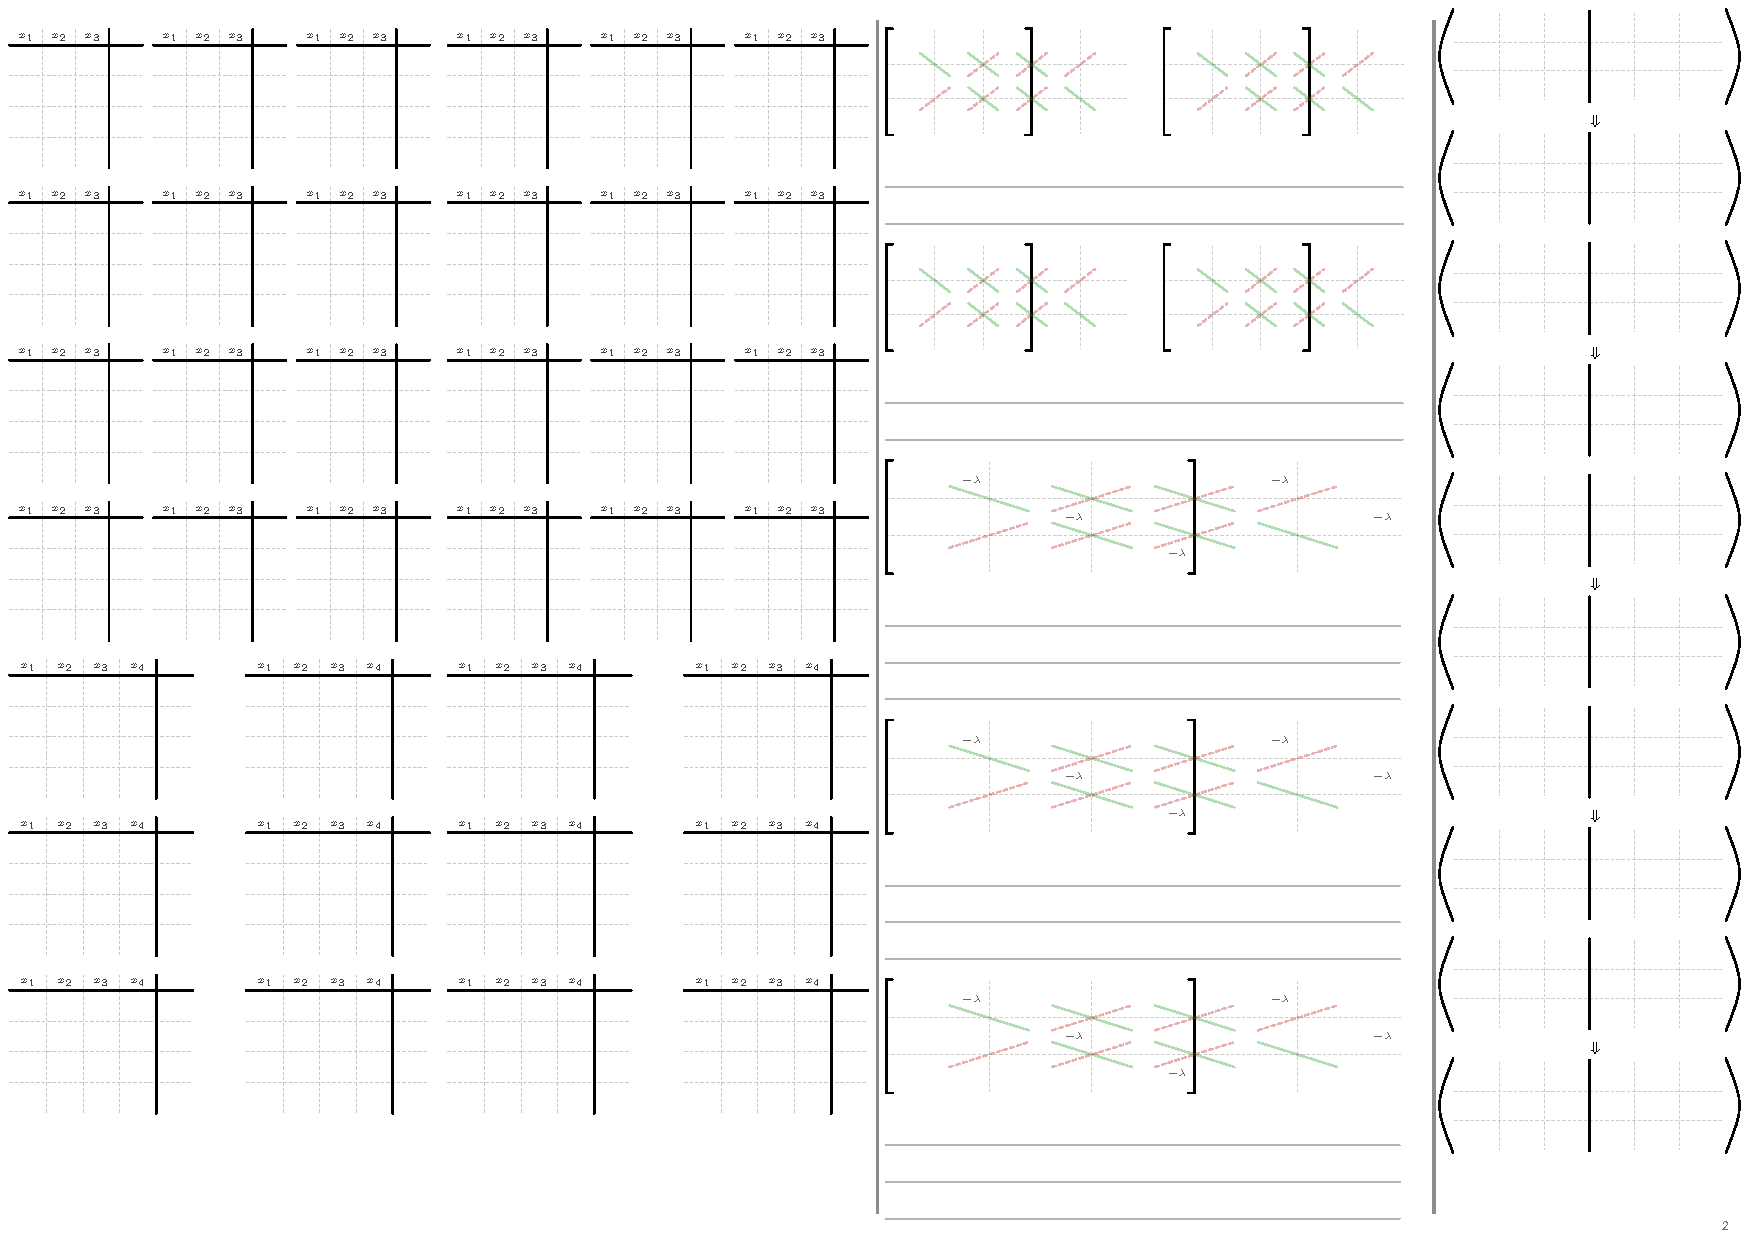
\includepdf[pages=-]{graphics/LinAlg_zsf_TimonRong.pdf}
\end{document}
